\documentclass[12pt]{article}
\usepackage{amsmath, amssymb, amsthm, enumerate, mdwlist, graphicx}
\usepackage[stable]{footmisc}
\title{MATH 235B -- Probability Theory\\Lecture Notes,  Winter 2011}
\author{Dan Romik\\Department of Mathematics, UC Davis}
%\date{Draft of \today}

\linespread{1.3}

\setlength\textwidth{6.5in}
\setlength\oddsidemargin{0in}
\setlength\topmargin{-0.3in}
\setlength\textheight{8.3in}


\newtheorem{thm}{Theorem}[section]
\newtheorem{conj}[thm]{Conjecture}
\newtheorem{prop}[thm]{Proposition}
\newtheorem{lem}[thm]{Lemma}
\newtheorem{lemma}[thm]{Lemma}
\newtheorem{claim}[thm]{Claim}
\newtheorem{cor}[thm]{Corollary}
\newtheorem{coro}[thm]{Corollary}
\newtheorem{defi}[thm]{Definition}
%\newtheorem{example}[thm]{Example}
\newtheorem{exercise}[thm]{Exercise}

\newcommand{\R}{\mathbb{R}}
\newcommand{\Z}{\mathbb{Z}}
\newcommand{\N}{\mathbb{N}}
\newcommand{\prob}{\mathbf{P}}
\newcommand{\expec}{\mathbf{E}}
\newcommand{\var}{\mathbf{V}}
\newcommand{\cov}{\textrm{Cov}}

\newcommand{\condexp}[2]{\expec\left(#1\,|\,#2\right)}
\newcommand{\condprob}[2]{\prob\left(#1\,|\,#2\right)}


\newcommand{\ind}{\textbf{1}}

\def\lecturesamepage#1{
  \addtocounter{section}{1}
  \setcounter{thm}{0}
  \section*{Chapter \arabic{section}: #1} 
  \setcounter{subsection}{0}
\addcontentsline{toc}{section}{Chapter \arabic{section}: #1}  
}
\def\lecture#1{
  \newpage
  \addtocounter{section}{1}
  \setcounter{thm}{0}
  \section*{Chapter \arabic{section}: #1} 
  \setcounter{subsection}{0}
\addcontentsline{toc}{section}{Chapter \arabic{section}: #1}  
}


 \newtheoremstyle{example}{\topsep}{\topsep}%
     {}%         Body font
     {}%         Indent amount (empty = no indent, \parindent = para indent)
     {\bfseries}% Thm head font
     {}%        Punctuation after thm head
     { }%     Space after thm head (\newline = linebreak)
     {\thmname{#1} \thmnumber{ #2.}\thmnote{ #3}}%         Thm head spec

\theoremstyle{example}
\newtheorem{example}[thm]{Example}

\begin{document}
\maketitle

%\vspace{100.0pt}
%\noindent
%\textbf{Note to the reader.} This is a first draft, so potentially contains various errors and inaccuracies. If you find any, please report them to me by email.

%\section*{Lecture 1: Introduction}
%\addtocounter{section}{1}
%\setcounter{subsection}{0}

\thispagestyle{empty}
%
\newpage
%
\tableofcontents


\newpage



\begin{center}
\LARGE
Part I --- Conditional Expectations and Martingales
\end{center}


\lecturesamepage{A motivating example for martingales}

A \textbf{martingale} is a mathematical model for a sequence of fair gambles which has found many applications in both theoretical and applied probability. (In particular, martingales play an important role in the mathematics of investing and other areas of mathematical finance --- so knowing about them can actually make you money!) One of the most important facts about martingales is that under fairly mild assumptions they converge (almost surely, or in $L_1$ or according to some other notion of convergence). This is made precise in a family of important results known as \emph{martingale convergence theorems}. Our goal in the next few chapters will be to develop the basic theory of martingales and its applications and prove some of the martingale convergence theorems.

We start our study of martingales with a motivating example: a famous experiment known as \textbf{P\'olya's urn experiment}. In this model, an urn originally contains $a$ white balls and $b$ black balls. The experimenter samples a uniformly random ball from the urn, examines its color, then puts the ball back and adds another ball of the same color; this is repeated to infinity. Let $X_n$ denote the number of white balls in the urn after the $n$th step. Clearly $X_0 = a$ and the distribution of $X_{n+1}$ can be expressed most naturally by conditioning on $X_n$, namely
\begin{equation}\label{eq:polya-conditional}
{X_{n+1}}_{\big| X_n = m} = 
\begin{cases} 
m+1 & \textrm{with probability }\frac{m}{n+a+b}, \\
m & \textrm{with probability }\frac{n+a+b-m}{n+a+b}. \\
\end{cases}
\end{equation}
It turns out that it is not too difficult to find an unconditional formula for the probability distribution of $X_n$. Let $I_n$ be the indicator random variable of the event that in the $n$th sampling step a white ball was drawn. First, an amusing observation is that the probability of observing a particular sequence of white/black samples in the first $n$ sampling steps is only dependent on the number of white and black balls. That is, for any sequence $(x_1,x_2,\ldots,x_n)\in \{0,1\}^n$
the probability $\prob(I_1 = x_1, \ldots, I_n = x_n)$ only depends on $k=\sum_{j=1}^n x_j$. To see this, note that if at a given stage $t$ of the experiment the urn contained $A$ white and $B$ black balls, the probability to draw ``white then black'' in the next two steps would be
$$ \frac{A}{t+a+b}\cdot \frac{B}{t+a+b+1}, $$
which is clearly equal to the probability of drawing ``black then white,'' given by
$$ \frac{B}{t+a+b}\cdot \frac{A}{t+a+b+1}. $$
Thus, permuting the 1's and 0's in the sequence $(x_1,\ldots,x_n)$ has no effect on the probability\footnote{A sequence of r.v.'s with this property is called \textbf{exchangeable}. There is an important result about such sequences (that we will not talk about here) called \textbf{De-Finetti's theorem}, which you might want to read about.}. It follows that for any such $(x_1,\ldots,x_n)$ with $\sum x_j=k$ we have
\begin{align}
\prob(I_j = x_j,\ j=1,\ldots,n) &= \prob(I_1=\ldots=I_k=1,\ I_{k+1}=\ldots=I_n=0)
\nonumber \\ &= \frac{a(a+1)\ldots(a+k-1)\cdot b(b+1)\ldots(b+n-k-1)}{(a+b)(a+b+1)\ldots(a+b+n)}.
\label{eq:polyaurn-formula}
\end{align}
Therefore the probability of having $p$ white balls after $n$ steps is
\begin{align*}
\prob(X_n = p) &= \binom{n}{p-a}
\prob(I_1=\ldots=I_{p-a}=1,\ I_{p-a+1}=\ldots=I_n=0)
\\ &=
\binom{n}{p-a}
\frac{a(a+1)\ldots(a+p-a-1)\cdot b(b+1)\ldots(b+n-p+a-1)}{(a+b)(a+b+1)\ldots(a+b+n)}
\end{align*}
for $a \le p \le n+a$. This formula is so explicit that it is easy to analyze the distribution of $X_n$ and show for example the convergence in distribution
\begin{equation} \label{eq:polya-beta-dist}
\frac{X_n}{n+a+b} \implies \textrm{Beta}(a,b).
\end{equation}
That is, the \emph{proportion} of white balls in the urn converges to a limiting beta distribution.

\begin{exercise} Prove \eqref{eq:polya-beta-dist}.
\end{exercise}

What about stronger notions of convergence such as convergence in probability or almost sure convergence? This seems like a harder question that requires understanding more about the \emph{joint} distribution of different $X_n$'s. It turns out that we also have almost sure convergence, that is, the limit
\begin{equation} \label{eq:polya-as-conv}
Y = \lim_{n\to\infty} \frac{X_n}{n+a+b}
\end{equation}
exists almost surely, and that the main relevant fact that guarantees that this convergence takes place is that the proportions $M_n = X_n/(n+a+b)$ form a martingale! To see what this means, note that
\eqref{eq:polya-conditional} can be rewritten in the form
$$ {M_{n+1}}_{\big| M_n = m/(n+a+b)} = 
\begin{cases} 
\frac{m+1}{n+a+b+1} & \textrm{with probability }\frac{m}{n+a+b}, \\
\frac{m}{n+a+b+1} & \textrm{with probability }\frac{n+a+b-m}{n+a+b}. \\
\end{cases}
$$
Thus, the value of $M_{n+1}$ can be either greater or smaller than the value of $M_n$, but the amounts by which it increases or decreases, weighted by the respective probabilities of each of these events, balance out, so that \emph{on average}, the value stays the same:
$$
\frac{m}{n+a+b} = \frac{m}{n+a+b}\cdot \frac{m+1}{n+a+b+1} +
\frac{n+a+b-m}{n+a+b} \cdot \frac{m}{n+a+b+1}
$$
The martingale property, which will immediately imply the a.s.\ convergence \eqref{eq:polya-as-conv} through the use of one of the martingale convergence theorems, is a generalization of this statement for arbitrary sequences $(M_n)_{n=1}^\infty$. It is written in the more abstract form:
$$ \condexp{M_{n+1}}{M_1,\ldots,M_n} = M_n. $$ 
In this equation, the quantity on the left represents a new kind of random variable that we still haven't discussed, a \emph{conditional expectation}. So, before developing the theory of martingales we need a good understanding of conditional expectations. This is the subject of the next chapter.


\lecture{Conditional expectations}

\subsection{Elementary conditional expectations}

Let $X$ and $Y$ be random variables defined on the same probability space $(\Omega, \mathcal{F}, \prob)$. We wish to generalize the expectation operator $\expec$ that takes a random variable $X$ and returns a number, to include the possibility of having additional information, encoded by the random variable $Y$. Thus, we want to define the \textbf{conditional expectation} $\condexp{X}{Y}$ (``the conditional expectation of $X$ given $Y$''). This is tricky to do for general random variables, so let's start with the simple case in which $X$ and $Y$ are both discrete random variables taking on finitely many values with positive probability. That is,
assume there are numbers $x_1,\ldots, x_m$ and $y_1,\ldots, y_n$ such that 
$$ \prob\left( X \in \{ x_1,\ldots, x_m\}, Y \in \{ y_1,\ldots, y_n \} \right) = 1. $$
In this case, if we know that $Y=y_j$ for some $1\le j\le n$, then the conditional distribution of $X$ becomes
$$ \prob(X = x_i\ |\ Y=y_j) = \frac{\prob(X=x_i, Y=y_j)}{\prob(Y=y_j)}, \qquad 1\le i\le m. $$
The expected value of this distribution is
$$ \condexp{X}{Y=y_j} = \sum_{i=1}^n \prob(X = x_i\ |\ Y=y_j) x_i. $$
For each $j$, this is a \emph{number}. It makes sense to define a \emph{random variable}, not a number, to be the random variable $Z=\condexp{X}{Y}$ that is equal to $\condexp{X=x_i}{Y=y_j}$ on the event $\{Y=y_j\}$:
$$ Z = \sum_{j=1}^n \condexp{X}{Y=y_j} \ind_{\{Y=y_j\}}. $$
Let us try to think of a more conceptual way to look at this definition. First of all, note that the actual values $y_1,\ldots, y_n$ that the random variable $Y$ takes are not so important. Rather, what is important is that $Y$ partitions the probability space $\Omega$ into disjoint subsets, such that knowing which of the subsets we end up in changes our view of the distribution of $X$. Therefore in the definition of $Z$ we could insert in place of $Y$ an object that encodes this slightly lesser information (i.e., not including the values of $Y$). It turns out that the correct object to use is the $\sigma$-algebra $\sigma(Y)$ generated by $Y$. For a general r.v., this is defined by
$$ \sigma(Y) = \big\{ \{Y \in B\}\ :\ B\in\mathcal{B}(\R) \big\}
= \{ Y^{-1}(B)\ :\ B\in\mathcal{B}(\R) \}
$$
and is a sub-$\sigma$-algebra of $\mathcal{F}$. For our discrete $Y$, it is the $\sigma$-algebra generated by the events $\{Y=y_j\}, \ j=1,\ldots,n$.
So, given a sub-$\sigma$-algebra $\mathcal{G} \subset \mathcal{F}$ generated by a family of disjoint subsets $A_1,\ldots,A_n \in \mathcal{F}$ that partitions $\Omega$, we can rewrite the definition of the conditional expectation as the random variable $Z = \condexp{X}{\mathcal{G}}$
(``the conditional expectation of $X$ given the $\sigma$-algebra $\mathcal{G}$'') given by
$$
Z = \sum_{j=1}^n \condexp{X}{A_j} \ind_{A_j}.
$$
Here, for each $1\le j\le n$ the quantity $\condexp{X}{A_j}$ is a number, the expected value of the conditional distribution of $X$ on the event $A_j$.

The next observation is that $Z$ satisfies two properties, which seem rather trivial and uninteresting in this context, but will turn out to be crucial to generalizing the definition of $\condexp{X}{Y}$ to arbitrary random variables:

\begin{enumerate}[(i)]
\item
$Z$ is measurable with respect to $\mathcal{G}$. That is, for each Borel set $B\in \mathcal{B}(\R)$, the event $\{Z\in B\} \in \mathcal{G}$. Equivalent ways of saying the same thing are that $\sigma(Z)\subset \mathcal{G}$, or that~$Z$ would remain a random variable even if we change the probability space to $(\Omega,\mathcal{G},\prob)$.

\item For any event $E \in \mathcal{G}$, we have $\expec(Z \ind_E) = \expec(X \ind_E)$.
\end{enumerate}

\begin{exercise} Prove the above two properties.
\end{exercise}


\subsection{General conditional expectations}

The above discussion brings us to the following important definition.

\begin{defi}
Let $X$ be a random variable on $(\Omega, \mathcal{F}, \prob)$ with $\expec|X|<\infty$, and let $\mathcal{G}$ be a sub-$\sigma$-algebra of~$\mathcal{F}$.
If a random variable $Z$ satisfies properties (i) and (ii) above, we say that $Z$ is the \textbf{conditional expectation of $X$ given $\mathcal{G}$}, and denote
$ Z = \condexp{X}{\mathcal{G}}$.
If~$Y$ is another random variable on $(\Omega, \mathcal{F}, \prob)$, then taking $\mathcal{G}=\sigma(Y)$ we may denote
$Z = \condexp{X}{Y} = \condexp{X}{\sigma(Y)}$, and refer to $Z$ as the \textbf{conditional expectation of $X$ given $Y$}.
\end{defi}

The use of the notation $ Z = \condexp{X}{\mathcal{G}}$ contains the implicit assumption that the conditional expectation is unique. This is true with the convention that random variables are defined only up to almost sure equivalence. That is, if $Z=Z'$ a.s.\ we consider $Z$ and $Z'$ to be the same random variable (in particular, any event involving $Z$ will have the same probability as the corresponding event involving $Z'$). In fact, we will prove the following result which also answers the key questions regarding existence and integrability.

\begin{thm} \label{thm-cond-ext}
The conditional expectation exists, is an integrable random variable, and is unique up to almost sure equivalence.
\end{thm}

\begin{proof}[Proof of integrability]
Let $A = \{ Z>0 \}$. By (i), $A, A^c \in \mathcal{G}$. Therefore by (ii), we have
\begin{align*}
\expec(Z \ind_A) &= \expec(X \ind_A) \le \expec\left( |X| \ind_A \right), \\
\expec(Z \ind_{A^c}) &= \expec(X \ind_{A^c}) \ge -\expec\left( |X| \ind_{A^c} \right),
\end{align*}
Subtracting the two equations gives
$$ \expec|Z| = \expec(Z\ind_A - Z\ind_{A^c}) \le \expec\left( |X| (\ind_A + \ind_{A^c}) \right) = \expec|X| < \infty.
$$
\end{proof}

\begin{proof}[Proof of uniqueness] Assume that $Z$ and $Z'$ both satisfy properties (i), (ii). It follows that
$$ \expec(Z \ind_A) = \expec(Z' \ind_A)\ \  \textrm{ for all }A \in \mathcal{G}. $$
For some $\epsilon>0$, take $A = \{ Z-Z' \ge \epsilon \}$ to get that
$$ 0 = \expec( (Z-Z')\ind_A ) \ge \epsilon \prob(A), $$
so $\prob(A) = 0$. Since $\epsilon$ was an arbitrary positive number, this implies that $Z\le Z'$ a.s. Reversing the roles of $Z$ and $Z'$ gives that also $Z'\le Z$ a.s., so $Z=Z'$ a.s., which proves the uniqueness claim.
\end{proof}

The most tricky part in defining conditional expectations is proving that they exist. The usual proof involves an application of an important result from measure theory, the Radon-Nikodym theorem, which we review in the next section.


\subsection{Absolute continuity and the Radon-Nikodym theorem}

We will formulate a version of the Radon-Nikodym theorem for probability spaces. The theorem involves the useful concept of absolute continuity of measures.

\begin{defi}
Let $P$ and $Q$ be two probability measures on a measurable space $(\Omega, \mathcal{F})$. We say that \textbf{$P$ is absolutely continuous with respect to $Q$}, and denote $P<<Q$, if for any $A\in\mathcal{F}$, if $Q(A)=0$ then $P(A)=0$.
\end{defi}

There is an interesting intuitive interpretation to the notion of absolute continuity. In many real-life situations involving probability we know the measurable space $(\Omega, \mathcal{F})$ but do not know which probability measure correctly describes the statistical distribution of the outcome of the experiment (for example, someone hands us a die to roll but we are not sure if it is a fair or loaded die). Say there are two possible measures, $P$ and $Q$, which we are considering. It makes sense to perform the experiment and try to guess which of $P$ and $Q$ is the correct one based on the result. If we are lucky, the result might fall into an event $A \in \mathcal{F}$ which has the property that $Q(A)=0$ but $P(A)>0$, in which case we will know that we can safely rule out $Q$. The relation $P<<Q$ means that this cannot happen; i.e., based on a single experiment, or even a finite number of repeated experiments, we can never rule out $Q$ as the correct measure, although we may become increasingly convinced that $P$ is the correct one as the statistical evidence mounts\footnote{The question of precisely how fast can one become convinced of the correct answer leads to the concept of \textbf{relative entropy}, which will be the subject of a future homework problem.}. If $P<<Q$ and $Q<<P$, meaning both measures are mutually absolutely continuous w.r.t.\ each other, we can also never rule out $P$ so we may never be entirely sure which measure correctly describes the experiment.

The following lemma sheds further light on the notion of absolute continuity. Its proof is a nice application of the first Borel-Cantelli lemma.

\begin{lem} \label{lem-abs-cont}
$P$ is absolutely continuous with respect to $Q$ if and only if for any $\epsilon>0$ there exists a $\delta>0$ such that if $Q(A)<\delta$ then $P(A)<\epsilon$.
\end{lem}

\begin{proof}
The ``if'' direction is immediate. To prove the ``only if,'' assume the negation of the condition ``for any $\epsilon>0$,  \ldots'' That is, there must exist an $\epsilon>0$ such that for any $\delta>0$ there is an event $A_\delta$ such that $Q(A_\delta)< \delta$ but $P(A_\delta)\ge\epsilon$. Now consider the event
$$ E= \{ A_{1/{2^n}}\textrm{ i.o.} \} =  \bigcap_{N=1}^\infty \bigcup_{n=N}^\infty A_{1/2^n}
$$
Since $\sum_{n=1}^\infty 2^{-n}<\infty$, by the Borel-Cantelli lemma we get that $Q(E)=0$. On the other hand,
$$ P(E) = \lim_{N\to\infty} P\left[\bigcup_{n=N}^\infty A_{1/2^n}\right] \ge \limsup_{N\to\infty} P(A_{1/2^n}) \ge \epsilon>0.
$$
This shows that $P$ is not absolutely continuous with respect to $Q$.
\end{proof}

If $Q$ is a probability measure on $(\Omega, \mathcal{F})$, one way to construct a probability measure $P$ for which $P<<Q$ is to let
\begin{equation}\label{eq:abs-cont-p-q}
P(E) = \expec_Q(Z \ind_E), \qquad (E\in \mathcal{F}).
\end{equation}
where $Z$ is some nonnegative random variable on the probability space $(\Omega,\mathcal{F},Q)$ satisfying $\expec(Z)=1$ (the notation $\expec_Q(\cdot)$ emphasizes that the expectation operator is the one associated with the probability measure $Q$). The Radon-Nikodym theorem says that this construction is the most general one possible.

\begin{thm}[The Radon-Nikodym theorem] $P<<Q$ if and only if there exists a random variable $Z$ on $(\Omega, \mathcal{F}, \prob)$, unique up to $Q$-a.s.-equivalence, such that $Z\ge 0$ a.s.\ and the relation $P(E) = \expec_Q (Z \ind_E)$ holds for any $E\in \mathcal{F}$. The random variable $Z$ is referred to as the \textbf{Radon-Nikodym derivative} of $P$ relative to $Q$ and denoted $$Z = \frac{dP}{dQ}. $$
\end{thm}

As mentioned above, the ``if'' part of the theorem is immediate, so it is really the ``only if'' part which is interesting. The Radon-Nikodym theorem has several classical proofs which may be read in measure theory and analysis textbooks. We will assume it without proof for now, and later sketch a probabilistic proof that uses martingale theory. (This is almost circular logic, since we will use conditional expectations to develop martingales and conditional expectations rely on the Radon-Nikodym theorem. However, with a bit of care one can make sure to use only the ``elementary'' version of conditional expectations and thus obtain a genuinely new proof that does not make use of circular reasoning --- this is one of the nice examples of probability theory ``giving back'' to the rest of mathematics.)

Note that the Radon-Nikodym derivative generalizes the ordinary derivative: if $Q$ is Lebesgue measure on the measure space $((0,1),\mathcal{B})$ and $P<<Q$, then the random variable~$Z$ in \eqref{eq:abs-cont-p-q} can be thought of as the density function of a random variable whose distribution measure is $P$, and can be computed as an actual derivative of the cumulative distribution function of this random variable, i.e.,
$$ Z(x) = \frac{d}{dx} P((0,x)) \quad\textrm{a.s.} $$
Another reason why it makes sense to think of $Z$ as a kind of ``derivative'' is that if one uses the Lebesgue integral notation $\int_E Z dQ$ instead of our more probabilistic notation $\expec_Q(Z\ind_E)$, the relation \eqref{eq:abs-cont-p-q} can be rewritten as an intuitive ``change of measures'' formula
\begin{equation} \label{eq:abs-cont-change-var} 
\int_E dP = \int_E \frac{dP}{dQ} dQ.
\end{equation}

\begin{exercise}
Prove that if $P<<Q$ are two probability measures on a measurable space $(\Omega, \mathcal{F})$ then \eqref{eq:abs-cont-change-var} generalizes to the identity
$$
\int_E X dP = \int_E X \frac{dP}{dQ} dQ
$$
which holds for any random variable $X$ for which $\expec_P|X|<\infty$.
\end{exercise}


\begin{proof}[Proof of existence in Theorem~\ref{thm-cond-ext}] We are now in a position to prove the existence of conditional expectations. Assume first that $X\ge 0$. Define the measure $Q$ on the measurable space $(\Omega, \mathcal{G})$ by
$$ Q(E) = \expec_\prob(X \ind_E), \qquad E\in\mathcal{G}. $$
Note that $Q$ is not a \emph{probability} measure; rather, it is a \emph{finite} measure, which is like a probability measure but takes values in $[0,\infty)$ and is not required to satisfy $Q(\Omega)=1$. However, the Radon-Nikodym theorem remains true for such measures (even more generally for so-called \emph{$\sigma$-finite} measures), as can easily be seen by replacing $Q(\cdot)$ by its scalar multiple $Q(\Omega)^{-1} Q(\cdot)$, which is a probability measure.
Now, the original probability measure $\prob$ on $(\Omega, \mathcal{F})$ can also be thought of as a measure on the measurable space $(\Omega, \mathcal{G})$. Furthermore, it is easy to see that $Q << \prob$.
% (This follows from the monotone convergence theorem --- check!) 
Thus, we are exactly in the situation described in the Radon-Nikodym theorem, and we conclude that there is a random variable $Z=dQ/dP$, measurable with respect to the $\sigma$-algebra $\mathcal{G}$, such that for any $E\in\mathcal{G}$ we have
$$ \expec_\prob(Z \ind_E) = Q(E) = \expec_\prob(X \ind_E). $$
Thus, $Z$ satisfies the two properties (i)--(ii) in the definition of the conditional expectation, so the conditional expectation $Z=\condexp{X}{\mathcal{G}}$ exists.

Finally, for a general random variable $X$ with $\expec|X|<\infty$, write $X=X_+-X_-$ where $X_+, X_-\ge 0$ are the non-negative and non-positive parts of $X$, respectively. It is immediate to check that the random variable $Z = \condexp{X_+}{\mathcal{G}}
- \condexp{X_-}{\mathcal{G}}$ satisfies the properties (i)--(ii) required of the conditional expectation $\condexp{X}{\mathcal{G}}$, so again we have shown that the conditional expectation exists.
\end{proof}


\subsection{Properties and examples of conditional expectations}

\begin{enumerate}
\item If $X$ is measurable with respect to $\mathcal{G}$ (i.e., $\sigma(X) \subset \mathcal{G}$) then
$\condexp{X}{\mathcal{G}} = X$. The intuition is that if the information given to us (encoded by the $\sigma$-algebra $\mathcal{G}$) is enough to tell the value of $X$ (see the exercise below), then our best guess for the average value of $X$ is $X$ itself.

\begin{exercise}
Let $X$ and $Y$ be random variables defined on the same probability space $(\Omega, \mathcal{F}, \prob)$. Show that $\sigma(X) \subset \sigma(Y)$ (in this case we say that \textbf{$X$ is measurable with respect to $Y$}) if and only if there exists a Borel-measurable function $h:\R\to\R$ such that $X=h(Y)$~a.s.
\end{exercise}


\item In particular, if $\mathcal{G}=\mathcal{F}$ is the original $\sigma$-algebra of the probability space $(\Omega, \mathcal{F}, \prob)$, then $\condexp{X}{\mathcal{G}} = X$.
\item At the opposite extreme, if $\mathcal{G}= \{ \emptyset, \Omega \}$, then $\condexp{X}{\mathcal{G}} = \expec(X)$, the usual expectation of $X$. Intuitively, the minimal $\sigma$-algebra $\{\emptyset, \Omega\}$ represents zero information.

\item More generally, if $X$ is independent of $\mathcal{G}$ then $\condexp{X}{\mathcal{G}}=\expec(X)$, since $\expec(X)$ is a $\mathcal{G}$-measurable random variable and for any $E\in\mathcal{G}$, since $X$ is independent of $\ind_E$,
$$\expec(X\ind_E) = \expec(X)\expec(\ind_E) = \expec(\expec(X)\ind_E). $$

\item Conditional expectation is a linear operator: $\condexp{aX+bY}{\mathcal{G}} = a \condexp{X}{\mathcal{G}} + b \condexp{Y}{\mathcal{G}}.$

\begin{proof}
The random variable $Z=a \condexp{X}{\mathcal{G}} + b \condexp{Y}{\mathcal{G}}$ is $\mathcal{G}$-measurable and for any $E\in\mathcal{G}$ we have
\begin{align*} \expec(Z\ind_E) &= a\expec(\condexp{X}{\mathcal{G}}\ind_E)+b\expec(\condexp{Y}{\mathcal{G}}\ind_E) = 
a \expec(X\ind_E)+b\expec(Y\ind_E) \\&=\expec((aX+bY)\ind_E),
\end{align*}
so $Z$ satisfies the requirements that qualify it to be the conditional expectation of $aX+bY$.
\end{proof}


\item Monotonicity: If $X\le Y$ then $\condexp{X}{\mathcal{G}}\le\condexp{Y}{\mathcal{G}}$ a.s.

\begin{proof}
For any $E\in\mathcal{G}$, we have that
$$ \expec(\condexp{X}{\mathcal{G}}\ind_E) = \expec(X\ind_E) \le
\expec(Y\ind_E) \le \expec(\condexp{Y}{\mathcal{G}}\ind_E). $$
Taking $E=\{\condexp{X}{\mathcal{G}}-\condexp{Y}{\mathcal{G}}\ge \epsilon\}$ for some arbitrary $\epsilon>0$, we get that $E$ must have probability $0$. Since this is true for any $\epsilon>0$, the result follows.
\end{proof}


\item Conditional form of the monotone convergence theorem: If $X_n\ge 0$ and $X_n \uparrow X$ a.s.\ as $n\to\infty$, where $\expec(X)<\infty$, then $\condexp{X_n}{\mathcal{G}}\nearrow \condexp{X}{\mathcal{G}}$ a.s.\ as $n\to\infty$.

\begin{proof}
By the monotonicity proved above, the conditional expectations $\condexp{X_n}{\mathcal{G}}$ are increasing to an a.s.\ limiting r.v.\ $Z$, which is $\mathcal{G}$-measurable. Note that $\condexp{X_n}{\mathcal{G}}\le \condexp{X}{\mathcal{G}}$, which is an integrable upper bound, so we can apply the dominated convergence theorem and deduce that for every $E\in \mathcal{G}$,
$$ \expec(Z\ind_E) = \expec(\lim_{n\to\infty} \condexp{X_n}{\mathcal{G}}\ind_E)
= \lim_{n\to\infty} \expec(\condexp{X_n}{\mathcal{G}}\ind_E) = \lim_{n\to\infty} \expec(X_n\ind_E)
= \expec(X\ind_E). 
$$
Thus $Z$, qualifies as the conditional expectation of $X$ given $\mathcal{G}$.
\end{proof}


\item Conditional form of Jensen's inequality: If $\varphi:\R\to\R$ is a convex function and $\expec|X|, \expec|\varphi(X)|<\infty$ then
$ \varphi(\condexp{X}{\mathcal{G}}) \le \condexp{\varphi(X)}{\mathcal{G}}. $

\begin{proof} The proof is similar to the non-conditional case, with a small twist: we observe that $\varphi(x)$ is a supremum of a countable number of linear functions, namely
$$ \varphi(x) = \sup \{ ax+b\,:\,a,b\in \mathbb{Q}, ax+b\le \varphi(x)\textrm{ for all }x\}, $$
then continue as in the original proof. The restriction to a countable number of linear functions is necessary since all statements pertaining to conditional expectations are almost sure statements, which means that there is an exceptional $0$-probability set being discarded, and we can only allow a countable number of these.
\end{proof}

\item For $p\ge 1$, $\expec\left( \left|\condexp{X}{\mathcal{G}}\right|^p \right) \le \expec|X|^p$ (i.e., the conditional expectation operator is a contraction in~$L_p(\Omega,\mathcal{G},\prob)$.)

\begin{proof}
By Jensen's inequality, $|\condexp{X}{\mathcal{G}}|^p \le \condexp{|X|^p}{\mathcal{G}}$. Now take expectations and use the fact that:
\end{proof}

\item $\expec(\condexp{X}{\mathcal{G}}) = \expec(X)$. This is a special case of:

\item If $\mathcal{G}_1\subseteq \mathcal{G}_2 \subseteq \mathcal{F}$ are sub-$\sigma$-algebras then we have
\begin{align*}
\condexp{\condexp{X}{\mathcal{G}_2}}{\mathcal{G}_1} &= \condexp{X}{\mathcal{G}_1}, \\
\condexp{\condexp{X}{\mathcal{G}_1}}{\mathcal{G}_2} &= \condexp{X}{\mathcal{G}_1},
\qquad  \textrm{(no, there is no typo here\ldots)}
\end{align*}


\begin{exercise} Prove this. \end{exercise}

\item If $X$ is $\mathcal{G}$-measurable, then for any random variable $Y$, if $\expec|Y|, \expec|XY|<\infty$ then
$$ \condexp{XY}{\mathcal{G}} = X \condexp{Y}{\mathcal{G}}.$$
The idea here is that if $X$ is measurable with respect to $\mathcal{G}$ then it appears like a constant from the point of view of conditional expectations given the information contained in $\mathcal{G}$ and can therefore be ``pulled outside'' of the expectation.

\begin{proof}
The random variable $Z=X\condexp{Y}{\mathcal{G}}$ is $\mathcal{G}$-measurable, so we need to check that for any $E\in \mathcal{G}$, 
\begin{equation}\label{eq:condexp-x-times-y}
\expec(Z\ind_E) = \expec(XY \ind_E).
\end{equation}
First, if $X=\ind_B$ for some $B\in\mathcal{G}$ then
$$ \expec(Z \ind_E) = \expec(\condexp{Y}{\mathcal{G}}\ind_{B\cap E}) = \expec(Y\ind_{B\cap E})
= \expec(XY \ind_E)
$$
so the claim is true. By linearity it follows that if $X$ is a ``simple'' random variable (a linear combination of finitely many indicator variables, i.e., a random variable taking finitely many values) then \eqref{eq:condexp-x-times-y} still holds. Now, assume that $X,Y\ge 0$, then we can take a sequence $(X_n)_{n=1}^\infty$ of simple random variables that are $\mathcal{G}$-measurable and such that $X_n\uparrow X$. By the monotone converegence theorem, it follows that \eqref{eq:condexp-x-times-y} holds also in this case. Finally, for general $X,Y$ one proves \eqref{eq:condexp-x-times-y} by splitting $X$ and $Y$ into their positive and negative parts.
\end{proof}


\end{enumerate}

\subsection{Conditional expectation as the least mean square error estimator}

In this section we show that the conditional expectation is actually the solution to a very natural estimation problem. Let $X$ be a random variable with finite variance. Assume that we wish to give the best possible estimate for the value of $X$, but only have access to the information encoded by the $\sigma$-algebra $\mathcal{G}$ (i.e., for each event $E\in\mathcal{G}$ we know if $E$ occurred or did not occur). Our estimate will therefore be some random variable $Y$ which is $\mathcal{G}$-measurable. A natural measure for the quality of the estimate is the \textbf{mean square error}
$$ \operatorname{MSE}_X(Y) = \expec(X-Y)^2. $$
The problem of finding the $Y$ that minimizes this error is very natural and of great practical importance. Its solution is given in the following theorem.

\begin{thm} If $\expec(X^2)<\infty$, then $\condexp{X}{\mathcal{G}}$ is the unique (up to a.s.\ equivalence) random variable $Y$ that minimizes the mean square error $\operatorname{MSE}_X(Y)$ among all $\mathcal{G}$-measurable random variables.
\end{thm}

\begin{proof} Denote $Z=\condexp{X}{\mathcal{G}}$. If $Y$ is a $\mathcal{G}$-measurable random variable with $\expec Y^2<\infty$ (if $Y$ does not have finite variance then clearly the MSE will be infinite), then
\begin{align*}
\expec(X-Y)^2 &= \expec[((X-Z)-(Y-Z))^2]
\\ &= \expec(X-Z)^2 + \expec(Y-Z)^2
+ 2 \expec[(X-Z)(Y-Z)]
\end{align*}
Denote $W=Y-Z$. This is a $\mathcal{G}$-measurable random variable, so by one of the properties proved in the previous section,
$$ \expec(WX) = \expec(\condexp{WX}{\mathcal{G}})
= \expec(W \condexp{X}{\mathcal{G}}) = \expec(WZ)
$$
(note that $\expec|WX|\le (\expec W^2 \expec X^2)^{1/2}<\infty$ by the Cauchy-Schwartz inequality) and therefore $\expec[(X-Z)(Y-Z)] = \expec[(X-Z)W]=0$. We get that
$$
\expec(X-Y)^2 = \expec(X-Z)^2 + \expec(Y-Z)^2, $$
which is clearly minimized when (and only when) $Y=Z$ a.s.
\end{proof}

The above result has an interesting geometric interpretation. The expression $\expec(X-Y)^2$ is the square of the $L_2$-distance between $X$ and $Y$ in the Hilbert space $L_2(\Omega, \mathcal{F},\prob)$. The theorem says that the conditional expectation operator $\condexp{\cdot}{\mathcal{G}}$ takes a random variable $X$ and returns the closest point to $X$ in the linear subspace $L_2(\Omega, \mathcal{G},\prob)\subset L_2(\Omega, \mathcal{F},\prob)$ consisting of square-integrable $\mathcal{G}$-measurable random variables. By elementary properties of Hilbert spaces, this is equivalent to the statement that $\condexp{\cdot}{\mathcal{G}}$ is the orthogonal projection operator onto the subspace $L_2(\Omega, \mathcal{G},\prob)$. 

One way in which this geometric interpretation is useful is that it suggests an alternative approach to defining conditional expectations that does not rely on the Radon-Nikodym Theorem: first construct the conditional expectation operator $\condexp{\cdot}{\mathcal{G}}$ for square-integrable random variables by defining it as an orthogonal projection operator; then extend the definition to the space $L_1(\Omega,\mathcal{F},\prob)$ of integrable random variables by approximating such variables by square-integrable ones. The book \textit{Probability With Martingales} by David Williams is one textbook where such an approach is developed. 


\lecture{Martingales}

\subsection{Definition and examples}

We are ready to start studying the processes known as martingales, which generalize the ``balancing'' property exhibited by the fraction of white balls in the Poly\'a urn experiment.

Let $(\Omega, \mathcal{F}, \prob)$ be a probability space, equipped with an increasing family
$$ \mathcal{G}_1 \subset \mathcal{G}_2 \subset \mathcal{G}_3 \subset \ldots $$
of sub-$\sigma$-algebras of $\mathcal{F}$. We refer to such a family $(\mathcal{G}_n)_{n=1}^\infty$ as a \textbf{filtration}. The $n$th $\sigma$-algebra $\mathcal{G}_n$ represents the state of knowledge (of an experimenter) about the probabilistic world $(\Omega, \mathcal{F}, \prob)$ at time $n$. A sequence of random variables $(X_n)_{n=1}^\infty$ is said to be \textbf{adapted to the filtration $(\mathcal{G}_n)_{n=1}^\infty$} if $X_n$ is $\mathcal{G}_n$-measurable for any $n$; that is, if the $n$th value in the sequence is known at time $n$.

\begin{defi}
Given a filtration $(\mathcal{G}_n)_{n=1}^\infty$, a sequence $(X_n)_{n=1}^\infty$ of random variables is called a \textbf{martingale} with respect to the filtration if it satisfies:
\begin{enumerate}[M1.]
\item $\expec|X_n|<\infty$ for all $n\ge1$.
\item The sequence $(X_n)_{n=1}^\infty$ is adapted to the filtration $(\mathcal{G}_n)_{n=1}^\infty$.
\item $\condexp{X_{n+1}}{\mathcal{G}_n} = X_n$ for all $n\ge 1$.
\end{enumerate}
If instead of property M3.\ the sequence satisfies the condition $\condexp{X_{n+1}}{\mathcal{G}_n} \ge X_n$, it is called a \textbf{submartingale}. If it satisfies
$\condexp{X_{n+1}}{\mathcal{G}_n} \le X_n$, it is called a \textbf{supermartingale}

\end{defi}

\begin{example} (Simple random walk).
Let $X_1, X_2, \ldots, $ be a sequence of i.i.d. random variables with $\prob(X_n=1)=\tfrac12$, $\prob(X_n=-1)=\tfrac12$. Denote $S_n = \sum_{k=1}^n X_n$. Define the filtration $(\mathcal{G}_n)_n$ by $\mathcal{G}_n = \sigma(X_1,\ldots,X_n)$ (the $\sigma$-algebra generated by the first $n$ random signs). Then the sequence $(S_n)_{n=1}^\infty$ (known as ``simple symmetric random walk on $\Z$'') is a martingale with respect to $(\mathcal{G}_n)_n$, since
$$ \condexp{S_n}{\mathcal{G}_{n-1}} = \condexp{S_{n-1}+X_n}{\mathcal{G}_{n-1}}
= S_{n-1} + \condexp{X_n}{\mathcal{G}_{n-1}} = S_{n-1} + \expec(X_n) = S_{n-1}.
$$
\end{example}

\begin{example} (Random walk with balanced steps).
More generally, the cumulative sums $S_n=\sum_{k=1}^n S_n$ of an i.i.d.\ sequence $X_1,X_2,\ldots$ where $X_n\sim F$ (the random walk with i.i.d. steps distributed according to $F$) is a martingale with respect to the filtration $\mathcal{G}_n=\sigma(X_1,\ldots,X_n)$ if $\expec(X_1)=0$. Even more generally, the r.v.'s $X_1,X_2,\ldots$ can be assumed to be independent but not identically distributed; if for any $n$ we have that $\expec|X_n|<\infty$ and $\expec X_n = 0$, then (by the same computation as above) $S_n$ is a martingale.
\end{example}

\begin{example} (Revealing information). Let $X$ be a random variable and let $(\mathcal{G}_n)_{n=1}^\infty$ be a filtration. The sequence $(X_n)_{n=1}^\infty$ defined by
$ X_n = \condexp{X}{\mathcal{G}_n} $
is a martingale. Intuitively, it is the sequence of better and better estimates for the value of $X$ that we can make as more and more information (represented by the filtration) is revealed.
\end{example}

It is not difficult to check that if $(X_n)_{n=1}^\infty$ is a martingale with respect to a filtration $(\mathcal{G}_n)_{n=1}^\infty$ then $(X_n)_{n=1}^\infty$ is also a martingale with respect to its ``natural'' filtration $\mathcal{H}_n=\sigma(X_1,\ldots,X_n) \subset \mathcal{G}_n$. This illustrates the fact that the filtration $(\mathcal{G}_n)$ usually doesn't play a very major role, but is simply a convenient way to represent the information that is used to compute the sequence.

\begin{example} (Discrete harmonic functions on a graph). Let $G=(V,E)$ be a graph (assume $V$ is finite or countable). A function $h:V\to\R$ is called \textbf{harmonic} if it satisfies the ``mean value'' property
$$ h(x) = \frac{1}{\operatorname{deg}(x)}\sum_{y \sim x} h(y) \qquad (x\in V), $$
where the notation $y\sim x$ means that $x,y$ are neighbors and $\operatorname{deg}(x)$ is the number of neighbors (the degree of $x$).
Let $X_0,X_1,X_2,\ldots$ be a \textbf{simple random walk on $G$}; that is, each $X_n$ is a $V$-valued random variable, and the distribution of $X_{n+1}$ is defined conditionally on $X_n$ by
$$ \prob(X_{n+1} = y\,|\,X_n=x) = \begin{cases} \frac{1}{\operatorname{deg}(x)} & y\sim x, \\ 0 & y\nsim x.
\end{cases}
$$
The starting point $X_0$ of the walk can be a deterministic vertex $x$ or a distribution on $V$. Let $\mathcal{G}_n=\sigma(X_0,\ldots,X_n)$. Define a sequence of real-valued random variables by $M_n = h(X_n)$. 
As an exercise, we leave to the reader to check that 
%$$
%\condexp{M_{n+1}}{\mathcal{G}_n} =  % *** finish this ***
%$$
%so 
$(M_n)_{n=0}^\infty$ is a martingale with respect to the filtration $(\mathcal{G}_n)_{n=0}^\infty$
\end{example}

\begin{example} (``Double or nothing''). Let $X_1,X_2,\ldots $ be an i.i.d.\ sequence of random variables satisfying
$ \prob(X_n = 0) = \tfrac12, \prob(X_n = 2) = \tfrac12$. Let $\mathcal{G}_n=\sigma(X_1,\ldots,X_n)$. Define $M_n = \prod_{k=1}^n X_n$. Then
$$ \condexp{M_{n+1}}{\mathcal{G}_{n}} = \condexp{M_{n} X_{n+1}}{\mathcal{G}_n} = M_{n} \condexp{X_{n+1}}{\mathcal{G}_n} = M_{n} \expec{X_{n+1}} = M_n, $$
so $(M_n)_{n=1}^\infty$ is a martingale with respect to the filtration $(\mathcal{G}_n)_{n=1}^\infty$. The meaning of the name ``double or nothing'' should be obvious.
\end{example}

\begin{example} (Multiplicative random walk). The previous example is a special case of the following situation: let $X_1, X_2, \ldots $ be an i.i.d. sequence of nonnegative random variables with $\expec(X_1)=1$. Then by the same computation as above, $M_n = \prod_{k=1}^n X_k$ is a martingale with respect to the filtration $\mathcal{G}_n = \sigma(X_1,\ldots,X_n)$.
\end{example}

\begin{example} (Alexander Calder mobile sculptures). The mobile sculptures pioneered by the American sculptor Alexander Calder are a mechanical manifestation of a martingale (Figure~\ref{fig-calder-mobiles}).
\begin{figure}[h!]
\begin{center}
\scalebox{0.7}{
\includegraphics{figures/caldermobile1.jpeg}}
\scalebox{0.7}{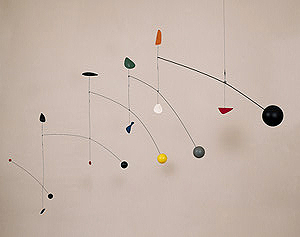
\includegraphics{figures/caldermobile2.jpg}}
\caption{Some mobiles by Alexander Calder}
\label{fig-calder-mobiles}
\end{center}
\end{figure}

The idea is that the $n$th random variable corresponds to the horizontal displacement of a ``node'' in the mobile as one descends the tree of nodes starting from the upper support point of the mobile. The fact that the tree is in static equilibrium corresponds to the statement that the center of mass of the subtree supported below each node is at the same horizontal displacement as the node itself, which can be thought of as a version of the martingale equation $\condexp{X_{n+1}}{\mathcal{G}_n} = X_n$.
\end{example}

\begin{example} (Whippletrees). Another real-life example of the martingale idea is in the mechanical device known as a \textbf{whippletree}, used to divide force evenly between several draught animals towing a load (Figure~\ref{fig-whippletree}).

\begin{figure}[h!]
\begin{center}
\scalebox{0.4}{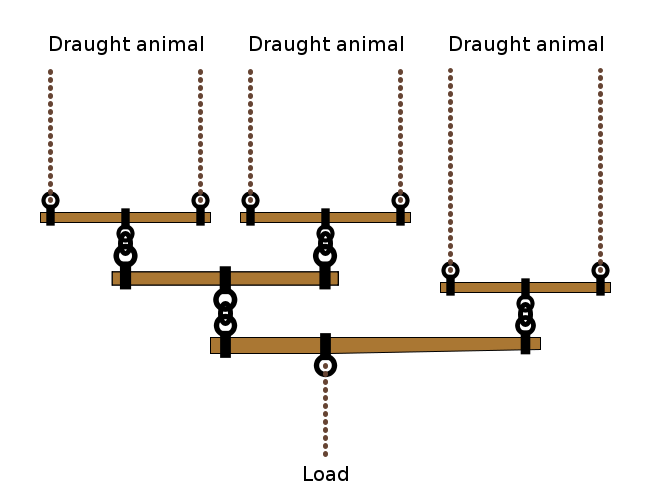
\includegraphics{figures/whippletree.png}}
\caption{An illustration of a whippletree (source: Wikipedia)}
\label{fig-whippletree}
\end{center}
\end{figure}
\end{example}

\begin{thm}
\begin{enumerate}
\item If $(X_n)_{n=1}^\infty$ is a martingale w.r.t.\ a filtration $(\mathcal{G}_n)_{n=1}^\infty$, then for $m< n$, $\condexp{X_n}{\mathcal{G}_m} = X_m$.
\item If $(X_n)_{n=1}^\infty$ is a supermartingale w.r.t.\ $(\mathcal{G}_n)_{n=1}^\infty$, then for $m< n$, $\condexp{X_n}{\mathcal{G}_m} \le X_m$.
\item If $(X_n)_{n=1}^\infty$ is a submartingale w.r.t.\ $(\mathcal{G}_n)_{n=1}^\infty$, then for $m< n$, $\condexp{X_n}{\mathcal{G}_m} \ge X_m$.
\end{enumerate}
\end{thm}

\begin{proof}
It is enough to prove claim 2., since 3.\ follows by applying 2. to $-X_n$, and 1.~follows by combining 2.~and~3.
Assume $X_n$ is a supermartingale, then $X_m\ge \condexp{X_{m+1}}{\mathcal{G}_m}$ by the definition, and by induction on $k$, $X_m\ge \condexp{X_{m+k}}{\mathcal{G}_m}$, since if we showed this for $k-1$ then we have that
\begin{align*}
X_m &\ge \condexp{X_{m+1}}{\mathcal{G}_m}
\ge \condexp{\condexp{X_{m+1+(k-1)}}{\mathcal{G}_{m+1}}}{\mathcal{G}_m}
= \condexp{X_{m+k}}{\mathcal{G}_m}.
\end{align*}
\end{proof}

\begin{thm} 
\begin{enumerate}
\item If $(X_n)_n$ is a martingale w.r.t.\ $(\mathcal{G}_n)_n$ and $\varphi:\R\to\R$ is a convex function such that $\expec|\varphi(X_n)|<\infty$ for all $n$, then $(\varphi(X_n))_n$ is a submartingale.
\item If $(X_n)_n$ is a submartingale w.r.t.\ $(\mathcal{G}_n)_n$ and $\varphi:\R\to\R$ is a weakly increasing convex function such that $\expec|\varphi(X_n)|<\infty$ for all $n$, then $(\varphi(X_n))_n$ is a submartingale.
\end{enumerate}
\end{thm}

\begin{proof}
By Jensen's inequality,
$ \condexp{\varphi(X_{n+1})}{\mathcal{G}_n} \ge \varphi\left(\condexp{X_{n+1}}{\mathcal{G}_n}\right)$, and this is $= \varphi(X_n)$ in the case of the first claim, or $\ge \varphi(X_n)$ in the case of the second.
\end{proof}

\begin{cor} Let $p\ge 1$. If $(X_n)_n$ is a martingale w.r.t.\ $(\mathcal{G}_n)_n$ and $\expec|X_n|^p<\infty$ for all $n$, then $|X_n|^p$ is a submartingale w.r.t.\ $(\mathcal{G}_n)_n$.
\end{cor}

\begin{cor} \label{cor-positive-part}
\begin{enumerate}
\item If $(X_n)_{n=1}^\infty$ is a submartingale then $\big((X_n-a)_+\big)_{n=1}^\infty$ is a submartingale (where for a real number $x$, $x_+ = \max(x,0)$ is the positive part of $x$).
\item If $(X_n)_{n=1}^\infty$ is a supermartingale then for any $a\in\R$, $(X_n\wedge a)_{n=1}^\infty$ is a supermartingale.
\end{enumerate}

\end{cor}


\subsection{The martingale transform and investment strategies}

Let $(\mathcal{G}_n)_{n=0}^\infty$ be a filtration. Assume that we are given a sequence $(X_n)_{n=0}^\infty$ that is adapted to the filtration. Each increment $X_n-X_{n-1}$ can be thought of as representing an investment opportunity at time $n$. For example, $X_n$ can represent the price of a stock or other financial asset (which in the lingo of finance is referred to, somewhat  ironically, as a ``security'') on day $n$, so that $X_n-X_{n-1}$ will be the gain or loss of an investor holding one unit of the asset during day $n$. The \textbf{martingale transform} $H\bullet X$ is a new sequence of random variables representing the accumulated profits of an investor employing a predefined investment strategy, represented by a sequence $(H_n)_{n=1}^\infty$.\footnote{The name ``martingale transform'' is a poor choice, as it seems to imply that $H\bullet X$ is defined only when $(X_n)_n$ is a martingale. This is not the case, although it's true that the most interesting cases are when $(X_n)_n$ is a submartingale or supermartingale or both.}

To make this more precise, we say that a sequence $(H_n)_{n=1}^\infty$ is \textbf{predictable} with respect to the filtration $(\mathcal{G}_n)_{n=0}^\infty$ if for any $n\ge 1$, $H_n$ is $\mathcal{G}_{n-1}$-measurable. Think of $H_n$ as representing the number of investment units the investor holds during the $n$th trading day. An investment strategy must have this property, since (unless the investor is equipped with a crystal ball) the decision of how much to invest at time $n$ must depend only on information available at time $n-1$. Given a $(\mathcal{G}_n)_n$-adapted sequence $(X_n)_{n=0}^\infty$ and a predictable sequence $(H_n)_{n=1}^\infty$, we define the sequence $H\bullet X$ by
$$ (H\bullet X)_n = \sum_{m=1}^n H_m(X_m-X_{m-1}). $$

\begin{thm} \label{thm-marting-transform}
\begin{enumerate}
\item If $(X_n)_{n=0}^\infty$ is a supermartingale and $(H_n)_{n=1}^\infty$ is predictable, and for any~$n$, $H_n$ is bounded and nonnegative, then $H\bullet X$ is a supermartingale.
\item If $(X_n)_{n=0}^\infty$ is a submartingale and $(H_n)_{n=1}^\infty$ is predictable, and for any~$n$, $H_n$ is bounded and nonnegative, then $H\bullet X$ is a submartingale.
\item If $(X_n)_{n=0}^\infty$ is a martingale and $(H_n)_{n=1}^\infty$ is predictable, and for any~$n$, $H_n$ is bounded, then $H\bullet X$ is a martingale.
\end{enumerate}
\end{thm}

\begin{proof} We prove the first claim (the other ones are similar). It is obvious that $(H\bullet X)_n$ is adapted to $(\mathcal{G}_n)_n$, and furthermore, by the assumptions that $H_n$ is bounded and nonnegative, and the usual properties of conditional expectation, we get that
\begin{align*}
\condexp{(H\bullet X)_{n+1}}{\mathcal{G}_n} &= 
\condexp{(H\bullet X)_{n}}{\mathcal{G}_n} + 
\condexp{H_{n+1}(X_{n+1}-X_n)}{\mathcal{G}_n}
\\ &= (H\bullet X)_n +
H_{n+1} \condexp{X_{n+1}-X_n}{\mathcal{G}_n} \le (H\bullet X)_n.
\end{align*}
\end{proof}

A random variable $N$ taking values in $\{1,2,\ldots\}\cup \{\infty\}$ is said to be a \textbf{stopping time} with respect to the filtration $(\mathcal{G}_n)_{n=0}^\infty$ if for any $n\ge0$, the event $\{ N=n \}$ is in $\mathcal{G}_n$. That means that the decision to stop at time~$n$ depends only on information available at that time. Given a stopping time $N$, one possible investment strategy (a version of the classic ``buy and hold'') is to buy one investment unit at time $0$ and hold it until time $N$. In other words, we may define a sequence $(H_n)_n$ by
$$ H_n = \ind_{\{n\le N\}}, \qquad n\ge 1. $$
Note that $\{ n\le N\} = \{N\le n-1\}^\textrm{c} \in \mathcal{G}_{n-1}$, so $(H_n)_n$ is a predictable sequence, and we have
$$ (H\bullet X)_n = X_{N\wedge n} - X_0. $$

\begin{thm} \label{thm-stopping-mart}
If $N$ is a stopping time and $(X_n)_{n=0}^\infty$ is a supermartingale (respectively, submartingale, martingale), then $(X_{n\wedge N})_{n=0}^\infty$ is a supermartingale (respectively, submartingale, martingale).
\end{thm}

\begin{proof}
By Theorem~\ref{thm-marting-transform}, $X_{N\wedge n} - X_0$ is a supermartingale. Adding the constant sequence $Y_n=X_0$ to it (which is a martingale) gives a supermartingale.
\end{proof}

\subsection{The upcrossing inequality}

An essential step on the way to the martingale convergence theorem is an inequality bounding the expected number of times a submartingale may cross between two values $a<b$. Let $(X_n)_{n\ge 0}$ be a submartingale, and fix $a<b$. We define an increasing sequence of stopping times
$$ N_0 < N_1 < N_2 < \ldots $$
recursively by setting $N_0=-1$, and
\begin{align*}
N_{2k-1} &= \inf \{ m > N_{2k-2}\,:\,X_m\le a\}, \\
N_{2k} &= \inf \{ m > N_{2k-1}\,:\,X_m\ge b\},
\end{align*}
for each $k\ge 1$. It is easy to check that the sequence
$$ H_m = \begin{cases} 1 &\textrm{ if }N_{2k-1}<m\le N_{2k}\textrm{ for some }k, \\
0 & \textrm{otherwise},
\end{cases}
$$
is a predictable sequence; it corresponds to the strategy of buying an investment unit as soon as the price dips below $a$ and selling the next time it goes above $b$. Let
$$ U_n = U_n(a,b) = \sup \{ k\ge 0\,:\,N_{2k}\le n\}. $$
We refer to $U_n$ as the number of \textbf{upcrossings} the sequence $(X_n)_n$ completed up to time $n$ (where an upcrossing represents a cycle of going from a value below $a$ to a value above $b$).

\begin{thm} We have
$$ \expec U_n \le \frac{1}{b-a}\left( \expec(X_n-a)_+ - \expec(X_0-a)_+ \right). $$
\end{thm}

\begin{proof}
Define $Y_m = a+(X_m-a)_+$. By Corollary~\ref{cor-positive-part}, $(Y_m)_m$ is a submartingale.
Note that $Y_m\le a$ if and only if $X_m\le a$ and $Y_m\ge b$ if and only if $X_m\ge b$, so the upcrossing number associated with the sequence $(Y_m)_m$ is $U_n$, the same as for $(X_m)_m$. Furthermore, we have the inequality
$$ (b-a)U_n \le (H\bullet Y)_n, $$
since $(H\bullet Y)$ would represent the profit made on using the investment strategy $H$ to invest in the sequence $Y_m$; each of the $U_n$ upcrossings gives a profit of $b-a$, and there is possibly a last incomplete stretch of investment when $Y_m$ dips to $a$ (unlike $X_m$, $Y_m$ never goes strictly below $a$) but has not yet increased above $b$, which gives additional nonnegative profit. Finally, by Theorem~\ref{thm-marting-transform}, $\expec((1-H)\bullet Y)_n\ge 0$, so we have
\begin{align*}
\expec(H\bullet Y)_n &\le \expec(H\bullet Y)_n + \expec((1-H)\bullet Y)_n = \expec(1\bullet Y)_n \\ &= \expec(Y_n-Y_0) = \expec(X_n-a)_+ - \expec(X_0-a)_+.
\end{align*}
Combining the two inequalities gives the result.
\end{proof}


\subsection{The martingale convergence theorem}

With the help of the upcrossing inequality we can prove:

\begin{thm}[The martingale convergence theorem]
If $(X_n)_{n=0}^\infty$ is a submartingale with $\sup_{n\ge 0}\expec (X_n)_+ < \infty$, then the limit
$$ X = \lim_{n\to\infty} X_n $$
exists almost surely and satisfies $\expec|X|<\infty$.
\end{thm}

\begin{proof}
For each $a<b$, let
$$ U(a,b) = \sup_{n\ge0} U_n(a,b) $$
denote the total number of $(a,b)$-upcrossings over the entire history of the sequence (which may be infinite). Since
$$ \expec U_n(a,b) \le \frac{1}{b-a} \expec(X_n-a)_+ \le \frac{1}{b-a} \left[ a + \expec (X_n)_+ \right],
$$ 
by the assumption on $\sup_n \expec(X_n)_+$ and the monotone convergence theorem we also get that $\expec U(a,b) < \infty$, hence $U(a,b)<\infty$ almost surely. It follows that the event
$$ A = \bigcup_{\stackrel{a<b}{a,b\in\mathbb{Q}}} \{ U(a,b) = \infty \} $$
has probability $0$.
On the almost sure complementary event $A^c$, the only way the sequence $X_n$ can diverge is by converging to $\pm \infty$. In other words, the limit 
$$ X = \lim_{n\to\infty} X_n $$
exists as a generalized r.v.\ taking values in $\R\cup\{\pm\infty\}$.
But then by Fatou's lemma we have that
$$ \expec X_+ \le \liminf_{n\to\infty} \expec (X_n)_+ \le \sup_{n\ge 0} \expec(X_n)_+ < \infty, $$
which also implies that $X<\infty$ a.s. Similarly, note that
$$ \expec (X_n)_- = \expec (X_n)_+ - \expec(X_n) \le \expec (X_n)_+ - \expec X_0, $$
since $X_n$ is a submartingale, so again by Fatou's lemma we have
$$ \expec X_- \le \liminf_{n\to\infty} \expec (X_n)_- \le \sup_n \expec(X_n)_+ - \expec X_0 < \infty, $$
which shows that $X>-\infty$ a.s. We have shown that $X_n$ converges a.s. to a finite limit both of whose positive and negative parts are integrable, so the proof is complete.
\end{proof}


\begin{cor} \label{mart-conv-cor}
\begin{enumerate}
\item If $(X_n)_n$ is a submartingale bounded from above, i.e., there is an $M\in\R$ such that $X_n\le M$ for all $n$, then $X_n\to X$ a.s.\ where the limiting r.v.\ satisfies $\expec X \ge \expec X_0$.
\item If $(X_n)_n$ is a supermartingale bounded from below, i.e., there is an $M$ such that $X_n\ge M$ for all $n$, then $X_n\to X$ a.s.\ where the limiting r.v.\ satisfies $\expec X \le \expec X_0$. 
\end{enumerate}
\end{cor}





\subsection{$L_p$ spaces and modes of convergence}

In this section we summarize some facts about the $L_p$ spaces (which are function spaces that play a central role in many parts of mathematical analysis and in particular in probability theory) and the different modes of convergence for random variables. Previously we discussed the notions of \textbf{convergence in probability}, \textbf{almost sure convergence} and \textbf{convergence in distribution}. Other useful senses in which random variables may be said to converge to a limit are \textbf{uniform convergence} (equivalent to \textbf{convergence in the space $L_\infty$}) and \textbf{convergence in the $L_p$ space}.

\begin{defi}
Let $(\Omega, \mathcal{F}, \prob)$ be a probability space. For $1\le p<\infty$, we associate with our probability space a function space
$L_p(\Omega, \mathcal{F}, \prob)$ (often denoted as $L_p(\Omega)$ or simply $L_p$ when the context is clear), defined by
$$ L_p(\Omega, \mathcal{F}, \prob) = \{ X:\Omega\to\mathbb{C}\textrm{ is a random variable}\,:\, \expec|X|^p < \infty \}. $$
Elements of $L_p$ are considered only up to almost sure equivalence\footnote{That is, formally, the elements of $L_p$ are not random variables but equivalence classes of random variables modulo almost sure equivalence, but in practice no one bothers to say things in this formal language.}.
The $p$-norm of a random variable $X\in L_p$ is defined by
$$ \lVert X\rVert_p = \left( \expec |X|^p\right)^{1/p}. $$
For $p=\infty$ one may also define the space $L_\infty$ with an associated $\infty$-norm $\lVert\cdot\rVert_\infty$ by
$$ L_\infty(\Omega,\mathcal{F},\prob) = \{ X:\Omega\to\mathbb{C}\textrm{ is a random variable}\,: X\textrm{ is essentially bounded} \}, $$
where \textbf{essentially bounded} means that after modifying $X$ on a set of $\prob$-measure $0$ one gets a bounded function. The $\infty$-norm $\lVert X\rVert_\infty$ is defined as the infimum of all numbers $M$ which are essential bounds of $X$ (i.e., all $M$ such that $\prob(|X|\le M)=1$).
\end{defi}

The space $L_p$ equipped with the norm $\lVert \cdot \rVert_p$ becomes a metric space. A fundamental fact from analysis is:

\begin{thm}
For $1\le p\le \infty$, $L_p$ is a complete metric space. That is, every Cauchy sequence in $L_p$ is convergent.
\end{thm}

Since $L_p$ is actually a normed space, the theorem above means it is a Banach space (a complete normed vector space). For $p=2$ it is also a Hilbert space (a complete inner product space), since it may be equipped with the inner product
$$ \langle X,Y\rangle = \expec(X\overline{Y}). $$
The elements of $L_2$ are referred to as \textbf{square-integrable random variables} (equivalently, random variables with finite variance). Note that the Cauchy-Schwartz inequality guarantees that $\langle X,Y\rangle$ is defined and finite when $X,Y\in L_2$.


\begin{defi} The modes of convergence of a sequence of random variables $(X_n)_{n=1}^\infty$ to a limiting random variable $X$ are defined as follows:
\begin{enumerate}
\item \textbf{Convergence in probability:} $X_n \to X$ in probability if for any $\epsilon>0$, we have $\lim_{n\to\infty} \prob(|X_n-X|>\epsilon)\to 0$ as $n\to\infty$.
\item \textbf{Almost sure convergence:} $X_n\to X$ almost surely if $\prob(X_n\to X\ \textrm{ as }n\to\infty) = 1$.
\item \textbf{Convergence in $L_p$, $1\le p<\infty$:} $X_n\to X$ in $L_p$ if $\expec|X_n-X|^p \to 0$ as $n\to\infty$. For $p=1$ this is also called \textbf{convergence in the mean}.
\item \textbf{Convergence in $L_\infty$:} $X_n\to X$ in $L_\infty$ in $L_\infty$ if $\lVert X_n-X\rVert_\infty\to 0$ as $n\to\infty$.
\item \textbf{Convergence in distribution:} $X_n\to X$ in distribution if $\expec g(X_n)\to \expec g(X)$ for any bounded continuous function $g:\R\to\R$.
\end{enumerate}
\end{defi}

It should be noted that the concept of convergence in distribution is qualitatively different from the other modes of convergence, in that it does not require the random variables $X, X_1, X_2, \ldots$ to be defined on the same probability space. The convergence in this case is of the \emph{probabilities} and other statistical measures of the distributions of the random variables (i.e., expectations of functions applied to $X_n$, moments, characteristic functions, etc.), not of the values of the random variables themselves in some experiment in which they are sampled.

The proof of the following theorem is left to the reader as an exercise in scholarly research (meaning, for each of the claims either try to prove it by yourself, or track down the proofs in a textbook --- you will probably learn other useful things while searching!)

\begin{thm} The following relationships exist between the different modes of convergence:
\begin{enumerate}
\item If $X_n\to X$ almost surely then $X_n\to X$ in probability. The converse is not true.
\item If $X_n\to X$ in probability then $X_n \to X$ in distribution. The converse is not true, even in the case when $(X_n)_{n=1}^\infty$ and $X$ are all defined on the same probability space.
\item If $X_n\to X$ in distribution then there exists a sequence $(Y_n)_{n=1}^\infty$ and a random variable $Y$, all defined on the same probability space, such that $Y_n \stackrel{\textrm{D}}{=} X_n$ for all $n$, $Y\stackrel{\textrm{D}}{=} X$, and $Y_n\to Y$ almost surely.
\item If $X_n\to X$ almost surely and the convergence is dominated (in the sense of the dominated convergence theorem), then $X_n\to X$ in $L_1$.
\item If $X_n\to X$ in probability then there exists a subsequence $(X_{n_k})_{k=1}^\infty$ such that $X_{n_k}\to X$ almost surely.
\item If $X_n\to X$ in $L_p$ for some $1\le p \le\infty$ then there exists a subsequence $(X_{n_k})_{k=1}^\infty$ such that $X_{n_k}\to X$ almost surely.
\item If $X_n\to X$ in $L_p$ for some $1\le p\le\infty$ then $X_n\to X$ in $L_q$ for any $1\le q\le p$.
\item If $X_n \to X$ in $L_\infty$ then $X_n\to X$ almost surely.
\item If $X_n\to X$ in probability, then $X_n\to X$ in $L_1$ if and only if $(X_n)_{n=1}^\infty$ is uniformly integrable (see the next section for the definition of uniform integrability).
\end{enumerate}

\end{thm}

\subsection{Martingale convergence in $L_p$}

In certain applications a martingale may not be bounded but can still be shown to converge based on boundedness in $L_p$ and similar conditions. The following results give such conditions. Proofs can be found in [Dur2010], sections 5.4--5.5.

\begin{thm}[Martingale convergence theorem in $L_p$, $p>1$]
Let $1<p\le \infty$. If $(X_n)_{n=1}^\infty$ is a martingale and $\sup_n \expec |X_n|^p<\infty$, then $X_n$ converges to a limit $X$ almost surely and in $L_p$.
\end{thm}

Note that the above theorem is only valid for $p>1$. For $p=1$ it is not enough to require that the martingale be bounded in $L_1$. A stronger condition is needed, that of uniform integrability. A family of random variables $(X_i)_{i\in I}$ is called \textbf{uniformly integrable} if for any $\epsilon>0$ there exists an $M>0$ such that
$$ \expec( |X_i| \ind_{\{|X_i|>M\}} ) < \epsilon \ \ \ \textrm{for all }i\in I. $$
It is easy to see that a uniformly integrable family is bounded in $L_1$. Some examples of uniformly integrable families are:
\begin{enumerate}
\item A family of random variables that are all dominated by a single integrable r.v.\ $Y$, i.e., $|X_i|\le Y$ for all $i\in I$. (Obvious.)
\item The family of conditional expectations $\condexp{X}{\mathcal{G}}$ where $X$ is an integrable r.v.\ and $\mathcal{G}$ ranges over all sub-$\sigma$-fields of $\mathcal{F}$. (See Theorem~5.5.1 in [Dur2010].)
\item Let $1< p\le \infty$. Any bounded family of random variables in $L_p$ (i.e., a family $(X_i)_{i\in I}$ such that for some constant $C>0$, $\lVert X_i \rVert_p\le C$ for all $i\in I$) is uniformly integrable.

\begin{exercise} Prove this statement, and give a counterexample that explains why the claim is not true for $p=1$. \end{exercise}
\end{enumerate}


\begin{thm}[Martingale convergence theorem in $L_1$]
Let $(X_n)_{n=1}^\infty$ be a submartingale. The following conditions are equivalent:
\begin{enumerate}
\item $(X_n)_{n=1}^\infty$ is uniformly integrable.
\item $(X_n)_{n=1}^\infty$ converges a.s.\ and in $L_1$.
\item $(X_n)_{n=1}^\infty$ converges in $L_1$.
\suspend{enumerate}
If $(X_n)_{n=1}^\infty$ is a martingale and not just a submartingale, then the above conditions are also equivalent to:
\resume{enumerate}
\item There exists an integrable random variable $X$ such that $X_n = \condexp{X}{\mathcal{G}_n}$ for all $n$. (I.e., the martingale is an instance of the ``revealing information'' family of examples.)
\end{enumerate}
\end{thm}

\begin{exercise}
Prove directly from the definitions that if $(X_n)_{n=1}^\infty$ is a martingale with respect to a filtration $(\mathcal{G}_n)_{n=1}^\infty$ and $X_n\to X$ in $L_1$, then $X_n = \condexp{X}{\mathcal{G}_n}$.
\end{exercise}


As a corollary we get:

\begin{thm}[L\'evy's martingale convergence theorem]
\label{eq:levy-martingale-conv}
If $(\mathcal{G}_n)_{n=1}^\infty$ is an increasing family of sub-$\sigma$-algebras of $\mathcal{F}$, and $X\in L_1(\Omega)$ is a random variable, then
$$ \condexp{X}{\mathcal{G}_n} \to \condexp{X}{\mathcal{G}_\infty} \textrm{ a.s. as }n\to\infty,$$
where $\mathcal{G}_\infty = \vee_{n=1}^\infty \mathcal{G}_n = \sigma\left(\cup_{n=1}^\infty \mathcal{G}_n\right)$ is the $\sigma$-algebra generated by the $\mathcal{G}_n$'s. 
Similarly, for any event $A\in \mathcal{F}$ we have
$$ \condprob{A}{\mathcal{G}_n} \to \condprob{A}{\mathcal{G}_\infty} \textrm{ a.s. as }n\to\infty
$$
In particular, if $A \in \mathcal{G}_\infty$ then we have
\begin{equation} \label{eq:levy-zero-one}
\condprob{A}{\mathcal{G}_n} \to \ind_A \textrm{ a.s. as }n\to\infty.
\end{equation}
(This last fact is sometimes called \textbf{L\'evy's 0-1 law}.)
\end{thm}

\begin{exercise}
Use \eqref{eq:levy-zero-one} to give a new proof of Kolmogorov's 0-1 law, which we learned about in the previous quarter.
\end{exercise}





\newpage



\lecture{Applications of martingale theory}


\subsection{P\'olya's urn}

We now revisit the P\'olya urn experiment discussed in Chapter~1 in which we start with $a$ white balls and $b$ black balls, and repeatedly sample balls at random from the urn, at each step putting back the ball we sampled and adding another ball with the same color. We showed in that discussion that the proportion
$$ M_n = \frac{X_n}{n+a+b} $$
of white balls in the urn is a martingale, which takes values in $[0,1]$. By the martingale convergence theorem we see that the limit
$ M = \lim_{n\to\infty}$ exists almost surely. By an explicit computation mentioned in Chapter~1, it follows that $M$ is distributed according to a beta distribution $\operatorname{Beta}(a,b)$.

\subsection{Recurrence of simple random walk on $\mathbb{Z}$}

Let $S_n = \sum_{k=1}^n X_k$ denote the simple random walk on $\Z$; i.e., $S_0=0$ and $(X_n)_{n=1}^\infty$ are i.i.d.\ with $\prob(X_n=-1)=\prob(X_n=1)=\tfrac12$.

\begin{thm} The random walk is \textbf{recurrent}. That is, for any $m\in\Z$ we have
$$ \prob(S_n = m \textrm{ i.o.}) = 1. $$
\end{thm}

\begin{proof} Define a random variable $N = \inf \{ n>0\,:\, S_n = -1 \}$ (on the event that $S_n$ never visits $-1$, set $N=\infty$). Let $M_n = S_{N\wedge n}$. By Theorem~\ref{thm-stopping-mart}, the sequence $(M_n)_{n=1}^\infty$ is a martingale with respect to the filtration $\mathcal{G}_n = \sigma(X_1,\ldots,X_n)$. Furthermore, $M_n \ge -1$ for all $n$, so by Corollary~\ref{mart-conv-cor}, the limit $M=\lim_{n\to\infty} M_n$ exists almost surely. But then we must have $M\equiv -1$ almost surely, since any other limit is impossible (until the sequence $S_{N\wedge n}$ stops at $-1$, it fluctuates by $\pm 1$ at each step). This implies that $N<\infty$ almost surely, so the random walk is guaranteed to visit $-1$ with probability $1$.
\end{proof}

\begin{exercise} Complete the proof by explaining why if the random walk almost surely visits~$-1$ when starting from $0$ then it almost surely visits every lattice point $m\in\Z$, and therefore also almost surely visits every $m\in\Z$ infinitely often. % *** expand this? ***
\end{exercise}

Note that the almost sure martingale limit $M=\lim_{n\to\infty} S_{N\wedge n}$ in the proof above satisfies $\expec M=-1$, whereas $\expec(S_{N \wedge n})=0$ for all $n$. This is therefore an example of a martingale that converges almost surely, but not in $L_1$.

%\newpage
%
%\subsection{The Radon-Nikodym theorem}
%
%\newpage

\subsection{Branching processes and the Galton-Watson tree}

The \textbf{Galton-Watson tree}, or \textbf{Galton-Watson process}, (named after the 19th century statistics pioneers Francis Galton and Henry William Watson) is a mathematical model for a genealogical tree, or for the population statistics of a unisexual animal species. It is the simplest in a family of models known as \textbf{branching processes}. The model was originally conceived at a time when family names were only passed on by male descendants and hence takes only male offspring into account, leading to a somewhat simpler (though socially anachronistic) mathematical model than some later more realistic variants.  (The original model is still used however to model various biological and physical phenomena.)

Let $p_0, p_1, \ldots$ be nonnegative numbers such that $\sum_k p_k = 1$, and let $X$ be a random variable with $\prob(X=k)=p_k$, $n=0,1,2,\ldots$. We think of $p_k$ as the probability for a specimen to have $k$ offspring, and refer to the distribution of $X$ as the \textbf{offspring distribution}. Let $(X_{n,m})_{n,m\ge 0}$ be a family of i.i.d.\ copies of $X$. The Galton-Watson process is a sequence of random variables $Z_0, Z_1, Z_2, \ldots$, where for each $n$, $Z_n$ represents the number of $n$th-generation descendants of the original species patriarch at time $0$. $Z_n$ is defined by the initial condition $Z_0=1$ together with the recurrence relation
$$ Z_n = \sum_{m=1}^{Z_{n-1}} X_{n-1,m}, $$
corresponding to the assumption that each of the $Z_{n-1}$ $(n-1)$th-generation specimens bear a number of offspring with the distribution of $X$, with all offspring numbers being independent of each other.

Let $\mu=\expec X = \sum_k k p_k$ be the expected number of offspring. We will prove:

\begin{thm} \label{thm-galton-watson}
Let $E$ be the ``extinction event''
$$ E = \{ Z_n=0 \textnormal{ for all large enough }n\} = \{ \textnormal{the species eventually becomes extinct} \}. $$
Then
\begin{enumerate}
\item If $\mu< 1$ then $\prob(E) = 1$.
\item If $\mu=1$ and $\prob(X=1)<1$ then $\prob(E)=1$.
\item If $\mu>1$ then $\prob(E)<1$.
\end{enumerate}
\end{thm}

The reason martingale theory is relevant to the problem is the following simple lemma.

\begin{lem}
The sequence $ (Z_n/\mu^n)_{n=0}^\infty $ is a martingale with respect to the filtration $\mathcal{G}_n = \sigma(X_{\ell,m}\,:\, 0\le \ell< n, m\ge 0)$.
\end{lem}

\begin{proof} Compute $\condexp{Z_{n+1}}{\mathcal{G}_n}$, using the standard properties of conditional expectation: 
\begin{align*}
\condexp{Z_{n+1}}{\mathcal{G}_n} &= \condexp{\sum_{m=1}^{Z_{n}} X_{n,m}}{\mathcal{G}_n}
= 
\condexp{ \sum_{k=0}^\infty  \ind_{\{Z_n=k\}} \sum_{m=1}^{Z_{n}} X_{n,m}}{\mathcal{G}_n}
\\
&= \sum_{k=0}^\infty 
\condexp{ \ind_{\{Z_n=k\}} \sum_{m=1}^{k} X_{n,m}}{\mathcal{G}_n}
= \sum_{k=0}^\infty \ind_{\{Z_n=k\}}
\condexp{  \sum_{m=1}^{k} X_{n,m}}{\mathcal{G}_n}
\\ &= 
 \sum_{k=0}^\infty \ind_{\{Z_n=k\}} k \expec(X_{n,1}) = \mu \sum_{k=0}^\infty k \ind_{\{Z_n=k\}} = \mu Z_n.
\end{align*}
Dividing by $\mu^{n+1}$ gives the result.
\end{proof}

\begin{proof}[Proof of parts 1~and~2~of Theorem~\ref{thm-galton-watson}.]
By the lemma we have $\expec(Z_n)=\mu^n$. If $\mu<1$ then 
$$\prob(Z_n>0)=\prob(Z_n\ge 1)\le \expec(Z_n) = \mu^n \to 0. $$
Since $E^c = \cap_{n=1}^\infty \{ Z_n>0 \}$, an intersection of a decreasing sequence of sets, we therefore get that $\prob(E^c)=\displaystyle\lim_{n\to\infty} \prob(Z_n>0)=0$, which proves part~1.

To prove part 2, let
$$ Z_\infty = \lim_{n\to\infty} \mu^{-n} Z_n $$
be the limit of the nonnegative martingale $\mu^{-n} Z_n$, guaranteed to exist almost surely by Corollary~\ref{mart-conv-cor}. In the case when $\mu=1$, $Z_\infty$ is the limit of the sequence $Z_n$ itself. Under the assumption that $\prob(X=1)<1$, this limit can only be $0$, since on the event that $\{Z_n=k>0\}$, $|Z_{n+1}-k|\ge 1$ with positive probability.
\end{proof}

To prove the final claim regarding the behavior when $\mu>1$, associate with the random variable $X$ (which takes nonnegative integer values) a function
$$ \varphi(z) = \expec(z^X) = \sum_{k=0}^\infty p_k z^k, \qquad (0\le z\le 1). $$
The function $\varphi(z)$ is called the \textbf{generating function of $X$}. It turns out that the way it encodes information about the distribution of $X$ is especially suited to the problem at hand, because of the following lemma.

\begin{lem}
The probability for the Galton-Watson process to become extinct by the $n$th generation is given by
$$ \prob(Z_n = 0) = \varphi^{(n)}(0) = (\overbrace{\varphi\circ \varphi\circ \ldots \circ \varphi}^{\textrm{$n$ times}})(0), $$
(in words: the $n$th functional iterate of $\varphi$ evaluated at $z=0$.)
\end{lem}

\begin{proof} For $n=0$ the claim is true, with the natural convention that $\varphi^{(0)}(z)=z$. For general~$n$, we have that
\begin{align*}
\prob(Z_n = 0) &= \expec\left[ \prob\left( Z_n=0\,|\,Z_1 \right) \right] = \sum_{k=0}^\infty \prob(Z_1=k) \prob\left(Z_n=0\,|\,Z_1=k\right)
\\ &= \sum_{k=0}^\infty p_k \prob\left(Z_n=0\,|\,Z_1=k\right).
\end{align*}
Now note that $\prob\left(Z_n=0\,|\,Z_1=k\right)=\prob(Z_{n-1}=0)^k$, since that is the probability for $k$ initial patriarchial specimens to become extinct within $n-1$ generations. So, by induction we get that
$$  \prob(Z_n=0) = \sum_{k=0}^\infty p_k \prob(Z_{n-1}=0)^k = \varphi(\prob(Z_{n-1}=0)) = \varphi(\varphi^{(n-1)}(0))
= \varphi^{(n)}(0).
$$
\end{proof}

Using the lemma we see that if we are able to prove that 
$$\prob\left(\bigcup_{n=1}^\infty \{Z_n=0\}\right)= \lim_{n\to\infty} \prob(Z_n=0) = \lim_{n\to\infty} \varphi^{(n)}(0)<1,$$ 
the final part of Theorem~\ref{thm-galton-watson} will follow. The question therefore reduces to studying the functional iterates $\varphi^{(n)}(0)$. Note that $\varphi$ is continuously differentiable on $(0,1)$ and satisfies
\begin{align*} 
\varphi(0) &= p_0 \ge 0, \\
\varphi(1) &=1, \\
\varphi'(z) &= \sum_{k=1}^\infty k p_k z^{k-1} \ge 0 \qquad\quad\  \ \textrm{(so $\varphi$ is nondecreasing),}\\
\varphi''(z) &= \sum_{k=2}^\infty k(k-1) p_k z^{k-2} \ge 0 \ \ \textrm{(so $\varphi$ is convex)}, \\
\lim_{z\uparrow 1} \varphi'(z) &= \sum_{k=1}^\infty k p_k = \mu > 1. 
\end{align*}
In fact, since $\mu>1$ there must be some $k\ge 2$ such that $p_k>0$, so $\varphi$ is strictly increasing and strictly convex. 

\begin{exercise} Show that from the properties above it follows that $\varphi$ has a unique fixed point $0\le \rho<1$, i.e., a point where $\varphi(\rho)=\rho$ (drawing a rough sketch of the graph of $\varphi$ is very helpful to explain why this is true).
\end{exercise}

\begin{proof}[Proof of part~3 of Theorem~\ref{thm-galton-watson}.]
The sequence $a_n = \varphi^{(n)}(0)$ is increasing, so converges to a limit $L$. Since $\varphi$ is increasing, by induction $a_n\le \rho$ for all $n$. So also $L=\lim_{n\to\infty} a_n = \prob(E) \le \rho <1$, which was the claim. (In fact, it is easy to see that $L=\rho$ exactly, since we have
$$ \varphi(L)=\varphi(\lim_{n\to\infty} a_n) = \lim_{n\to\infty} \varphi(a_n) = \lim_{n\to\infty} a_{n+1} = L, $$
so $L$ is a fixed point of $\varphi$.)
\end{proof}


\subsection{The Black-Scholes formula \footnote{This section is based on sections 15.1--15.2 in the book \textit{Probability with Martingales} by David Williams.}}

In the financial markets, an \textbf{option} is a contract giving its holder the right to buy or sell an asset from the issuer of the option for a specified price at some future date. Options are useful financial instruments that allow market participants to calibrate the amount of risk they want to be exposed to; effectively, risk-averse players can use options to insure themselves against unexpected events, paying a premium to other investors willing to bear the risk (either because they have a higher tolerance for risk or because their perception of the amount of risk is different). In theory, this makes the financial markets more efficient and helps the economy.

Options have been used in one form or another since ancient times. However, a good quantitative model allowing the computation of the monetary value of an option was not known until two economists, Fischer Black and Myron Scholes, proposed such a model in 1973 using the mathematics of Brownian motion. Their formula for the valuation of options, known as the \textbf{Black-Scholes formula}, was the basis for awarding the 1997 Nobel prize in economics to Scholes and Robert Merton, another economist who played a part in the development of the Black-Scholes model (Black died in 1995 so the prize could not be awarded to him).

We will discuss here a simplified variant of the Black-Scholes option pricing model in which time progresses in discrete steps, so that we do not need to know about continuous-time processes such as Brownian motion. Assume that in our simplified economy, an investor has the option of investing her money in one of two ways. The first way is to lend the money; technically, she does this by buying \textbf{risk-free bonds} (issued by a reliable entity such as the U.S. government), which are loan contracts guaranteeing a fixed interest rate of $r$. Thus,~$V$ units of currency invested in bonds at time $0$ will be worth $(1+r)^n V$ after $n$ time units. (Of course, this is the result of \emph{compounded interest}: in this formula we are assuming that after each time unit our investor takes the interest payment from the last time unit and reinvests it by buying more bonds.)

The second type of investment opportunity is to buy \textbf{stocks}. These are assumed to be risky investments whose value fluctuates randomly. We make the assumption that the price of stocks is a multiplicative random walk with an initial (possibly random) value $S_0$ such that
$$ S_n = (1+R_n) S_{n-1} \qquad (n\ge1), $$
where $R_n$ represents the ``random rate of interest'' in the $n$th time period. We further assume that $R_1,R_2,\ldots$ are an i.i.d.\ sequence of random variables satisfying
$$ \prob(R_n = a) = 1-p, \ \ \prob(R_n = b) = p, $$
where $a,b$ are two values in $(-1,\infty)$ satisfying $a<r<b$, and $p$ is taken to be $p=\frac{r-a}{b-a}$. This choice of $p$
ensures that $\expec(R_1) = r$, so that on average the random interest rate is equal to the risk-free interest rate. (Any other choice of $p$ would cause an investor to always prefer one of the two asset classes to the other, making the model essentially uninteresting.)

Our investor starts with an amount $x$ of money and invests it over time, allocating the available funds to either stocks or bonds as she wishes. Formally, let $\mathcal{G}_n = \sigma(S_0,R_1,\ldots,R_n)$. Denote $B_0=1, B_n=(1+r)^n$ (in analogy with the multiplicative random walk $S_n$, this is the value of an investment account concentrated in bonds and started from an initial investment of 1 unit of currency).
An \textbf{investment strategy} is a pair $(A_n, V_n)_{n=0}^N$ of processes (where $N$ may be finite, or infinite) which are predictable with respect to the filtration $(\mathcal{G}_n)_n$, and such that the following relations are satisfied:
\begin{align}
x &= A_0 S_0 + V_0 B_0, \label{eq:investment-strategy-initial} \\
A_n S_n + V_n B_n &= A_{n+1} S_n + V_{n+1} B_n, \qquad (1\le n< N).
\label{eq:investment-strategy-rebalance}
\end{align}
Here, $A_n$ denotes the number of stock investment units held between time $n$ and $n+1$, and $V_n$ denotes the number of bond investment units held between time $n$ and $n+1$. Denote $X_n = A_n S_n + V_n B_n$. This represents the value of the investment account at time $n$. The relation \eqref{eq:investment-strategy-initial} means that the initial value $X_0$ of the investment account is $x$ units of currency, and \eqref{eq:investment-strategy-rebalance} represents the fact that immediately after time $n$ the investor rebalances the investment portfolio, changing the mixture of bonds and stocks but keeping the same amount invested. In a slight simplification of real life, the model assumes that the act of rebalancing the portfolio does not involve paying a fee to a brokerage or account management company, an assumption technically referred to as \textbf{zero transaction costs}.

In our model, we now add a third type of investment opportunity. A \textbf{European option} is a contract that gives an investor the right (but not the obligation) to buy $1$ unit of stocks at some fixed time $N$ for a price of $K$ units of currency. The act of taking advantage of this right is referred to as \textbf{exercising} the option\footnote{A common variant is the \textbf{American option}, in which the right to exercise the option exists at any time up to and including time $N$.}. The time $N$ is called the \textbf{expiration time}, and $K$ is called the \textbf{strike price}. The question we wish to address is: what is the ``fair value'' $v_\textrm{fair}$ such that an investor would consider paying an amount $v_\textrm{fair}$ (or better yet, slightly less than $v_\textrm{fair}$) for such an option offered to him at time $0$? Note that at time $N$ the option is worth $S_N-K$ if $S_n\ge K$, or $0$ otherwise (i.e., if the market price of stocks at time $N$ is below the strike price at expiration time, the option gives a pointless right to buy stocks at a higher price than the one for which they are being offered for sale on the free market. This is a right which no rational investor would want to exercise; in this case the option is said to have \textbf{expired worthless}). In other words, the value of the option at its expiration time is exactly the (random) amount $(S_N-K)_+$, the positive part of the random variable $S_N-K$. An investor considering an investment in options at time $0$ would be reasonable to consider the expected value of this quantity,
$$ \expec(S_N-K)_+, $$
as her expected return after $N$ time units of investment. Comparing this to the return on investing the same amount $v_\textrm{fair}$ in risk-free bonds, which is equal to
$$ (1+r)^N v_\textrm{fair}, $$
the investor may conclude that $v_\textrm{fair}$ is exactly the value that equalizes both quantities (thus making her indifferent to the choice of which type of investment to make), namely
\begin{equation} \label{eq:discrete-black-scholes}
v_\textrm{fair} = (1+r)^{-N} \expec(S_N-K)_+.
\end{equation}
In finance, it is typical to think of this type of expression as the quantity $\expec(S_N-K)_+$ ``discounted'' $N$ units of time into the future. The idea is that the promise of future money is worth less than actual money in the present. The ``rate of discounting,'' which is the factor by which it becomes worth less and less with every time unit it recedes further into the future, is exactly the risk-free interest rate $1+r$. (Think of a situation in which someone offers you a choice between $\$100$ today or $\$150$ in a month's time. Which would you prefer? What would be your criterion for deciding if the number $150$ were replaced with any other number higher than $100$?)

Equation \eqref{eq:discrete-black-scholes} is our discrete version of the Black-Scholes formula, but the reasoning that lead us to it is a bit shaky, and can be strengthened in the following way. Assume that a market for options hasn't developed yet, so none are being offered for sale. An investor may come up with a clever way of replicating the outcome of investing in an option using a particular way of managing a portfolio of stocks and bonds. Formally, a \textbf{hedging strategy with initial value $x$} is a pair of processes $(A_n,V_n)_{n=0}^N$ which is an investment strategy in the sense defined above, with an initial value $x$ as in \eqref{eq:investment-strategy-initial}, and such that in addition we have the properties
\begin{align*}
X_n &\ge 0,  \qquad \qquad \qquad (0\le n\le N), \\
X_N &= (S_N-K)_+,
\end{align*}
(where as before $X_n = A_n S_n + V_n B_n$ denotes the value of the portfolio at time $n$). Note that a hedging strategy behaves for all intents and purposes like an option with strike price $K$ and expiration time $N$; any investor who possesses such a strategy could issue actual options with these parameters and sell them to other investors, charging slightly more than $x$ units of currency, investing $x$ of them in the hedging scheme (which precisely offsets the options he sold) and making an instant and risk-free profit. (Note that the condition $X_n\ge0$ is required to ensure that the manager of the hedging strategy will not have to inject new cash at any point in time to keep the investment going; she will never be ``underwater.'')
Thus, we have a rather convincing argument that any value of $x$ for which one is able to find such a hedging strategy is, \emph{by definition}, the fair value of the option.

\begin{thm}
A hedging strategy with initial value $x$ exists if and only if 
\begin{equation} \label{eq:hedging-strategy-condition}
x=(1+r)^{-N}\expec(S_N-K)_+,
\end{equation}
and in this case it is unique.
\end{thm}

\begin{proof} Assume that there is a hedging strategy with initial value $x$. 
Let $Y_n = (1+r)^{-n} X_n$ (the discounted value of $X_n$ at time $0$). The proof will depend on showing that $(Y_n)_n$ is a martingale. To see this, note that from \eqref{eq:investment-strategy-rebalance} we have that
\begin{align*}
X_n - X_{n-1} &= (A_n S_n + V_n B_n) - (A_n S_{n-1} + V_n B_{n-1})
= A_n (S_n-S_{n-1}) + V_n (B_n-B_{n-1})
\\ &= A_n R_n S_{n-1} + r V_n B_{n-1} = A_n S_{n-1}(R_n-r) + r(A_n S_{n-1} + V_n B_{n-1})
\\ &= A_n S_{n-1} (R_n-r) + r X_{n-1}.
\end{align*}
It follows that
$$
Y_n-Y_{n-1} = (1+r)^{-n}(X_n-(1+r)X_{n-1}) = (1+r)^{-n}A_n S_{n-1}(R_n-r).
$$
Thus, $Y_n$ can be expressed as
\begin{align*}
Y_n &= Y_0 + \sum_{k=1}^n (Y_k-Y_{k-1}) =
x + \sum_{k=1}^n (1+r)^{-k}A_k S_{k-1} (R_k-r)
\\ &= x + \sum_{k=1}^n F_k (Z_k-Z_{k-1}),
\end{align*}
where $F_n = (1+r)^{-n} A_n S_{n-1}$ and $Z_n = \sum_{k=1}^n (R_k-r)$. In other words, we have shown that~$Y_n$ can be represented as
$$ Y_n = x + (F\bullet Z)_n. $$
Here, the sequence $(F_n)_n$ is predictable with respect to the filtration $(\mathcal{G}_n)_n$, and $Z_n$ is a martingale, so this is a genuine martingale transform, and $(Y_n)_n$ is a martingale, as claimed above. In particular we get (using the definition of a hedging strategy) that
$$
x = Y_0 = \expec(Y_0) = \expec(Y_N) = (1+r)^{-N} \expec(X_N) = (1+r)^{-N} \expec(S_N-K)_+,
$$
proving \eqref{eq:hedging-strategy-condition}. This completes the ``only if'' part of the proof.

Conversely, assume that $x=(1+r)^{-N} \expec(S_N-K)_+$. We need to construct a hedging strategy with this initial value, and show that it is uniquely determined. Inspired by the insights gained by the computation above, we define a martingale
$$ Y_n = \condexp{(1+r)^{-N}(S_N-K)_+}{\mathcal{G}_n}, \qquad (0\le n\le N) $$
so that $Y_0 = x$ and $Y_N = (1+r)^{-N} (S_N-K)_+$, and look for a predictable sequence $(F_n)_n$ such that $Y_n = x + (F\bullet Z)_n$. The fact that a unique such process exists is the result of a simple computation which can be distilled into the following lemma.

\begin{lem}
\label{lem-easy-martingale-rep}
If $(M_n)_{n=0}^N$ is a martingale w.r.t.\ the filtration $(\mathcal{G}_n)_n$ satisfying $M_0 = 0$, then there is a unique predictable process $(F_n)_{n=1}^N$ such that $M = F\bullet Z$, with $Z_n=\sum_{k=1}^n (R_k-r)$ as above.
\end{lem}

\begin{exercise}
Prove Lemma~\ref{lem-easy-martingale-rep}.
\end{exercise}

Working our way backwards, we now define $X_n = (1+r)^n Y_n$, $A_n = (1+r)^n F_n/S_{n-1}$ and $V_n = (X_{n-1}-A_n S_{n-1})/B_{n-1}$. Then $X_n\ge 0$, $(A_n)_n$ and $(V_n)_n$ are predictable sequences, and the above computations can be read in reverse to show that \eqref{eq:investment-strategy-rebalance} is satisfied, i.e., the sequences $(A_n, V_n)_n$ represent a valid hedging strategy.
\end{proof}

\paragraph{Notes.} 1.
In the proof above, one can check that the processes $A_n, V_n$ are nonnegative. This means that, although we didn't require it as part of the definition of hedging strategies, in practice hedging will never involve investing negative amounts of money (which would correspond to ``shorting'' stocks or issuing bonds). \\
2. The formula \eqref{eq:discrete-black-scholes} is written in a form that is not very explicit, as it requires computing a messy average for a multiplicative random walk. In the ``real'' Black-Scholes formula, where the stock price $(S_n)_n$ process is modeled by a \textbf{geometric Brownian motion} (the continuous-time analogue of a multiplicative random walk), one can evaluate the corresponding expectation to obtain a much more explicit formula. The Black-Scholes model has also been adapted to American-style options and other variants. As usual, if you want to learn more about this subject, Wikipedia will make you wish you didn't.



\bigskip \bigskip 
\begin{center}
\textbf{End of Part I}
\end{center}

\newpage



\begin{center}
\LARGE
Part II --- Ergodic Theory
\end{center}

\lecturesamepage{Dynamical systems}

Ergodic theory is a mathematical theory that evolved out of the study of global properties of dynamical systems. Here, we speak loosely of a \textbf{dynamical system} as consisting of a \textbf{phase space} $\Omega$ (a set, whose points are the possible states of the system) together with some \textbf{dynamics}, which are a notion of how the state of the system evolves over time. Time may flow continuously or in discrete steps. In the simplest case of discrete-time dynamics, the dynamics are encapsulated by a mapping $T:\Omega\to \Omega$. We imagine that if at a given time the state of the system is some point $\omega \in \Omega$, then in the next time step it will be $T(\omega)$. (We assume that the dynamics, i.e., the rules of evolution of the system over time, are themselves unchanging over time.) 

The description of the dynamics in a continuous-time dynamical system is more subtle; it consists of a family $(T_s)_{s\ge 0}$ of maps, where for each $s\ge 0$, $T_s:\Omega\to \Omega$ takes the current state of the system $\omega\in \Omega$ and returns a new point $\omega'=T_s(\omega)$ which represents the state of the system $s$ time units into the future. The maps therefore have to satisfy the conditions
\begin{align*}
T_0 &= \textrm{id}, \\
T_{s+t} &= T_s \circ T_t, \qquad (s,t\ge 0),
\end{align*}
i.e., the family $(T_s)_{s\ge 0}$ is a transformation semigroup. In a context where the phase space has a differentiable structure and the dynamics are a result of solving a differential equation, the semigroup $(T_s)_{s\ge0}$ is often called a \textbf{flow}.



Dynamical systems arise naturally in physics, probability, biology, computer science (algorithmic computations can often be interpreted as discrete-time dynamical systems) and many other areas. To illustrate the types of questions that ergodic theory deals with, consider the example of \textbf{(mathematical) billiards}: this is a mathematical idealization of the game of billiards in which a small ball is bouncing around without loss of energy in some bounded and odd-shaped region of the plane, being reflected off the walls; see Figure~\ref{fig-billiards} for two examples. The main question of ergodic theory can be roughly formulated as follows:
\begin{quote}
\textit{If an observer watches the system for a long time, starting from some arbitrary (random) initial state, can the ideal statistics of the system be recovered?}
\end{quote}


\begin{figure}
\begin{center}
\begin{tabular}{cc}
\scalebox{0.3}{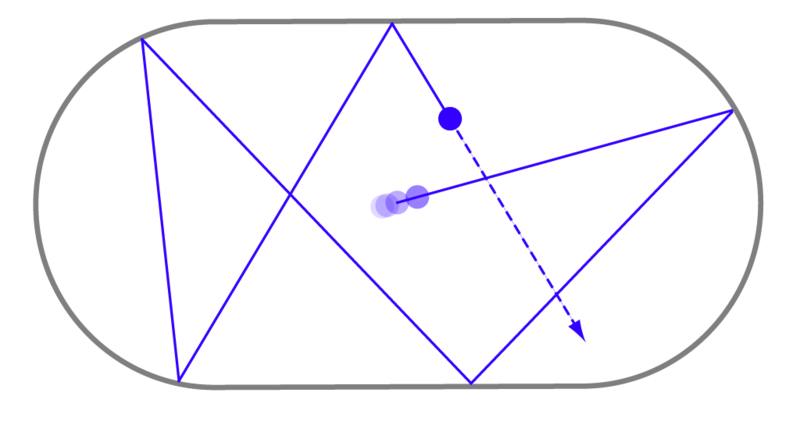
\includegraphics{figures/billiards-bunimovichstadium.png}} &
\scalebox{0.23}{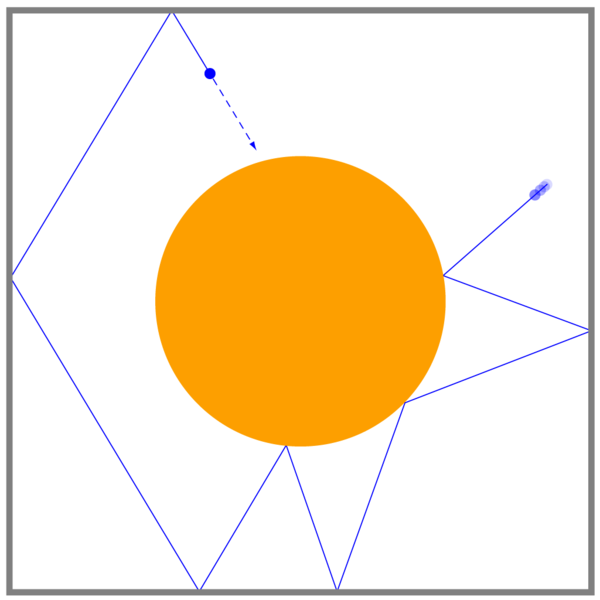
\includegraphics{figures/billiards-sinai.png}} \\  (a) & (b)
\end{tabular}
\caption{Billiard dynamical systems: (a) The ``Bunimovich stadium''; (b) The ``Sinai billiard'' (source: Wikipedia)}
\label{fig-billiards}
\end{center}
\end{figure}



The question is formulated in a deliberately vague way, but the idea behind ``ideal statistics'' is that they are represented by some probability measure $\prob$ on the phase space $\Omega$ (equipped with a suitable measurable structure $\mathcal{F}$) that is compatible with both the way the ``arbitrary'' initial state of the system is chosen, and with the action of the dynamics of the system (we shall make these ideas more precise soon). The way the observer will try to recover the measure $\prob$ is as follows: starting from the initial state $x_0$ one gets a sequence of subsequent states
$$ x_0,\ \  x_1 = T(x_0),\ \  x_2 = T(T(x_0)),\ \  x_3=T^{3}(x_0), \ldots $$
in the case of a discrete-time system, or a one-parameter family of states
$$ x_s = T_s(x_0), \qquad (s\ge 0) $$
for a continuous-time system (in both the discrete and continuous cases this would be referred to as the \textbf{orbit of $x_0$} under the dynamics). For a given event $A\in \mathcal{F}$, the observer computes the \textbf{empirical frequencies} of occurrence of $A$ in the orbit, namely
$$ \mu_A^{(n)}(x_0) = \frac{1}{n}\#\{ 1\le k\le n\,:\, x_k\in A\} = \frac1n\sum_{k=0}^{n-1}
\ind_A(x_k), \qquad (n\ge 1),
$$
or, in the case of a continuous-time system
$$
\mu_A^{(s)}(x_0) = \frac{1}{s}\int_0^s \ind_A(x_s)\,ds, \qquad (s\ge 0).
$$
One might expect that in a typical situation, the quantity $\mu_A^{(n)}(x_0)$ or its continuous-time analogue $\mu_A^{(s)}(x_0)$ should converge (as $n$ or $s$ tend to infinity) to a limit that is a constant and independent of $x_0$, except possibly for some small set of ``badly-behaved'' initial states $x_0$. If that is the case, we might denote this limit by $\prob(A)$ and say that it represents the ``ideal'' statistics of the system.

A more general way of recovering the statistics of the system is to look at \textbf{observables}, which are measurable functions $f:\Omega\to \mathbb{R}$ on the phase space (an observable is the dynamical systems or physics equivalent term for a random variable, really). For an observable $f$ we can form the \textbf{ergodic average}
$$ \mu_f^{(n)}(x_0) = \frac1n \sum_{k=0}^{n-1} f(x_k) =\frac1n \sum_{k=0}^{n-1} f(T^k(x_0)), $$
(or the analogous continuous-time quantity, whose form we leave to the reader to write down), and hope that again the ergodic averages converge to a limit, which is independent of $x_0$ and represents the ``ideal'' average value of the observable $f$, denoted $\expec(f)$ (in physics, usually this would be denoted $\langle f \rangle$). By computing this ideal average for many different observables we can recover all the information on the probability measure $\prob$.

One can now ask whether the nice situation described above actually happens in practice. Coming back to the example of billiards, it is easy to see that for some shapes of the billiard ``table'' one cannot hope to recover any meaningful statistics for the system, for what may be a trivial reason. For example, a rectangular table has the property that the ratio of the absolute values of the horizontal and vertical components of the initial speed of the ball is always preserved (equivalently, the quantity $|\tan(\alpha)|$ where $\alpha$ is the initial angle is preserved). Thus, by observing the trajectory of a single ball we have no hope of recovering any meaningful information on the statistics of the system when started with a ball for which the ``invariant'' quantity $|\tan(\alpha)|$ is different. In this case we say that the billiard dynamical system on a rectangular domain is \textbf{non-ergodic}. Less trivially, an ellipse-shaped billiard can also be shown to be non-ergodic, because of a less obvious geometric invariance property: it can be shown that an orbit will not fill the entire ellipse but will have a non-trivial envelope which is either a smaller ellipse, a hyperbola, a closed polygon or a line (see \texttt{http://cage.ugent.be/}\verb+~+\texttt{hs/billiards/billiards.html}, and Figure~\ref{fig-billiard-ellipse}).

\begin{figure}
\begin{center}
\begin{tabular}{cc}
\scalebox{0.7}{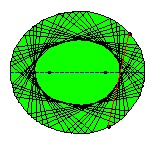
\includegraphics{figures/billiard-ellipse.jpg}} &
\scalebox{0.7}{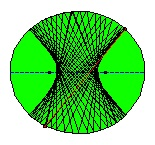
\includegraphics{figures/billiard-hyperbola.jpg}}
\end{tabular}
\caption{Billiard in an ellipse-shaped domain}
\label{fig-billiard-ellipse}
\end{center}
\end{figure}

On the other hand, in many cases, such as the domains shown in Figure~\ref{fig-billiards}, it can be proved that the nice situation exists, i.e., the billiard \emph{is} \textbf{ergodic} (we will define later what that actually means). This is related (in a way that is difficult to articulate precisely), to the emergence of a kind of ``chaos'' -- i.e., the billiard ball trajectories are erratic and irregular rather than forming a nice pattern as in the trivial examples discussed above. When ergodicity holds, the statistics of the system can be recovered from the typical trajectory of a single ball; in the case of billiards, it turns out that these statistics are quite interesting: the underlying measure $\prob$ on the phase space (which may be parametrized in terms of three parameters $\phi, \theta, \ell$ --- see the article \emph{What is the ergodic theorem?} by G.~D.~Birkhoff, \textit{American Math. Monthly}, April 1942, for the meaning of these quantities) takes the form
$$
\prob(A) = \iiint_A \frac{\sin \theta}{\sin\theta_1} \,d\theta\,d\phi\,d\ell.
$$

Note that even when the system is ergodic, there may be exceptional orbits from which one cannot recover any statistics. For example, in the Bunimovich stadium shown in Figure~\ref{fig-billiards}, a trajectory that starts in a vertical direction starting in the rectangular area bounded between the two semi-circles will be a periodic vertical line. However, the key point is that such trajectories are atypical examples that only occur on a measure 0 set of the phase space.

It should also be noted that in any given example, \emph{proving} that the ergodicity property holds may be extremely difficult. In fact, the family of dynamical systems (and even more restrictively billiard systems) for which ergodicity has been proved rigorously is quite limited, and in practical dynamical systems that one encounters in physics or other applied areas usually this is assumed without proof, as long as there is a sufficiently strong intuition that allows one to rule out a ``trivial'' reason why ergodicity should fail to hold.

In the next few sections, we shall start developing the basic ideas of ergodic theory in a more formal and precise way. The key concept is of a \textbf{measure-preserving system}, which is a probability space together with a \textbf{measure-preserving map} representing the dynamics of the system. The main result we will prove is the fundamental result of ergodic theory, known as \textbf{Birkhoff's pointwise ergodic theorem}. It explains precisely the connection between the notion of ergodicity and the ability to ``recover the statistics of the system'' as illustrated above. We shall also give some important examples and explain why the study of ergodic theory is natural from the point of view of probability theory, since one can consider the Birkhoff ergodic theorem as a powerful generalization of the strong law of large numbers.

\newpage

\lecturesamepage{Measure preserving systems}

\subsection{Measure preserving systems}

In the previous section we cheated a little bit by considering dynamical systems without an underlying measurable structure or notion of measure (in fact, such a structure was implicit in the discussion of the orbit of a ``typical'' or ``random'' initial state). In ergodic theory we concentrate on dynamical systems which come equipped with a measure, and furthermore, we require the measure to be preserved under the action of the dynamics. This idea leads to the following definitions.

\begin{defi}
Let $(\Omega, \mathcal{F}, \prob)$ be a probability space. A measurable map $T:\Omega\to\Omega$ is called \textbf{measure preserving} if for any event $E\in\mathcal{F}$ we have
\begin{equation} \label{eq:measure-pres}
\prob(T^{-1}(E)) = \prob(E).
\end{equation}
If $T$ is measure preserving, we say that the probability measure $\prob$ is \textbf{invariant under $T$}.
\end{defi}

The condition \eqref{eq:measure-pres} is sometimes written in the form $\prob=\prob\circ T^{-1}$. This can be interpreted as the statement that the push-forward of $\prob$ under $T$ is again $\prob$; that is, if $X$ is an $\Omega$-valued random variable with distribution $\prob$, then $T(X)$ has the same distribution.

\begin{defi}
A \textbf{measure preserving system} is a probability space equipped with a measure preserving map, i.e., a quadruple $(\Omega, \mathcal{F}, \prob, T)$, where $(\Omega,\mathcal{F},\prob)$ is a probability space and $T:\Omega\to\Omega$ is a measure preserving map.
\end{defi}

Measure preserving systems are the fundamental objects studied in ergodic theory (just like vector spaces are the fundamental objects of linear algebra, topological spaces are the fundamental objects of topology, etc.). It makes sense to ask to see some examples of such systems before proceeding with their theoretical study. Aside from some very interesting measure preserving systems that originate in dynamical systems (such as the billiard systems mentioned in the previous chapter), a huge class of examples arise in a very natural way in probability theory, and are intimately related to the notion of a \textbf{stationary sequence}, which is the subject of the next section.

\subsection{Stationary sequences} \label{sec-stationary}

Let $(X_n)_{n=1}^\infty$ be a sequence of random variables. The sequence is called \textbf{stationary} if for any $n,m\ge 1$, we have the equality in distribution
\begin{equation} \label{eq:def-stationary}
(X_n,\ldots,X_{n+m-1}) \stackrel{\mathcal{D}}{=} (X_1,\ldots,X_m).
\end{equation}
Note that in particular this implies that the variables $X_1,X_2,\ldots$ are identically distributed. Stationarity is a stronger property that also ensures that any pair of successive variables $(X_n,X_{n+1})$ is equal in distribution to the first pair $(X_1,X_2)$, any triple $(X_n,X_{n+1},X_{n+2})$ is equal in distribution to the first triple $(X_1,X_2,X_3)$, etc.; that is, any probabilistic question about a block of adjacent variables does not depend on the ``origin'' of the block. An i.i.d.\ sequence is a trivial example of a stationary sequence.

A stationary sequence gives rise in a natural way to a measure preserving system known as the \textbf{shift dynamics}. To define it, first note that although the variables may be defined on a generic probability space $(\Omega, \mathcal{F},\prob)$, there is no real loss of generality in assuming that the probability space is the \textbf{canonical product space}
$$ \Omega = \R^\N $$
(sometimes denoted by $\R^\infty$) together with the product $\sigma$-algebra $\mathcal{B}=\mathcal{B}(R^\N)$, and the probability measure $\mu$ defined by
$$ \mu(E) = \prob( (X_1,X_2,\ldots) \in E ), $$
(i.e., the distribution measure of the infinite-dimensional vector $(X_1,X_2,\ldots)$). In this representation, the random variables are simply the \textbf{coordinate functions}
$$ X_n(\omega) = \pi_n(\omega) = \omega_n, $$
where $\omega=(\omega_1, \omega_2, \ldots) \in \R^\N$.

On the space $(\R^\N,\mathcal{B}, \mu)$ we define the \textbf{shift map} $S:\R^\N\to\R^\N$ by
$$ S(\omega_1,\omega_2, \omega_3, \ldots) = (\omega_2,\omega_3,\omega_4, \ldots). $$

\begin{lem} The shift map $S$ is a measure preserving map of the probability space $(\R^\N,\mathcal{B},\mu)$ if and only if the sequence $(X_n)_{n=1}^\infty$ is stationary.
\label{lem-shift-stationary}
\end{lem}

\begin{exercise} Prove Lemma~\ref{lem-shift-stationary}.
\end{exercise}

\begin{defi} If $(X_n)_{n=1}^\infty$ the measure preserving system $(\R^\N,\mathcal{B},\mu,S)$ described above is called the \textbf{one-sided shift map} (or sometimes just \textbf{shift map}) associated to $(X_n)_{n=1}^\infty$.
\end{defi}

What about a two-sided shift map? One can consider a two-sided infinite sequence $(X_n)_{n=-\infty}^\infty$, and say that it is stationary if the equation \eqref{eq:def-stationary} holds for any $m\ge1$ and $n\in\Z$. One may associate with such a stationary sequence the \textbf{two-sided shift dynamics}, which is the measure preserving system $(\R^\Z,\mathcal{B}(\R^\Z), \mu, S)$, where as before $\mu$ is the distribution measure of the sequence $(X_n)_{n\in\Z}$, and $S$ is the two-sided shift, given by
$$ S((\omega_n)_{n\in\Z}) = (\omega_{n+1})_{n\in\Z}. $$
One may check easily that Lemma~\ref{lem-shift-stationary} remains true when replacing the one-sided concepts of stationary sequence and shift dynamics with their two-sided analogues.

From the definitions it may appear that the notion of a two-sided stationary sequence is more general than that of a one-sided shift, since half of the elements of a two-sided stationary sequence $(X_n)_{n\in\Z}$ can be removed to give a one-sided stationary sequence $(X_n)_{n\ge 1}$. However, in fact this is not the case, as the next result shows.

\begin{lem} Given a one-sided stationary sequence $(X_n)_{n\ge 1}$, there exists a two-sided stationary sequence $(Y_n)_{n\in\Z}$ defined on some probability space such that $(Y_n)_{n\ge1} \stackrel{\mathcal{D}}{=} (X_n)_{n\ge1}$.
\end{lem}

\begin{proof}
This is a simple example of an application of the Kolmogorov extension theorem, a useful result from measure theory that enables one to construct measures on infinite product spaces with prescribed finite-dimensional marginals (see [Dur2010], section A.3). Here, the stationarity condition \eqref{eq:def-stationary} determines the joint $m$-dimensional distribution of any block $(Y_n,\ldots,Y_{n+m-1})$ of $m$ successive random variables in the sequence, where $m\ge1$ and $n\in\Z$. These distributions satisfy the consistency condition in the Kolmogorov extension theorem, and therefore are indeed the $m$-dimensional marginals of some infinite sequence $(Y_n)_{n\in\Z}$ defined on a single probability space.
\end{proof}

We saw that we can associate with any stationary sequence a measure preserving system. Going in the opposite direction, if we start with a measure preserving system $(\Omega, \mathcal{F}, \prob, T)$, any random variable $X:\Omega\to\R$ (what we called an \emph{observable} in the previous chapter) can be transformed by $T$ to a new variable
$$ X\circ T = X(T). $$
The measure preserving property implies that $X\circ T$ is equal in distribution to $X$. By starting with $X$ and repeatedly iterating the transformation $T$ we get a sequence $(X_n)_{n=1}^\infty$ given by
$$ X_n = X\circ T^{n-1}. $$

\begin{lem} \label{lem-mps-stationary}
$(X_n)_n$ is a stationary sequence.
\end{lem}

\begin{exercise}
Prove Lemma~\ref{lem-mps-stationary}
\end{exercise}

The conclusion from the above discussion is that the study of stationary sequences is roughly equivalent to the study of measure preserving systems with a distinguished observable, and indeed much of ergodic theory could be developed using just the language of stationary sequences, although this would come at great cost to the elegance and beauty of the theory.

\subsection{Examples of measure preserving systems}

\begin{enumerate}[1.]
\item \textbf{i.i.d.\ sequences.} As mentioned in the previous section, any i.i.d.\ sequence is stationary and hence has an associated shift measure preserving system, referred to as an \textbf{i.i.d.\ shift}. In the case when the i.i.d.\ random variables take on only a finite number of values with positive probability this measure preserving system is known as a \textbf{Bernoulli shift}.
\item \textbf{A shift-equivariant function of a stationary sequence.} Given a stationary sequence $(X_n)_{n=1}^\infty$ and a measurable function $F:\R^\N\to\R^\N$ one can manufacture a new stationary sequence $(Y_n)_{n=1}^\infty$ via the equation
\begin{equation} \label{eq:shift-equivariant} 
Y_n = F(X_n,X_{n+1},X_{n+2},\ldots), \qquad (n\ge 1).
\end{equation}
The verification that $(Y_n)_n$ is stationary is easy and is left to the reader. In this way one can generate starting from a known stationary sequence (e.g., an i.i.d.\ sequence) a large class of new and interesting sequences.
\item \textbf{Stationary finite-state Markov chains.} Let $A=\{\alpha_1,\ldots,\alpha_d\}$ be a finite set. A \textbf{finite-state Markov chain with state space $A$} is a sequence $(X_n)_{n=0}^\infty$ of $A$-valued random variables such that for each $n\ge0$ and $1\le j_1,j_2,\ldots,j_{n+1}\le d$ we have that
\begin{equation} \label{eq:markov-property}
\prob(X_{n+1} = \alpha_{j_{n+1}}\,|\,X_1=\alpha_1,\ldots,X_n=\alpha_n)
=
\prob(X_{n+1} = \alpha_{j_{n+1}}\,|\,X_n=\alpha_n).
\end{equation}
That is, the conditional distribution of $X_{n+1}$ given the $n$ preceding values $X_1,\ldots,X_n$ is only dependent on the value of the last observed variable $X_n$; this property is known as the \textbf{Markov property}. In most cases the chain is also assumed to be \textbf{time-homogoneous}, meaning that the expression in \eqref{eq:markov-property} is independent of $n$. In this case, if we denote
$$ p_{i,j} = \prob(X_{2} = \alpha_j\,|\,X_1=\alpha_i), \qquad (1\le i,j\le d), $$
then the matrix $P = (p_{i,j})_{i,j=1}^d$ together with the probability distribution of the initial state $X_0$ determine the distribution of the entire sequence. The probability $p_{i,j}$ is referred to as the \textbf{transition probability from state $i$ to $j$}, and the matrix $P$ is called the \textbf{transition matrix} of the chain. The distribution of $X_0$ is usually given as a probability vector $\pi=(\pi_1,\ldots,\pi_d)$ where $\pi_j=\prob(X_0=j)$. It is easy to show (we will do so later, when we study Markov chains more in depth) that the vector $\pi^{(n)} = (\pi_1^{(n)},\ldots,\pi_d^{(n)})$ representing the probability distribution of $X_n$ is obtained from $\pi$ and $P$ via
$$ \pi^{(n)} = \pi P^n, $$
the linear-algebraic result of multiplying the row vector $\pi$ by the matrix $P$ multiplied by itself $n$ times.

Assume now that $\pi$ is chosen to be a probability vector satisfying the equation $\pi=\pi P$; i.e., $\pi$ is a left-eigenvector of the transition matrix $P$ with eigenvalue $1$. By the above remarks, this means that the sequence $(X_n)_n$ is a sequence of identically distributed random variables, and furthermore it is easy to see that $(X_n)_n$ is in fact a stationary sequence. A Markov chain started with such an initial state distribution is called a \textbf{stationary Markov chain}. The associated shift measure preserving system is known as a \textbf{Markov shift}.

\item \textbf{Tossing a randomly chosen coin.} Let $0\le U\le 1$ be a random variable. We can define a stationary sequence $X_1,X_2,\ldots$ by the following ``two-step experiment'': first, pick a random coin with bias $U$; then, toss the chosen coin infinitely many times (the coin tosses being independent of each other), denoting the results (encoded as 0's or 1's) by $X_1,X_2,\ldots$. Formally, we can define the distribution of the sequence by
$$ 
\prob(X_1=a_1,\ldots,X_n=a_n) = \expec\left[U^{\sum_j a_j} (1-U)^{n-\sum_j a_j}\right], \qquad a_1,\ldots,a_n\in\{0,1\}.
$$
Note that the $X_n$'s are identically distributed (in fact, the sequence is stationary), but \emph{not} independent (except in the extreme case when $U$ is a.s.\ constant); rather, they are said to be conditionally independent given $U$.

\item \textbf{P\'olya's urn experiment.} Let $I_n$ be as in Chapter~1 the indicator random variable of the event that in P\'olya's urn experiment a white ball was drawn in the $n$th round. We proved that the distribution of the sequence $(I_n)_{n=1}^\infty$ is invariant under finite permutations, so in particular it is stationary and has an associated measure preserving shift.

\item \textbf{Rotation of the circle} (a.k.a.\ \textbf{$x+\alpha$ modulo 1}).
Let $(\Omega,\mathcal{F},\prob)$ be the unit interval $[0,1]$ with Lebesgue measure. One can consider $[0,1]$ to be topologically a circle by identifying both endpoints $0$ and $1$ as a single point. Fix $0\le \alpha<1$. The \textbf{circle rotation map} $R_\alpha:[0,1)\to[0,1)$, which rotates the circle by a fraction $\alpha$, is defined by
$$ R_\alpha(x) = x+\alpha \textrm{\ mod\ } 1 = \begin{cases} x+\alpha & \textrm{if }x+\alpha<1, \\ x+\alpha-1&\textrm{otherwise}. \end{cases}
$$
\begin{lem}
$R_\alpha$ preserves Lebesgue measure.
\end{lem}

\begin{proof} If $A\subset [0,1]$ is a Borel set, then
\begin{align*}
\operatorname{Leb}(R_\alpha^{-1}(A)) &= 
\operatorname{Leb}\Big( \big(A\cap[0,\alpha)+1\big) \sqcup \big(A\cap[\alpha,1)-1\big) \Big)
\\ &=
\operatorname{Leb}\big(A\cap[0,\alpha)+1\big) 
+  \operatorname{Leb}\big(A\cap[\alpha,1)-1\big) \\ &=
\operatorname{Leb}\big(A\cap[0,\alpha)\big) 
+  \operatorname{Leb}\big(A\cap[\alpha,1)\big) \\ &=
\operatorname{Leb}\Big( \big(A\cap[0,\alpha)\big) \sqcup \big(A\cap[\alpha,1)\big) \Big)
=
\operatorname{Leb}(A).
\end{align*}
\end{proof}


\item \textbf{The $2x$~mod~$1$ map.} Similarly to the previous example, the \textbf{$2x$~mod~$1$ map} or \textbf{doubling map} is also defined on the probability space $[0,1]$ with Lebesgue measure, and is given by
$$ D(x) = 2x\textrm{ mod }1 = \begin{cases} 2x&x<\tfrac12, \\ 2x-1&x\ge\tfrac12. \end{cases}
$$

\begin{lem}
$D$ preserves Lebesgue measure.
\end{lem}

\begin{proof} If $A\subset [0,1]$ is a Borel set, then
$$ \operatorname{Leb}(D^{-1}(A)) = 
 \operatorname{Leb}\left(\tfrac12 A \sqcup \left(\tfrac12 A+\tfrac12\right) \right)
 = \tfrac12 \operatorname{Leb}(A)
 + \tfrac12 \operatorname{Leb}(\tfrac12+A) =
\operatorname{Leb}(A).
$$
\end{proof}

We have seen before that the measure space $[0,1]$ with Lebesgue measure is isomorphic to the product space of an infinite sequence of i.i.d.\ unbiased coin tosses. It is easy to see that under this isomorphism, the doubling map translates to the shift map $S$ of the Bernoulli sequence. So, the doubling map is really a disguised version of the Bernoulli shift associated with i.i.d.\ unbiased coin tosses.

\item \textbf{The continued fraction map.} A well-known fact from number theory says that any
rational number $x\in (0,1)$ has a unique \textbf{continued fraction expansion} of the form
$$ x = \frac{1}{n_1+\frac{1}{n_2+\frac{1}{n_3+\frac{1}{\ddots+\frac{1}{n_k}}}}},
$$
where $k\ge 1$, $n_1,\ldots,n_k\in \N$ and $n_k>1$. Such an expansion is said to be finite, or terminating. Similarly,
any irrational $x\in(0,1)$ has a unique \emph{infinite} continued fraction expansion, which takes the form
$$ x = \frac{1}{n_1+\frac{1}{n_2+\frac{1}{n_3+\frac{1}{n_4+\frac{1}{\ldots}}}}},
$$
where $n_1,n_2,n_3\ldots \in \N$. The numbers $n_1,n_2,\ldots$ are called the \textbf{quotients} of the expansion, and are analogous to the digits in the decimal (or base-$b$) expansion of a real number. They are computed using a process that is a natural generalization of the Euclidean algorithm to real numbers, namely:
\begin{align*}
n_1 &= \textrm{the number of times a stick of length $x$ ``fits'' inside a stick of length $1$}, \\
n_2 &= \textrm{the number of times a stick of length $x_2=(1-n_1x)$ fits inside a stick}\\ &\ \ \ \ \textrm{of length $x$},
\\
n_3 &= \textrm{the number of times a stick of length $x_3=(x-n_2x_1)$ fits inside a stick}
\\ &\ \ \ \ \textrm{of length $x_2$}, \\
& \ \,\vdots
\end{align*}
Gauss studied in 1812 the statistical distribution of the quotients for a number $x$ chosen uniformly at random in $(0,1)$. In this case, since $x$ is irrational with probability~$1$ we need not worry about terminating expansions, and can consider the quotients $n_1, n_2, \ldots$ to be random variables defined on the measure space $(0,1)$ equipped with Lebesgue measure. Gauss reformulated the problem in terms of a measure preserving system (before this concept even existed!) now called the \textbf{continued fraction map} or \textbf{Gauss map}. To see how this reformulation works, note first that, in the computation above, the first quotient $n_1$ can be represented in the form
$$ n_1 = \left\lfloor \frac{1}{x} \right\rfloor $$
(where $\lfloor z \rfloor$ denotes as usual the integer part of a real number $z$). Next, observe that, to continue with the computation of the next quotients $n_2,n_3,\ldots$, instead of replacing the two yardsticks of lengths $1$ and $x$ (which are used in the computation of the first quotient $n_1$) by a pair of yardsticks of lengths $x$ and $x_2=1-n_1 x$, one can instead rescale the yardstick of length $x$ to be of length 1, so that the yardstick of length $x_2$ becomes of length
$$ x'=\frac{1-n_1 x}{x} = \frac{1}{x}-n_1 = \left\{ \frac{1}{x} \right\} $$
(where $\{z\}=z-\lfloor z\rfloor$ is the \textbf{fractional part} of $z$). The quotient $n_2$ can be computed from this rescaled value $x'$ in the same way that $n_1$ is computed from $x$. By continuing in this way one can obtain all the quotients by successive rescaling operations. Formally, define the Gauss map $G:(0,1)\to[0,1)$ and a function $N:(0,1)\to\N$ by
$$
G(x) = \left\{ \frac{1}{x}\right\}, \qquad
N(x) = \left\lfloor \frac{1}{x}\right\rfloor. 
$$
Then the above comments show that the quotients $n_1,n_2,\ldots$ are obtained by
\begin{align*}
n_1 &= N(x), \\
n_2 &= N(G(x)), \\
n_3 &= N(G^2(x)), \ \ldots \\
n_k &= N(G^{k-1}(x)), \ \ldots 
\end{align*}

(Note that the range of $G$ is $[0,1)$ instead of the open interval $(0,1)$ since $G(x)=0$ exactly when $x$ is a rational number of the form $x=1/m$; this is related to the fact that if we start with any rational number $x$, after a finite number of iterations of $G$ we will reach $0$ and will not be able to extract any more quotients.)

If you guessed that the Gauss map $G$ preserves Lebesgue measure, you guessed wrong. The real situation is more interesting:

\begin{lem} \label{lem-gauss-measure}
The map $G$ preserves the \textbf{Gauss measure} $\gamma$ on $(0,1)$, given by
$$ \gamma(A) = \frac{1}{\log 2} \int_A \frac{dx}{1+x}. $$
\end{lem}

\begin{exercise} Prove Lemma~\ref{lem-gauss-measure}.
\end{exercise}


%\begin{proof} *** ADD THIS ***
%\end{proof}

An important observation is that Gauss measure and Lebesgue measure are mutually absolutely continuous with respect to each other. This means that any event which has probability $1$ with respect to one is also a probability 1 event with respect to the other. Thus any almost-sure statistical results about the measure preserving system $((0,1),\mathcal{B},\gamma,G)$ (which will be obtained from the Birkhoff ergodic theorem once we develop the theory a bit more) will translate immediately to statements about the behavior of the continued fraction expansion of a \emph{uniformly random} real number.

The continued fraction map described above is intimately related to the Euclidean algorithm for computing the greatest common divisor (GCD) of two integers, since iterating the map starting from a rational fraction $p/q$ reproduces precisely the sequence of quotients (and remainders, if one takes care to record them) in the execution of the Euclidean algorithm, and the last non-zero iteration $T^k(p/q)$ is of the form $1/d$, where $d$ is precisely the GCD of $p$ and $q$. Given the usefulness of the Euclidean algorithm and its historical status as one of the earliest algorithms ever described, is not surprising that already in the early days of the theory of algorithms (a.k.a.\ the 1960's) researchers were interested in giving a quantitative analysis of the running time of this venerable procedure. Such analyses lead directly to ergodic theoretic questions about the continued fraction map; the renewed interest in this classical problem has stimulated new and extremely interesting studies into the mathematics of the Gauss map. A highly readable account of these fascinating developments (the latest of which being less than 15 years old and still inspiring new research even in recent years) is told in Sections~4.5.2--4.5.3 of Vol.~II of Donald E.\ Knuth's celebrated book series \emph{The Art of Computer Programming}.

\item \textbf{The binary GCD algorithm.} Continuing the discussion above, a fact that is little-known outside computer science circles is that in modern times a new algorithm for computing GCD's was proposed that gives the Euclidean algorithm a serious run for its money, and is actually faster in some implementations. This algorithm was proposed by Josef Stein in 1967 and is known as \textbf{the binary GCD algorithm} or \textbf{Stein's algorithm}. It replaces the integer division operations of the Euclidean algorithm, which are costly in some computer architectures, with a clever use of subtractions (which are generally cheap) and divisions by 2, which can be implemented in machine language as (also cheap) bit shift operations. 

[Here is a summary of the algorithm: start with two integers $u<v$. First, extract the common power-of-$2$ factor to get to a situation where at least one of $u,v$ is odd. Then, successively replace $(u,v)$ with the new pair $(v-u)/2^k,u$ (sorted so that the smaller one gets called ``$u$'' and the bigger one ``$v$''), where $2^k$ is the maximal power of 2 dividing $v-u$. Eventually one of the numbers becomes $0$ and the remaining one represents the odd component of the GCD of the original numbers.]

The computer scientist Richard Brent noticed in 1976 that this algorithm can also be reformulated in terms of a dynamical system.
Similarly to the case of the Euclidean algorithm, the theoretical analysis of the running time of the binary GCD algorithm leads to highly nontrivial questions (most of them still open) about the behavior of this dynamical system. In particular, this system has an invariant measure that is mutually absolutely continuous with respect to Lebesgue measure, and is analogous to the Gauss measure, but no good formula for it is known. See Section~4.5.3 in Knuth's book mentioned above for more details.

\item \textbf{The $3x+1$ map.} The \textbf{3x+1 problem} or \textbf{Collatz problem} is a famous open problem (studied since the 1950's, and originating in work of L.~Collatz around 1932) about a discrete dynamical system on the positive integers. It pertains to iterations of the map $T:\N\to\N$ defined by
$$ T(n) = \begin{cases} 3n+1 & \textrm{if $n$ is odd}, \\ \frac{\displaystyle n}{\displaystyle 2} & \textrm{if $n$ is even}.
\end{cases}
$$
The conjecture is that for any initial number $n_0$, iterating the map will eventually lead to the cycle $1,4,2,1,4,2,1,\ldots$ The mathematician Paul Erd\"os was quoted as saying ``Mathematics is not yet ready for such problems'' and offered a $\$500$ prize for its solution.

One of the many (ultimately unsuccessful) attempts to study the problem was based on the beautiful observation that this dynamical system can be turned into a measure preserving system, by extending its domain of definition to the ring $\textbf{Z}_2$ of \textbf{$2$-adic integers}. This is an extension of the usual ring $\Z$ of integers in which every element has a binary expansion that extends \emph{infinitely far to the left} (instead of to the right as a real number would). That is, a dyadic integer is a formal expression of the form
$$ a_0 + 2\cdot a_1 + 4\cdot a_2 + 8\cdot a_3 + \ldots + 2^n a_n + \ldots = \sum_{n=0}^\infty a_n 2^n
$$
where $a_0,a_1,a_2,\ldots\in \{0,1\}$.
It can be shown that one can do algebra, and even an exotic form of calculus, on these numbers (and more generally over similar sets of numbers in which the binary expansion is replaced by a base-$p$ expansion where $p$ is an arbitrary prime number --- these are the so-called \textbf{$p$-adic integers}). Since the notion of the parity of a number extends to $2$-adic integers, the $3x+1$ map $T$ extends in an obvious way to a map $\tilde{T}:\mathbf{Z}_2\to\mathbf{Z}_2$. It can be shown that $\tilde{T}$ preserves the natural volume measure of $\textbf{Z}_2$. For more information, see Wikipedia or the article \emph{The $3x+1$ problem and its generalizations}, by J.~C.~Lagarias (\textit{American Math. Monthly} 92 (1985), 3--23).


\item \textbf{Billiards.} In Chapter~5 we discussed billiard dynamical systems, and mentioned a formula on the limiting statistics of such a system, in the case when it is ergodic. This is related to the fact that the billiard dynamics also has an invariant measure, given (in a suitable parametrization of the phase space) by
$$
\mu(A) = \iiint_A \frac{\sin \theta}{\sin\theta_1} \,d\theta\,d\phi\,d\ell.
$$

\item \textbf{Hamiltonian flow.} \textbf{Hamiltonian mechanics} is a formalism for modeling a mechanical system of particles and rigid bodies interacting via physical forces, with no external influences. The phase space is some set $\Omega$ representing the possible states of the system (formally, it is a \textbf{symplectic manifold}, and has a smooth structure --- i.e.,  one can solve differential equations on it and do other calculus-type operations). The \textbf{Hamiltonian flow} is a semigroup of maps $(H_s)_{s\ge 0}$ representing the time-evolution of the system, i.e., $H_s(\omega)$ takes an initial state $\omega\in\Omega$ of the system and returns a new state representing the state of the system $s$ time units in the future. A result known as Liouville's theorem says that the natural volume measure of the manifold is preserved under the Hamiltonian system. Thus, the Hamiltonian flow is a \textbf{measure preserving flow} (the continuous-time analogue of a measure preserving system, which we will not discuss in detail). Such flows provided some of the original motivation for questions of ergodic theory, since, e.g., statistical physicists in the 19th century wanted to understand the statistical behavior of ideal gases (note that billiard can be thought of a toy model for a gas in an enclosed region).

\item \textbf{Geodesic flow.} On a compact Riemann surface (or more generally a Riemannian manifold), the geodesic flow $(\varphi_s)_{s\ge0}$ is a family of maps, where each $\varphi_s$ takes a point on the manifold together with a ``direction'' at $s$ (formally, an element of the tangent space at $s$), and returns a new pair ``point+direction'' that is obtained by proceeding $s$ units of distance along the unique geodesic curve originating from $s$ in the given direction. (For a more formal description, see Wikipedia or a textbook on differential geometry). The geodesic flow preserves the volume measure and is thus a measure preserving flow.

\item \textbf{The logistic map.} The logistic map was originally studied as a simple model for the dynamics of population growth of animal and plant species. It is given by the formula
$$ L_r(x) = rx(1-x) \qquad (0<x<1),$$
where $r>0$ is a parameter of the system. Here, $x$ represents the size of the population, and $L_r(x)$ represents the size of the population one generation later, so successive iterations $L_r^{n}(x)$ correspond to the evolution of the population sizes over time starting from some initial size $x$. The assumptions underlying the model are that when $x$ is small one should observe roughly exponential growth when iterating the map, but as the size of the population increases, the environmental resources required to support growth are depleted, leading to starvation and a sharp decrease in the population size.

The logistic map is a famous example of the emergence of \textbf{chaos}: for values of $r$ between $0$ and $3$, the system stabilizes around a unique value ($0$ if $r\le 1$, or $(r-1)/r$ if $1\le r\le 3$). When $r$ becomes slightly bigger than 3 a \textbf{bifurcation} occurs, leading to an oscillation between 2 values; as $r$ increases further, additional bifurcations occur (oscillation betweeen 4 values, 8 values etc.) until chaotic behavior emerges at $r\approx 3.57$  and continues (with occasional intervals of stability) until $r=4$, after which point the range of the map leaves $[0,1]$ so the model stops making sense as a dynamical system. See Figure~\ref{fig-logistic-chaos} for an illustration of this remarkable phenomenon.

\begin{figure}
\begin{center}
\scalebox{0.4}{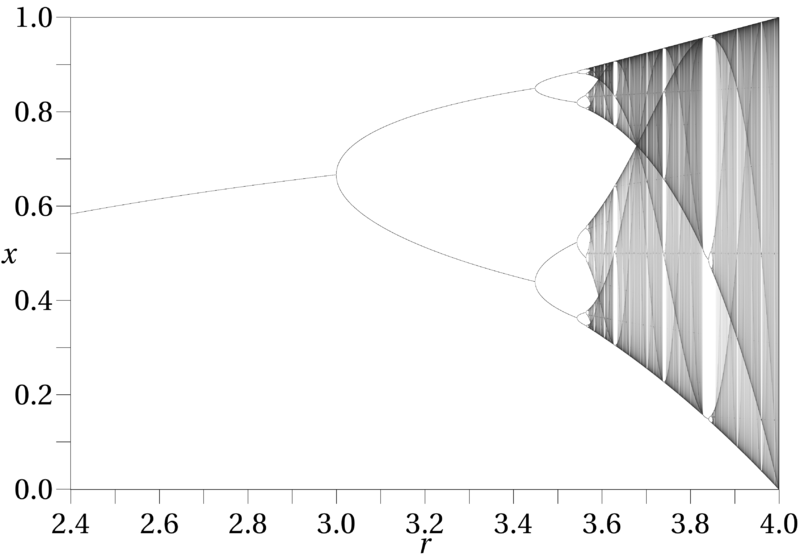
\includegraphics{figures/logisticmap.png}}
\caption{Chaos in the logistic map (source: Wikipedia)}
\label{fig-logistic-chaos}
\end{center}
\end{figure}

\begin{lem} \label{lem-logistic-invariant}
When $r=4$, the map $L_4$ has an invariant measure $\lambda$ on $(0,1)$ given by
$$ \lambda(dx) = \frac{1}{\pi \sqrt{x(1-x)}}\,dx $$
(also known as the $\operatorname{Beta}(\tfrac12,\tfrac12)$ distribution).
\end{lem}

\begin{exercise} Prove Lemma~\ref{lem-logistic-invariant}
\end{exercise}



\end{enumerate}


\subsection{Ergodicity}

Let $(\Omega, \mathcal{F}, \prob, T)$ be a measure preserving system. An event $A\in\mathcal{F}$ is called \textbf{$T$-invariant} (or \textbf{invariant under $T$}, or just \textbf{invariant} if the context is clear) if $$ T^{-1}(A) = A \ \ \textrm{a.s.}, $$
with the convention that two events $A,B$ are considered equal almost surely if their symmetric difference has probability $0$. That is, $A$ is invariant if
$$ \prob(A\triangle T^{-1}(A)) = 0, $$
(where $A\triangle B = (A\setminus B)\cup (B\setminus A)$ denotes the symmetric difference of two sets).
We denote by $\mathcal{I}$ the collection of a.s.\ invariant events.

\begin{lem} \label{lem-invariant-sigmaalg}
$\mathcal{I}$ is a $\sigma$-algebra.
\end{lem}

\begin{exercise}
Prove Lemma~\ref{lem-invariant-sigmaalg}.
\end{exercise}

\begin{defi} The measure preserving system $(\Omega, \mathcal{F}, \prob, T)$ is called \textbf{ergodic} if for any invariant event $A$, $\prob(A)=0$ or $\prob(A)=1$.
\end{defi}

A sub-$\sigma$-algebra of $\mathcal{F}$ all of whose events have probability 0 or 1 is called \textbf{trivial}. (We already saw an example: the $\sigma$-algebra of tail events of an i.i.d.\ sequence of random variables is trivial, according to the Kolmogorov 0-1 law.) So, another way of saying that a measure preserving system is ergodic is that its $\sigma$-algebra $\mathcal{I}$ of invariant events is trivial.

There is an equivalent way to characterize ergodicity in terms of invariant random variables rather than events, given in the following exercise.

\begin{exercise} If $(\Omega, \mathcal{F}, \prob, T)$ is a measure preserving system, a random variable $X:\Omega\to\R$ is called \textbf{invariant} if $X\circ T \equiv X$ almost surely. Prove that a random variable is invariant if and only if it is measurable with respect to $\mathcal{I}$, and that a system is ergodic if and only the only invariant random variables are almost surely constant.
\end{exercise}

\begin{exercise} Show that a measure preserving system $(\Omega, \mathcal{F}, \prob, T)$ is ergodic if and only if the probability measure $\prob$ \emph{cannot} be represented in the form
$$ \prob = \alpha Q_1 + (1-\alpha)Q_2, $$
where $0<\alpha<1$ and $Q_1, Q_2$ are two distinct $T$-invariant probability measures on the measurable space $(\Omega, \mathcal{F})$. (In words, this means that an ergodic system cannot be decomposed into a nontrivial convex combination of two simpler systems.)
\end{exercise}



To get a feel for this new concept, let us examine which of the measure preserving systems discussed in the previous section are ergodic.

\begin{enumerate}[1.]
\item \textbf{i.i.d.\ sequence.} Let $A$ be an invariant event in the i.i.d.\ shift. $A$ is in the product $\sigma$-algebra, in other words, it is measurable with respect to $\sigma(X_1,X_2,\ldots)$, where $X_1,X_2,\ldots$ denote the coordinate functions of the product space. Then
$$ S^{-1}(A) = \{ \omega\in \R^\N \, : \, (\omega_2,\omega_3,\ldots) \in A \} $$
is measurable with respect to $\sigma(X_2,X_3,\ldots)$, and similarly, for any $n\ge 1$,
$$ S^{-n}(A) = \{ \omega\in \R^\N \, : \, (\omega_{n+1},\omega_{n+2},\ldots) \in A \} $$
is in $\sigma(X_{n+1},X_{n+2},\ldots)$. It follows that
$$ A'=\bigcap_{N=1}^\infty \bigcup_{n=N}^\infty S^{-n}(A) = \{ S^{-n}(A) \textrm{ i.o.} \} $$
is a tail event, and hence has probability $0$ or $1$ by the Kolmogorov 0-1 law. But we assumed that $A$ was invariant, which implies that $A=S^{-n}(A)$ almost surely for all $n\ge 1$, and therefore also $A=A'$ almost surely. It follows that $A$ is also a 0-1 event\footnote{The above argument shows that $\mathcal{I}\subseteq\mathcal{T}$ (the $\sigma$-algebra of invariant subsets is contained in the tail $\sigma$-algebra), as long as we identify sets which are a.s.\ equal.
}. We have proved:

\begin{lem} \label{lem-iid-ergodic} Any i.i.d.\ shift map is ergodic.
\end{lem}

\item \textbf{A shift-equivariant function of an ergodic stationary sequence.}\footnote{In more abstract treatments of ergodic theory, this example would be called a \textbf{factor map} or \textbf{homomorphism}. An important family of problems in ergodic theory is concerned with identifying when one measure preserving system can be obtained as a homomorphism of another (usually simpler) measure preserving system, and especially when one can find an \emph{invertible} homomorphism, also known as an \textbf{isomorphism}, between the two systems.} Let $(X_n)_n$ be a stationary sequence whose associated shift system is ergodic (such a sequence is called simply a \textbf{stationary ergodic sequence}), and let $Y_n$ be defined as in \eqref{eq:shift-equivariant}.

\begin{lem} The stationary sequence $(Y_n)_n$ is also ergodic.
\end{lem}

\begin{proof}
Let $A$ be an invariant event for the $(Y_n)$ sequence. We can think of $A$ as ``living'' in the original product space $\R^\N$ associated with the shift map for the sequence $(X_n)_n$. (Formally, the sequence $(Y_n)_n$ is an infinite-dimensional random vector, i.e., it maps the $\R^\N$ ``of'' the $(X_n)_n$ sequence into a ``different copy'' of $\R^\N$; by pulling back the event $A$ with respect to this mapping we get a ``copy'' of $A$ in the original product space.) The fact that $A$ is invariant under shifting the $Y_n$'s means it is also invariant under the original shift of the $X_n$'s, hence is a 0-1 event by the assumption that the $(X_n)_n$ sequence is ergodic.
\end{proof}



\item \textbf{Stationary finite-state Markov chains.} A Markov chain is called \textbf{irreducible} if any state can be reached in a sequence of steps from any other state. It is not hard to prove (see [Dur2010, Example~7.1.7, p.~281]) that a stationary finite-state Markov chain is ergodic if and only if it is irreducible.

\item \textbf{Tossing a randomly chosen coin.} In this experiment we have
$$ U = \lim_{n\to\infty} \frac{1}{n}\sum_{k=1}^n X_k $$
by the strong law of large numbers (conditioned on the value of $U$). So, the random coin bias $U$ is an invariant random variable, and thus the sequence $(X_n)_n$ is ergodic if and only if $U$ is a.s.\ constant (equivalently, if and only if the sequence is i.i.d.).

We should note that this process is in some sense an archetypical example of a non-ergodic process, in the sense that non-ergodicity is precisely the behavior in which the experiment chooses ``at the dawn of time'' some random data or information (represented by the $\sigma$-algebra of invariant events), and then performs a stationary ergodic sequence of experiments that depends on this initial data. In other words, a general stationary sequence can always be represented as a mixture, or a kind of weighted average, of stationary ergodic sequences, where the weights in the mixture correspond to the probability distribution of the initial data. (The precise formulation of this statement leads to the concept of the \textbf{ergodic decomposition} of a measure preserving system, which we will not discuss in detail since it requires some slightly advanced notions from functional analysis.)

\begin{exercise}
Show that the $\sigma$-algebra $\mathcal{I}$ of invariant subsets for this process coincides with the $\sigma$-algebra $\sigma(U)$ generated by the random coin bias $U$. That means that, not only is $U$ an invariant random variable, but any other invariant random variable can be computed once the value of $U$ is known.
\end{exercise}

\item \textbf{P\'olya's urn.} The limiting fraction $Y$ of white balls in the urn (see \eqref{eq:polya-as-conv}) is an invariant random variable. By \eqref{eq:polya-beta-dist}, it is non-constant, which shows that the shift associated  with the stationary sequence of indicators $(I_n)_n$ in P\'olya's urn experiment is not ergodic.

It is an amusing and rather counter-intuitive fact that the P\'olya urn experiment is actually a special case of the ``tossing a randomly chosen coin'' family of examples discussed above. In fact, the ``random coin bias'' $U$ is equal to the limiting fraction $Y$ of white balls in the urn. To see this, note that by a short computation \eqref{eq:polyaurn-formula} can be massaged into the form
$$ \prob(I_1=x_1, \ldots, I_n=x_n) = \frac{B(a+k, b+n-k)}{B(a,b)}, $$
where $B(u,v)=\int_0^1 x^{u-1}(1-x)^{v-1}\,dx$ denotes the Euler beta function, and $k=\sum_{j=1}^n x_j$ (check!). We can further recognize the quantity on the right hand side as an expectation, namely
$$ \frac{B(a+k, b+n-k)}{B(a,b)}= \frac{1}{B(a,b)}\int_0^1 x^{a-1}(1-x)^{b-1} x^k(1-x)^{n-k}\,dx = \expec(U^k(1-U)^{n-k}), $$
where $U\sim \operatorname{Beta}(a,b)$. Thus, we have the amazing fact that, in effect, P\'olya's urn behaves as if at the beginning of time, it \emph{chooses} the random limiting fraction $Y$ of white balls (without telling the experimenter!), and subsequently tosses an i.i.d.\ sequence of coin tosses with bias $Y$ to choose the successive colors of the balls that get added to the urn. Furthermore, by the exercise above, the $\sigma$-algebra of invariant subsets is the one generated by $Y$, so intuitively one can say that this random variable measures the precise extent of non-ergodicity in the process, i.e., the decomposition of the process into its ergodic components.

\item \textbf{Rotation of the circle.} The following result has a natural number theoretic interpretation, which we'll discuss later after proving the Birkhoff pointwise ergodic theorem.
\begin{thm} The circle rotation map $R_\alpha$ is ergodic if and only if $\alpha$ is irrational.
\end{thm}

\begin{proof} If $\alpha=p/q$ is rational, the set 
$$ E = \left[0, \tfrac{1}{2q}\right]
\cup \left[\tfrac{1}{q}, \tfrac{3}{2q}\right] 
\cup \left[\tfrac{2}{q}, \tfrac{5}{2q}\right] 
\cup \left[\tfrac{3}{q}, \tfrac{7}{2q}\right] 
\cup \ldots
\cup \left[\tfrac{q-1}{q}, \tfrac{2q-1}{2q}\right]
$$
is an example of a nontrivial invariant set. Conversely, assume that $\alpha$ is irrational. Let $A \subset [0,1]$ be an invariant event. The indicator variable $\ind_A$ is a bounded measurable function, hence an element of $L_2[0,1]$, and can therefore be expanded in the Fourier basis
$$ \ind_A(x) = \sum_{n=-\infty}^\infty c_n e^{2\pi inx}. $$
(The equation represents an equality in $L_2$, i.e., it is true for almost every $x\in [0,1]$.) The coefficients $c_n$ in the expansion are given by
$c_n = \frac{1}{2\pi} \int_0^1 \ind_A(x) e^{-2\pi i n x}\,dx$.
 Then we have
\begin{align*}
\ind_{R_\alpha^{-1}(A)}(x) &= (\ind_A\circ R_\alpha)(x) = \ind_A(R_\alpha(x))
= \sum_{n=-\infty}^\infty c_n e^{2\pi i n R_\alpha(x)}
= \sum_{n=-\infty}^\infty c_n e^{2\pi i n (x+\alpha\textrm{ mod }1)}
\\ &
= \sum_{n=-\infty}^\infty c_n e^{2\pi i n (x+\alpha)}
= \sum_{n=-\infty}^\infty d_n  e^{2\pi i n x},
\end{align*}
where we denote $d_n = c_n e^{2\pi in\alpha}$. Since $A$ is invariant, i.e., $\ind_{R_\alpha^{-1}(A)}=\ind_A$ a.s., we get that $c_n=d_n$ for all $n\in\Z$. But $\alpha$ is irrational, so $e^{2\pi in\alpha}\neq 1$ if $n\neq 0$. It follows that $c_n=0$ for all $n\neq 0$, which leaves only the constant Fourier coefficient, i.e.,
$ \ind_A \equiv c_0$ a.s., which proves that $A$ is a trivial event.
\end{proof}


\item \textbf{The $2x\textrm{ mod }1$ map.} As we discussed earlier, this system is equivalent to the $(\tfrac12,\tfrac12)$ Bernoulli shift, so by Lemma~\ref{lem-iid-ergodic} above, the doubling map is ergodic.

\item \textbf{The continued fraction map.} The Gauss map is ergodic, a fact which has important consequences (which we will discuss in the next chapter) for understanding the distribution of continued fraction quotients of a typical real number. There are many proofs of this result. See for example the book \textit{Ergodic Theory and Information} by P.\ Billingsley, and the paper by Bowen cited in example~13 below.

%\item \textbf{The binary GCD algorithm.}

\item \textbf{The $3x+1$ map.} K.\ R.\ Matthews and A.\ M.\ Watts studied the extension $\tilde{T}$ of the $3x+1$ map to the $2$-adic integers in a 1983 paper, and in particular proved that $\tilde{T}$ is ergodic (see the survey by Lagarias mentioned in Section 6.3).

\item \textbf{Billiards.} In Chapter 5 we described some example of billiard systems which are known to be ergodic, and some which aren't (for relatively trivial reasons). In general it is extremely difficult to prove that a given billiard system is ergodic, but, similarly to the example of Markov chains described above, there is a kind of philosophical principle (that applies to billiard and other types of dynamical systems) that says that unless a system is non-ergodic for a relatively obvious or trivial reason (e.g., because there is some obvious quantity that is conserved such as the energy of a mechanical system), one would expect the system to be ergodic, even though in practice one may have no idea how to prove it in a given situation. As with any philosophical principle, one should take care in deciding how to apply it\footnote{Note: a \emph{philosophical principle} is what mathematicians invent when they can't say anything rigorous.}.

\item \textbf{Hamiltonian flow.} The situation is similar to that of billiard systems: most systems are assumed to be ergodic unless there are obvious reasons why they are not, but as far as I know this cannot be proved in virtually any example which has any real-world relevance.

\item \textbf{Geodesic flow.} Some geodesic flows are not ergodic (e.g., the sphere), and others are (for example, hyperbolic space). The main property required to have ergodicity is negative curvature, but I am not familiar with the specific details. It is also interesting to note that there is a beautiful theory linking the continued fraction map and other dynamical systems with a number-theoretic flavor to geodesic flows on compact hyperbolic surfaces (in the case of the continued fraction map, it can be related to the geodesic flow on the \textbf{modular surface} $\mathbb{H}/PSL(2,\mathbb{Z})$, the quotient of the hyperbolic plane by the modular group).

\item \textbf{The logistic map.} This map is ergodic, a fact that follows as a consequence of a much more general result proved in the paper \emph{Invariant measures for Markov maps of the interval}, by R.\ Bowen (\textit{Commun. Math. Phys.} 69 (1979), 1--17).

\end{enumerate}




\newpage

\lecturesamepage{Ergodic theorems}

\subsection{Von Neumann's $L_2$ ergodic theorem}

Our first ergodic theorem is von Neumann's ergodic theorem, which in fact is a result in operator theory that has a nice interpretation for our problem of the convergence of ergodic averages in a measure preserving system.

\begin{thm}[Von Neumann's ergodic theorem.]
\label{thm-vonneumann}
Let $H$ be a Hilbert space, and let $U$ be a unitary operator on $H$. Let $P$ be the orthogonal projection operator onto the subspace $\operatorname{Ker}(U-I)$ (the subspace of $H$ consisting of $U$-invariant vectors). For any vector $v\in H$ we have
\begin{equation} \label{eq:vonneumann}
\frac{1}{n}\sum_{k=0}^{n-1} U^k v \to Pv \ \textrm{ as }n\to\infty.
\end{equation}
(Equivalently, the sequence of operators $\frac{1}{n}\sum_{k=0}^{n-1} U^k$ converges to $P$ in the strong operator topology.)
\end{thm}

\begin{proof}
Define two subspaces
\begin{align*}
V&=\operatorname{Ker}(U-I) = \{ v\in H\,:\, Uv=v \}, \\
V'&=\operatorname{Range}(U-I) = \{ Uw-w \,:\, w\in H \}.
\end{align*}
Note that \eqref{eq:vonneumann} holds trivially for $v\in V$. For a different reason, we also show that it holds for $v\in V'$: if $v=Uw-w$ then we have
$$
\frac{1}{n}\sum_{k=0}^{n-1} U^k v  = \frac{1}{n}\left( U^n w - w \right) \to 0\ \textrm{ as }n\to\infty.
$$
On the other hand, one can verify that $v\in V^\perp$, and therefore $Pv=0$, by observing that if $z\in V$ then
$$ \langle w, z \rangle = \langle Uw,Uz \rangle = 
\langle Uw,z\rangle,
$$
hence $\langle Uw-w,z\rangle = 0$.

Combining the above observations we see that \eqref{eq:vonneumann} holds for $v\in V+V'$. Next, we claim that it also holds for $v\in \overline{V+V'}$, the norm closure of $V+V'$. Indeed, if $v\in \overline{V+V'}$ then for an arbitrary $\epsilon>0$ we can take $w\in V+V'$ such that $\lVert v-w\rVert < \epsilon$ and conclude that
\begin{align*}
\left\lVert \left(\frac{1}{n}\sum_{k=0}^{n-1} U^k-P\right)v \right\rVert
& \le
\left\lVert \left(\frac{1}{n}\sum_{k=0}^{n-1} U^k-P\right)w \right\rVert
+ 
\left\lVert \left(\frac{1}{n}\sum_{k=0}^{n-1} U^k-P\right)(v-w) \right\rVert
\\ & \le
\left\lVert \left(\frac{1}{n}\sum_{k=0}^{n-1} U^k-P\right)w \right\rVert
+  \epsilon.
\end{align*}
This implies that $\limsup_{n\to\infty}
\left\lVert \left(\frac{1}{n}\sum_{k=0}^{n-1} U^k-P\right)v \right\rVert < \epsilon$, and since $\epsilon$ was an arbitrary positive number we get \eqref{eq:vonneumann}.

Finally, we claim that $H=\overline{V+V'}$. Since $\overline{V+V'}$ is a \emph{closed} subspace of $H$, we have 
$$\overline{V+V'} = \left( \left(\overline{V+V'}\right)^\perp \right)^\perp, $$
(in general, the orthogonal complement of the orthogonal complement of a subspace $W$ of a Hilbert space is equal to $\overline{W}$).
So, it suffices to show that $\left(\overline{V+V'}\right)^\perp=\{0\}$, i.e., that the only vector orthogonal to all of $\overline{V+V'}$ is the zero vector. Assume $w$ is such a vector. Then $w \perp Uw-w$. But note that we have the identity
\begin{align*}
\lVert Uw-w \rVert^2 &= \langle Uw-w, Uw-w\rangle = \lVert Uw \rVert^2 + \lVert w \rVert^2 - 2\operatorname{Re} \langle Uw,w\rangle  \\ &=
2\lVert w \rVert^2 - 2\operatorname{Re} \langle Uw,w\rangle
= - 2\operatorname{Re} \langle Uw-w,w\rangle
\end{align*}
which means that $Uw-w = 0$, i.e., $w\in V$. Since $w\in \left(\overline{V+V'}\right)^\perp$ we get that $w$ is orthogonal to itself and therefore $w=0$, as claimed.
\end{proof}

Let $(\Omega, \mathcal{F}, \prob, T)$ be a measure preserving system. We associate with $T$ an operator $U_T$ on the Hilbert space $L_2(\Omega)$, defined  by
$$ U_T(f) = f\circ T. $$
The fact that $T$ is measure preserving implies that $U_T$ is unitary:
$$ \langle U_T f, U_T g \rangle = \expec( (U_T f) \overline{(U_T g)} )
= \expec( (f\circ T) \overline{(g\circ T)} )
= \expec( (f\overline{g})\circ T ) = \expec( f\overline{g} ) = \langle f,g\rangle.
$$
Note also that the subspace $\operatorname{Ker}(U-I)$ consists exactly of the invariant (square-integrable) random variables, or equivalently those random variables which are measurable with respect to the $\sigma$-algebra $\mathcal{I}$ of invariant events. Recalling the discussion of conditional expectations in Chapter~2, we also see that the orthogonal projection operator $P$ is exactly the conditional expectation operator $\condexp{\cdot}{\mathcal{I}}$ with respect to the $\sigma$-algebra of invariant events! Thus, Theorem~\ref{thm-vonneumann} applied to this setting gives the following result.

\begin{thm}[The $L_2$ ergodic theorem]
Let $(\Omega, \mathcal{F}, \prob, T)$ be a measure preserving system. For any random variable $X\in L_2(\Omega, \mathcal{F}, \prob)$, we have
$$ \frac{1}{n} \sum_{k=0}^{n-1} X\circ T^{k} \to \condexp{X}{\mathcal{I}}\ \ \textrm{in $L_2$ as }n\to\infty. $$
In particular, if the system is ergodic then 
$$ \frac{1}{n} \sum_{k=0}^{n-1} X\circ T^{k} \to \expec(X)\ \ \textrm{in $L_2$ as }n\to\infty. $$
\end{thm}


\subsection{Birkhoff's pointwise ergodic theorem}

We will now prove \emph{the} fundamental result of ergodic theory, known alternately as  \textbf{Birkhoff's pointwise ergodic theorem}; \textbf{Birkhoff's ergodic theorem}; the \textbf{pointwise ergodic theorem}; or just the \textbf{ergodic theorem}\footnote{Incidentally, I've always found it strange that ergodic theory --- unlike other areas of math --- seems to be the only theory named after an adjective (as opposed to a noun, as in \emph{the theory of numbers}, or as in the non-existent name \emph{the theory of ergodicity}, which would perhaps have been a better name for ergodic theory). Similarly, the ergodic theorem is, as far as I know, the only theorem in math to be named after an adjective. (And what does the name mean, anyway? That the theorem has no nontrivial invariant sets...?) If you think of any counterexamples to this observation, please let me know!}.

\begin{thm}[Birkhoff's ergodic theorem] Let $(\Omega, \mathcal{F}, \prob, T)$ be a measure preserving system. Let $\mathcal{I}$ denote as usual the $\sigma$-algebra of $T$-invariant sets. For any random variable $X \in L_1(\Omega, \mathcal{F}, \prob)$, we have
\begin{equation} \label{eq:birkhoffergodic1}
\frac{1}{n} \sum_{k=0}^{n-1} X\circ T^k \xrightarrow[]{\textrm{\,a.s.\,}} \condexp{X}{\mathcal{I}}\ \textrm{ as }n\to\infty.
\end{equation}
When the system is ergodic, we have
\begin{equation} \label{eq:birkhoffergodic2}
\frac{1}{n} \sum_{k=0}^{n-1} X\circ T^k \xrightarrow[]{\textrm{\,a.s.\,}} \expec(X)\ \textrm{ as }n\to\infty.
\end{equation}
\end{thm}

For the proof, we start by proving a lemma, known as the \textbf{maximal ergodic inequality}.

\begin{lem} 
\label{lem-ergodic-maximal}
With the same notation as above, denote also $S_0=0$, $S_n  = \sum_{k=0}^{n-1} X\circ T^k$, and let $M_n=\max\{ S_k \,:\,0\le k\le n\}$. For each $n\ge1$ we have
$$
\expec(X \ind_{\{M_n > 0 \}}) \ge 0.
$$
\end{lem}

\begin{proof}
For each $0\le k\le n$ we have
$$ S_{k+1} = X + S_k\circ T \le X + M_n\circ T, $$
or equivalently $X \ge S_{k+1} - M_n\circ T$. Since this is true for each $0\le k\le n$, we get that $$ X \ge \max(S_1,\ldots,S_n)-M_n\circ T, $$
and therefore,
noting that on the event $\{M_n>0\}$, we have $M_n=\max(S_1,\ldots,S_n)$, we get that
\begin{align*}
\expec(X \ind_{\{M_n > 0 \}}) 
&\ge
\expec\left[(\max(S_1,\ldots,S_n) - M_n\circ T) \ind_{\{M_n > 0 \}}\right]
\\ &=
\expec\left[(M_n - M_n\circ T) \ind_{\{M_n > 0 \}}\right]
\\ &= 
\expec\left[(M_n - M_n\circ T)\right]
-
\expec\left[(M_n - M_n\circ T) \ind_{\{M_n > 0 \}^c}\right]
\\ &= 0 -
\expec\left[(M_n - M_n\circ T) \ind_{\{M_n = 0 \}}\right]
\\ &=
\expec\left[(M_n\circ T) \ind_{\{M_n = 0 \}}\right] \ge 0.
\end{align*}
\end{proof}


\begin{proof}[Proof of the ergodic theorem]
$\condexp{X}{\mathcal{I}}$ is an invariant random variable, so by replacing $X$ with $X-\condexp{X}{\mathcal{I}}$, we can assume without loss of generality that $\condexp{X}{\mathcal{I}}=0$; in this case, we need to prove that $S_n/n\to 0$ almost surely (where $S_n=\sum_{k=0}^{n-1} X\circ T^k$ as in the lemma above). Denote $\overline{X} = \limsup_{n\to\infty} S_n/n$. $\overline{X}$ is an invariant random variable, taking values in $\R\cup\{\pm\infty\}$. Fix $\epsilon>0$, and consider the invariant event $A= \{ \overline{X} > \epsilon \}$. We claim that $\prob(A)=0$. Once we prove this, since $\epsilon$ is arbitrary it will follow that $\overline{X}\le 0$ almost surely. By applying the same result to $-X$ instead of $X$ the reverse inequality that almost surely $\liminf S_n/n\ge 0$ will also follow, and the theorem will be proved.

To prove the claim, define a new random variable $X^* = (X-\epsilon)\ind_{A}$. Applying Lemma~\ref{lem-ergodic-maximal} to $X^*$ we get that
$$ \expec\left[X^* \ind_{\{ M_n^*>0\}}\right] \ge 0, $$
where $M_n^* = \max(0,S_1^*,\ldots,S_n^*)$ and
$$
S_k^* = \sum_{j=0}^{k-1} X^*\circ T^j = \sum_{j=0}^{k-1} \left((X-\epsilon)\circ T^{k-1}\right) \ind_A = (S_k-k\epsilon)\ind_A
$$
(since $A$ is an invariant event).
Note that the events $\{M_n^* > 0\}$ are increasing, so $X^* \ind_{\{ M_n^*>0\}} \to X^* \ind_B$ almost surely as $n\to\infty$, where the event $B$ is defined by
$$B=\bigcup_{n=1}^\infty \{M_n^* > 0 \} = 
\left\{ \sup_{n\ge 1} S_n^* > 0 \right\}
= \left\{ \sup_{n\ge 1} S_n^*/n > 0 \right\}.
$$
Furthermore, the convergence is dominated, since $\expec|X^*| \le \expec|X|+\epsilon<\infty$, so the dominated convergence theorem implies that
$$ \expec(X^* \ind_B) \ge 0. $$
Finally, observe that $A\subset B$, because
\begin{align*}
A&=\{\limsup_{n\to\infty} S_n/n>\epsilon\} \subseteq A \cap \{ S_n>n\epsilon \textrm{ for some }n\ge 1\}
\\ &= \bigcup_{n=1}^\infty \{ (S_n-n\epsilon)\ind_A > 0 \} = \left\{ \sup_{n\ge 1} S_n^*>0 \right\} = B. 
\end{align*}
So we have shown that
\begin{align*}
0 &\le \expec(X^*\ind_B) = \expec((X-\epsilon)\ind_A \ind_B) = 
\expec((X-\epsilon)\ind_{A\cap B} ) = \expec((X-\epsilon)\ind_A ) \\&= 
\expec(X\ind_A) - \epsilon \prob(A)
= \expec(\condexp{X}{\mathcal{I}}\ind_A) - \epsilon \prob(A) = -\epsilon \prob(A), 
\end{align*}
which proves our claim that $\prob(A)=0$.
\end{proof}

\subsection{The $L_1$ ergodic theorem}

A trivial addendum to the previous proof shows that we also get $L_1$ convergence of the ergodic averages.

\begin{thm}[$L_1$ ergodic theorem] The convergence in \eqref{eq:birkhoffergodic1}, \eqref{eq:birkhoffergodic2} is also in $L_1$.
\end{thm}

\begin{proof}
Fix $M>0$, and write $X=Y_M + Z_M$ where $Y_M = X \ind_{\{|X|\le M\}}$ and $Z_M = X-Y_M = X \ind_{\{|X|>M\}}$. The pointwise ergodic theorem implies that
$$ \frac{1}{n} \sum_{k=0}^n Y_M \circ T^k \to \condexp{Y_M}{\mathcal{I}}
\ \ \ \textrm{almost surely as }n\to\infty, $$
and since $|Y_M|\le M$ the bounded convergence theorem implies also convergence in $L_1$, i.e.,
\begin{equation} \label{eq:ergodic-trunc-l1}
\left|\frac{1}{n} \sum_{k=0}^n Y_M \circ T^k - \condexp{Y_M}{\mathcal{I}}\right| \to 0 \ \ \textrm{ as }n\to\infty.
\end{equation}
Next, for $Z_M$ we have the trivial estimates
\begin{align*}
\expec \left| \frac{1}{n} \sum_{k=0}^{n-1} Z_M \circ T^k \right|
& \le \sum_{k=0}^{n-1} \expec|Z_M \circ T^k| = \expec|Z_M|, \\
\expec \left| \condexp{Z_M}{\mathcal{I}} \right| \le \expec \condexp{|Z_M|}{\mathcal{I}} = \expec|Z_M|,
\end{align*}
so, combining this with \eqref{eq:ergodic-trunc-l1}, this shows that almost surely
$$ \limsup_{n\to\infty} \expec\left| \frac{1}{n} \sum_{k=0}^{n-1} X\circ T^k - \condexp{X}{\mathcal{I}}\right|
\le 2 \expec|Z_M|. $$
Letting $M\to\infty$ finishes the proof, since $\limsup_{M\to\infty} \expec|Z_M| = 0$ by the dominated convergence theorem.
\end{proof}

\begin{exercise} Prove that if $X$ is in $L_p$ for some $p>1$ then the convergence in \eqref{eq:birkhoffergodic1}  is also in the $L_p$ norm.
\end{exercise}

\subsection{Consequences of the ergodic theorem}

In probability theory and many related fields, the ergodic theorem is an essential tool that is used frequently in concrete situations. Here are some of its consequences with regards to some of the examples we discussed before.

\begin{enumerate}

\item \textbf{The strong law of large numbers.} If $X_1,X_2,\ldots $ are i.i.d. with $\expec|X_1|<\infty$, then if we think of the variables as being defined on the canonical product space $\R^\N$ (i.e., $X_n=\pi_n(\omega)$ is the $n$th coordinate function), then we have $X_n = X_1\circ S^{n-1}$, where $S:\R^\N\to\R^\N$ is the shift map. Thus, the ergodic average $\frac{1}{n} \sum_{k=0}^{n-1} X_1\circ S^k$ is the same as the familiar empirical average $\frac{1}{n} S_n = \frac{1}{n} \sum_{k=1}^n X_k$ for an i.i.d., sum, and Birkhoff's ergodic theorem implies the strong law of large numbers. (In fact, one can think of the ergodic theorem as a powerful and far-reaching generalization of the SLLN).

\item \textbf{Equidistribution of the fractional part of $n\alpha$.} A classical question in number theory concerns the statistical properties of the fractional part of the integer multiples of a number $\alpha$, i.e., the sequence $\{n \alpha \}$ (sometimes written as $n\alpha \textrm{ mod }1$), where $\{z\}=z-\lfloor z\rfloor$ denotes the fractional part of a real number $z$. If $\alpha$ is a rational number, it is easy to see that this sequence is periodic, and its range is the finite set of numbers $\left\{ \frac{k}{q}\,:\, k=0,1,\ldots,q-1 \right\}$ (where $q$ is the denominator in the representation of $\alpha$ as a reduced fraction $p/q$), so the question is trivial. In the case of irrational $\alpha$ something nice (though not too surprising, in hindsight) happens:

\begin{thm}[Equidistribution theorem] \label{thm-equidistribution}
If $\alpha\in \R\setminus\mathbb{Q}$ then the sequence $( \{ n\alpha \} )_{n=1}^\infty$ is \textbf{equidistributed in $[0,1]$}\footnote{This is the terminology used in number theory --- see for example Section~? in the book \textit{An Introduction to the Theory of Numbers}, by Hardy and Wright, and the Wikipedia article
\texttt{http://en.wikipedia.org/wiki/Equidistributed\_sequence}.
Note that in probability theory the word \emph{equidistributed} means equal in distribution rather than uniformly distributed, so one should take care when using this term for the number theoretic meaning when talking to a probabilist.}. More precisely, for any $0<a<b<1$ we have
$$ \frac{1}{n} \# \Big\{ 1\le k\le n\,:\, \{n\alpha\}\in (a,b) \Big\} \to b-a\ \textrm{ as }n\to\infty. $$
\end{thm}

To prove this, note that $\{ n\alpha \}$ is simply $R_\alpha(0)$, where $R_\alpha$ is the circle rotation map discussed in previous sections. Since we proved that $R_\alpha$ is ergodic when $\alpha$ is irrational, the ergodic theorem implies that for almost every $x\in[0,1]$
$$
\frac{1}{n} \# \Big\{ 1\le k\le n\,:\, \{x+n\alpha\}\in (a,b) \Big\} 
= \frac{1}{n} \sum_{k=0}^{n-1} \left(\ind_{(a,b)}\circ R_\alpha^k\right) (x) 
\to \int_0^1 \ind_{(a,b)}(u)\,du = b-a
$$
as $n\to\infty$. This would appear to be a weaker result, since it doesn't guarantee that the convergence occurs for the specific initial point $x=0$. However, in the particular example of the irrational circle rotation map (and the particular observable of the form $\ind_{(a,b)}$) a slightly unusual thing happens, which is that the ergodic theorem turns out to be true not just for almost every initial point $x$ but for \emph{all} $x$; in fact, it is easy to see that convergence for one value of $x$ is equivalent to convergence for any other value of $x$ (and in particular $x=0$). This is left to the reader as an exercise.

\textbf{Note.} Theorem~\ref{thm-equidistribution} was proved in 1909 and 1910 independently by Weyl, Sierpinski and Bohl. In 1916 Weyl showed that the sequence $\{ n^2 \alpha \}$ is equidistributed, and more generally that $\{ p(n) \}$ is equidistributed if $p(x)$ is a polynomial with at least one irrational coefficient. Vinogradov proved in 1935 that if $\alpha$ is irrational then the sequence $\{ p_n \alpha \}$ is equidistributed, where $p_n$ is the $n$th prime number. Jean Bourgain (winner of a 1994 Fields Medal) proved similar statements in the more general setting of the pointwise ergodic theorem (i.e., the ergodic averages of the form $\frac{1}{n}\sum_{k=1}^n X\circ T^{k^2}$ and $\frac{1}{n}\sum_{k=1}^n X\circ T^{p_k}$ in a measure preserving system converge almost surely, under mild integrability conditions).

\item \textbf{Benford's law.} A beautiful variant of the circle rotation example above involves multiplication instead of addition (but one then has the luxury of multiplying by nice numbers such as rational numbers or integers, instead of adding irrational numbers). Consider for example the distribution of the first digit in the decimal expansion of the sequence of powers of $2$, $(2^n)_{n=1}^\infty$. Should we expect all digits to appear equally frequently? No, a quick empirical test shows that small digits appear with higher frequency than large digits. To see why, note that this is related to the dynamical system $T:x\mapsto 2x \textrm{ mod } (10^k)_{k=1}^\infty $ on the interval $[1,10)$ (i.e., multiplication by $2$ in the quotient group of all positive numbers with the multiplication operator quotiented by the cyclic group generated by the number $10$). For example, starting from $1$ and iterating the map we get the sequence
$$ 1 \mapsto 2 \mapsto 4 \mapsto 8 \mapsto 1.6 \mapsto 3.2 \mapsto 6.4 \mapsto 1.28 \mapsto \ldots $$
It is easy to check that this map has the invariant measure
$$ d\mu(x) = \frac{1}{\log 10} \frac{dx}{x} \qquad (0<x<1) $$
In fact, this is a thinly disguised version of the circle rotation map $R_\alpha$ with $\alpha=\log_{10} 2$; the two maps are conjugate by the mapping $C(x) = \log_{10} x$ (i.e., $C$ maps $[1,10)$ bijectively to $[0,1)$ and the relation $T = C^{-1} \circ R_\alpha\circ C$ holds), and furthermore the measure $\mu$ defined above is the pull-back of Lebesgue measure on $[0,1)$ with respect to the conjugation map $C$, which is why an experienced ergodicist will know immediately that $\mu$ is an invariant measure for $T$.\footnote{We are skirting an important concept in ergodic theory here --- in fact, the map $C$ is an example of an \textbf{isomorphism} between two measure preserving systems. Isomorphisms play a central role in ergodic theory, and there's a lot more to say about them, but we will not go further into the subject due to lack of time.}

With this setup, we can answer the question posed at the beginning of the example. For each $1\le d\le 9$, the fraction of the first $n$ powers of $2$ whose decimal expansions start with a given digit $d$ is given by
\begin{align*}
\frac{1}{n} \#\{ 0\le k\le n-1\,&:\, T^k(1) \in [d,d+1) \} = 
\frac{1}{n} \sum_{k=0}^{n-1} \left(\ind_{[d,d+1)}\circ T^k\right)(1) \\ &\to \frac{1}{\log 10}\int_d^{d+1}\frac{dx}{x}
= \log_{10}\frac{d+1}{d},
\end{align*}
where the convergence follows by the equidistribution theorem (Theorem~\ref{thm-equidistribution}), the above comments and the exercise below. This probability distribution on the numbers $1,\ldots,9$ is known as \textbf{Benford's law}. Note that the most common digit $1$ appears more than $30\%$ of the time, and the least frequent digit $9$ only appears only $4.6\%$ of the time.

\begin{exercise}
Let $n<m$ be positive integers. Prove that if $m$ is not an integer power of $n$ then $\log_m n$ is an irrational number.
\end{exercise}

Benford's law is indeed an amusing distribution. From the exercise it is apparent that the choice of $2$ as the factor of multiplication of the dynamical system is not special, and any other number that is not a power of $10$ will work. In fact, even this does not come close to describing the generality in which Benford's law holds empirically as the first-digit distribution of real-life datasets. The reason for this is the fact that the measure $\mu$ is invariant under all scaling transformations. Thus, one should expect to observe an approximation to Benford's law in any set of numbers which are more or less ``scale-free'', in the sense that the set contains samples that span a large number of orders of magnitude, and where the unit of measurement is arbitrary and not inherently tied to the data being measured. Examples include distances between points on a map, financial reports, heights of the world's tallest structures and many more; it has even been proposed in several studies that Benford's law can be applied to the problem of detecting tax evasion and various forms of financial fraud and possibly also election fraud. (Presumably, this will work under the assumption that the cheaters who fake financial and tax reports are themselves not aware of the importance of Benford's law!)

\begin{table}
\begin{center}
\begin{tabular}{c|c|l}
$d$ & $\mathbb{P}_\textrm{Benford}(d) = \log_{10}\frac{d+1}{d}$ & Graphical illustration
\\
\hline
$1$ & $30.1\%$ & \rule{30.1mm}{10.0pt}
\\
$2$ & $17.6\%$ & \rule{17.6mm}{10.0pt}
\\
$3$ & $12.5\%$ & \rule{12.5mm}{10.0pt}
\\
$4$ & $9.7\%$ & \rule{9.7mm}{10.0pt}
\\
$5$ & $7.9\%$ & \rule{7.9mm}{10.0pt}
\\
$6$ & $6.7\%$ & \rule{6.7mm}{10.0pt}
\\
$7$ & $5.8\%$ & \rule{5.8mm}{10.0pt}
\\
$8$ & $5.1\%$ & \rule{5.1mm}{10.0pt}
\\
$9$ & $4.6\%$ & \rule{4.6mm}{10.0pt}
\end{tabular}
\caption{The (approximate) digit frequencies in Benford's law}
\end{center}
\end{table}

\item \textbf{Continued fractions.} The fact that the continued fraction map on $(0,1)$ (together with the Gauss invariant measure) is ergodic has important consequences regarding the distribution of quotients in the continued fraction expansion of a number chosen uniformly at random in $(0,1)$. In contrast to the much more trivial case of the digits in a decimal (or base-$b$) expansion, which are simply i.i.d.\ random numbers chosen from $0,\ldots,9$, the asymptotic distribution of successive continued fraction quotients is that they are identically distributed, but not quite independent. To see this, note that the marginal distribution of a single quotient can be computed using ergodic averages, as follows. For each $q\ge 1$, the set of numbers $x$ whose first quotient $N(x)=\lfloor 1/x \rfloor$ is equal to $q$ is exactly the interval $\left(\frac{1}{q+1},\frac{1}{q}\right]$. Thus, for a given number $x$ we can recover the proportion of the first $n$ quotients equal to $q$ as
\begin{align*}
\frac{1}{n} \sum_{k=0}^{n-1} \left(\ind_{(1/(q+1),1/q]}\circ G^k\right)(x),
\end{align*}
which by the ergodic theorem converges to 
\begin{equation} \label{eq:gauss-quotient}
\frac{1}{\log 2}\int_{1/(q+1)}^{1/q} \frac{dx}{1+x} = \log_2 \left( \frac{(q+1)^2}{q(q+2)}\right)
\end{equation}
for a set of $x$'s that has measure $1$ with respect to Gauss measure $\gamma$ (and hence, also almost surely with respect to Lebesgue measure, since $\gamma$ and Lebesgue are mutually absolutely continuous with respect to each other). Thus, the formula on the right-hand side of \eqref{eq:gauss-quotient} (which is oddly reminiscent of Benford's law, though they are not related) represents the limiting distribution of the first quotient of a random number. For example, the frequency of occurrence of the quotient $1$ is $\log_2(4/3) \approx 41.5\%$ --- more than $40\%$ of the quotient are equal to $1$\,! Note that this is an asymptotic result that pertains to the statistics of many quotients of a given number $x$, and not to the \emph{first quotient of $x$}: if $x$ is chosen uniformly in $[0,1]$, because Lebesgue measure is not invariant under the Gauss map $G$, the first quotient of $x$ has a different distribution (clearly, the probability that the first quotient is $q$ is exactly $1/q-1/(q+1)$, the length of the interval $(1/(q+1),1/q]$).

\begin{exercise} Compute the asymptotic probability that a pair of successive quotients of a randomly chosen $x$ in $[0,1]$ is equal to $(1,1)$ and compare this to the square of the frequency of $1$'s, to see why successive quotients are not independent of each other. Are two successive $1$'s positively or negatively correlated?
\end{exercise}

What other quantities of interest can one compute for the continued fraction expansion of random numbers? One can try computing the expected value of a quotient, but that turns out not to be very interesting --- the average 
$\frac{1}{\log 2} \int_0^1 N(x) \frac{dx}{1+x}$ is infinite. The Russian probabilist Khinchin (known for his Law of Iterated Logarithm, a beautiful result on random walks and Brownian motion) derived an interesting limiting law for the \emph{geometric} average of the quotients. He proved that for almost every $x\in[0,1]$, the geometric average $(q_1\ldots q_n)^{1/n}$ of the first $n$ quotients of $x$ converges to the constant
$$ K = \prod_{k=1}^\infty \left( 1+\frac{1}{k(k+2)} \right)^{\log_2 k} \approx 2.68545 $$
(known as \textbf{Khinchin's constant}).

\begin{exercise}
Prove Khinchin's result.
\end{exercise}

We mention one additional and very beautiful limiting result on continued fraction expansions. If $x\in (0,1)$ has an infinite continued fraction expansion
$$ x = \frac{1}{n_1+\frac{1}{n_2+\frac{1}{n_3+\frac{1}{n_4+\frac{1}{\ldots}}}}},
$$
where $n_1,n_2,\ldots$ are the quotients in the expansion, it is interesting to consider the truncated expansion
$$ \frac{P_k}{Q_k} = \frac{1}{n_1+\frac{1}{n_2+\frac{1}{n_3+\frac{1}{\ddots+\frac{1}{n_k}}}}},
$$
which are rational numbers that become better and better approximations to $x$. In fact, one reason why continued fraction expansions are so important in number theory is that it can be shown that the \emph{best} rational approximation to $x$ with denominator bounded by some bound $N$ will always be the last truncated continued fraction $P_k/Q_k$ for which $Q_k\le N$, and furthermore, the inequalities
\begin{equation} \label{eq:cont-frac-approx}
 \frac{1}{Q_k (Q_k+Q_{k+1})} \le \left|x - \frac{P_k}{Q_k} \right| \le \frac{1}{Q_k Q_{k+1}}
 \end{equation}
hold. How fast should we expect this sequence of rational approximations to converge? The answer is given in the following theorem. For the proof (which is surprisingly not difficult), see Section~1.4 in the book \textit{Ergodic Theory and Information} by P.\ Billingsley.

\begin{thm} For almost every $x\in (0,1)$ we have
\begin{align}
\lim_{k\to\infty} \frac{1}{k}\log Q_k &= \frac{\pi^2}{12\log 2}, 
\label{eq:cont-frac-entropy1}
\\
\lim_{k\to\infty} \frac{1}{k}\log \left| x-\frac{P_k}{Q_k} \right| &= \frac{\pi^2}{6\log 2}, 
\label{eq:cont-frac-entropy2}
\\
\lim_{k\to\infty} \frac{1}{k}\log \operatorname{Leb}(\Delta_k(x)) &= \frac{\pi^2}{6\log 2},
\label{eq:cont-frac-entropy3}
\end{align}
where $\Delta_k(x) = \{ y\in (0,1) : n_j(y)=n_j(x) \textrm{ for }1\le j\le k\}$ (this interval is sometimes called the \textbf{$k$th fundamental interval of $x$}), and $\operatorname{Leb}(\cdot)$ denotes Lebesgue measure (it is easy to see that the same statement is true if Gauss measure is used instead).
\end{thm}

Note that \eqref{eq:cont-frac-entropy2} and \eqref{eq:cont-frac-entropy3} follow easily by combining \eqref{eq:cont-frac-entropy1} with \eqref{eq:cont-frac-approx}. The interesting constant $ \frac{\pi^2}{6\log 2}$ is sometimes referred to as the \textbf{entropy constant of the continued fraction map}.


%
%\newpage
%
%
%\item \textbf{The Poincar\'e recurrence theorem.}
%


\end{enumerate}





\newpage

\lecturesamepage{Entropy and information theory}

\subsection{Entropy and its basic properties}

In this chapter we give an introduction to \textbf{information theory}, a beautiful theory at the intersection of ergodic theory, probability, statistics, computer science, and branches of engineering and physics.
%Information theory relates to ergodic theory in an interesting and quite natural way, so it seems fitting to discuss it here. 

Throughout the chapter, $X_1,X_2,X_3,\ldots$ will denote a stationary ergodic sequence of random variables taking values in a finite set $A=\{\alpha_1,\ldots,\alpha_d \}$. We think of the sequence as an \textbf{information source}, emitting successive symbols from the set $A$, which in this context will be referred to as the \textbf{alphabet}. Think of a long text in English or some other language\footnote{It may seem unusual to you that language is considered as a statistical source, but spoken and written language does exhibit very clear statistical characteristics. Note that information theory makes no attempt to address the \emph{meaning} (or usefulness) of a string of text. Thus, the word ``information'' is used in a slightly different meaning in information theory versus how an ordinary person might use it. For example, a string of random unbiased binary bits might appear to contain very little information to a layperson, but in the information theory sense this kind of string has the highest possible information content for a binary string of given length.}; a sequence of bits being transmitted from one computer to another over a network; data sampled by a scientific instrument over time, etc.\ --- all of these are examples of information sources which in suitable circumstances are well-modeled by a stationary ergodic sequence over a finite alphabet. 

A fundamental problem of information theory is to measure the information content of the source. This is a numerical quantity which has come to be known as \textbf{entropy}. We will define it and also try to explain what the number it gives means. E.g., if the entropy of a source is $3.5$, what does that tell us regarding the difficulty of storing or communicating information coming from the source?

Let us start with the simplest case of an i.i.d.\ sequence. Denote $p_k = \prob(X_1 = \alpha_k)$. The probability vector $(p_1,\ldots,p_d)$ gives the relative frequencies of occurrence of each of the symbols $\alpha_1,\ldots,\alpha_d$, and for an i.i.d.\ sequence completely characterizes the statistical properties of the sequence, so entropy will simply be a function of the numbers $p_1,\ldots,p_d$. We define it as
$$ H(p_1,\ldots,p_d) = -\sum_{k=1}^d p_k \log_2(p_k), $$
with the convention that $0\log 0 = 0$.
The logarithm is traditionally taken to base $2$, to reflect the importance of entropy in computer science and engineering, although in certain fields (notably thermodynamics and statistical physics) the natural base is used, and any other base may be used as long as it is used consistently in all formulas. If the base $2$ is used, we say that entropy is measured in units of \textbf{bits}. The letter $H$ used for the entropy function is actually a capital Greek \emph{eta}, the first letter of the Greek word \emph{entropia}\footnote{See the Wikipedia article 
\texttt{http://en.wikipedia.org/wiki/History\_of\_entropy\#Information\_theory}
for an amusing and often-told story about the origin of the term entropy in information theory.}.

Note that entropy can be regarded as the average of the quantity $-\log_2 p_k$ weighted by the probabilities $p_k$. Thus, sometimes we write
$$ H(p_1,\ldots,p_k) = -\expec \log_2 p(X), $$
where $X$ is a random variable representing a source symbol (i.e., $\prob(X=\alpha_k)=p_k$ for each $1\le k\le d$, and $p(\alpha_k)=p_k$ represents the probability of each symbol. (It is a distinctive and somewhat curious feature of information theory that probabilities are often themselves regarded as random variables.)

\begin{example}
In the case of a $2$-symbol alphabet ($d=2$), the entropy function is usually written simply as a function of one variable, i.e.,
$$ H(p) = -p\log_2 p - (1-p) \log_2 (1-p)
 $$
This function is concave, has the symmetry $H(p)=H(1-p)$, equal to $0$ at $p=0$ and $p=1$, and takes the maximum value $H(1/2)=1$ at $p=1/2$ (see figure).
\end{example}

\begin{figure}
\begin{center}
\scalebox{1.0}{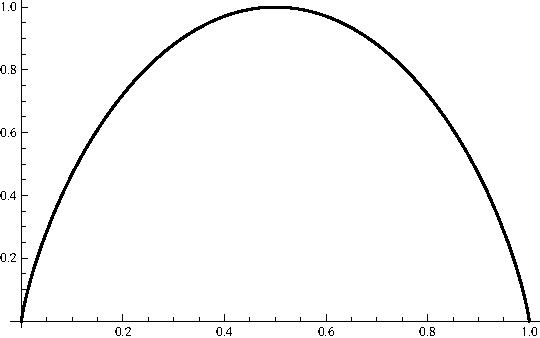
\includegraphics{figures/entropy2.pdf}}
\caption{The entropy function $H(p)$ for a two-value distribution}
\end{center}
\end{figure}

\begin{lem}[Gibbs's inequality]
If $(p_1,\ldots,p_d)$ is a probability vector and $(q_1,\ldots,q_d)$ is a \emph{sub-probability} vector, i.e., we have $p_k,q_k\ge 0$, $\sum_k p_k = 1$ and $\sum q_k \le 1$, then
$$ -\sum_{k=1}^d p_i \log p_i \le -\sum_{k=1}^d p_i \log q_i, $$
with equality holding if and only the two vectors are equal.
\end{lem}

\begin{proof} The form of the inequality is unchanged by changing the logarithm basis, so we use the natural logarithm. Since $\log x \le x-1$ for all $x>0$, we have
\begin{align*}
-\sum_{k=1}^d p_k (\log q_k-\log p_k) &=
-\sum_{k=1}^d p_k \log\left( \frac{q_k}{p_k}\right) 
\ge -\sum_{k=1}^d p_k \left( \frac{q_k}{p_k}-1 \right) \\ &= -\sum_k q_k + \sum_k p_k \ge -1+1 = 0. 
\end{align*}
\end{proof}

\begin{lem}[Properties of the entropy function] 
\label{lem-entropy-properties}
The entropy function of $d$-dimensional probability vectors $(p_1,\ldots,p_d)$ satisfies:
\begin{enumerate}
\item $0 \le H(p_1,\ldots,p_d) \le \log_2 d$
\item $H(p_1,\ldots,p_d)=0$ if and only if $p_k=1$ for some $k$ (and all the other $p_j$'s are 0).
\item $H(p_1,\ldots,p_d)=\log_2 d$ if and only if $p_k=1/d$ for all $k$.
\item $H(\mathbf{p}\otimes \mathbf{q}) = H(\mathbf{p}) + H(\mathbf{q})$, where if $\mathbf{p}=(p_1,\ldots,p_d)$ and $\mathbf{q}=(q_1,\ldots,q_\ell)$, we use the notation $\mathbf{p}\otimes\mathbf{q}$ to denote the probability vector $(p_i q_j)_{i,j}$ on the product of two alphabets of sizes $d$ and $\ell$.
\item $H(p_1,\ldots,p_d)$ is a concave function.
\end{enumerate}
\end{lem}

\begin{exercise}
Prove Lemma~\ref{lem-entropy-properties}.
\end{exercise}

\subsection{The noiseless coding theorem}

Our first interpretation of the entropy function will be in terms of the problem of \textbf{noiseless coding}. Recall that the information source emits symbols in the finite alphabet $A=\{\alpha_1,\ldots,\alpha_d\}$. To transmit the symbol over a digital communication channel or store it on a computer storage system (which is the same as transmission, except we're transmitting it to ourselves in the future rather than to a different physical location), we need to encode the symbols as binary bits. We assume that the storage system or communication system are \textbf{noiseless}, i.e., no corruption of our data is expected to occur.

What is a good way to encode the symbols as binary bits? A naive approach would be to allocate $d$ distinct binary strings, one for each of the symbols. Since the strings need to be distinct so that the transmission can be decoded on the other end, obviously it is necessary (and sufficient) for the strings to be of length $\lceil \log_2 d\rceil$. Thus, in terms of efficiency, this method uses the channel approximately $\log_2 d$ times for every symbol encoded.

But perhaps we can do better? For example, it is possible that some of the symbols occur more frequently than others. A more sophisticated approach would be to assign binary strings of \emph{different} lengths to the different symbols, assigning the shorter strings to more frequently occurring symbols. One must be careful however to make sure that the transmission, which may consist of the concatenation of several of the strings used to encode a succession of source symbols, can be faithfully recovered. This leads to the idea of \textbf{codes}.

\begin{defi} Let $\{0,1\}^*=\cup_{n=1}^\infty \{0,1\}^n$ be the set of all finite binary sequences (which we will call \textbf{words} or \textbf{strings}). A \textbf{code} for the alphabet $A=\{ \alpha_1,\ldots,\alpha_d\}$ is a collection $(w_k)_{k=1}^d$ of words in $\{0,1\}^*$. We say the code is \textbf{uniquely decodable} if any word formed as a concatenation
$w_{j_1}w_{j_2}\ldots w_{j_m}$
of words in the code can be decoded in a unique way, i.e., it is not equal to any other concatenation of words from the same code. We say that the code is a \textbf{prefix code} if no word $w_i$ in the code is a prefix of another word $w_j$. 
\end{defi}

It is obvious that any prefix code is uniquely decodable, since, when reading a concatenation of words, we know immediately when a word terminates and the next word begins. Not all uniquely decodable codes are prefix codes, however (the code $0, 01, 011$ is an example). It is however true that uniquely decodable codes that are not prefix codes are in some sense pointless and for all practical purposes they may be ignored --- see Exercise~\ref{exer-uniquely-decodable} at the end of this section to understand why. Prefix codes, on the other hand, are extremely useful in both theory and applications, and used by people (e.g., punctuation marks in language, the telephone directory), computers (innumerable examples) and even nature (the genetic code encodes amino acids used as building blocks of proteins as triplets of nucleotides in DNA).

For a word $w\in \{0,1\}^*$, denote its length by $\ell(w)$. Given a code $w_1,\ldots,w_d$ associated with an information source that emits a random symbol $\alpha_1,\ldots,\alpha_d$ with respective probabilities $p_1,\ldots,p_d$, denote by $L$ the (random) word length, i.e., $L=\ell(w_k)$ with probability $p_k$ for $k=1,\ldots,d$. A crucial quantity that we are interested in is the \textbf{expected word length}
$$ \expec(L) = \sum_{k=1}^d p_k \ell(w_k). $$
By the law of large numbers, this quantity says how many bits we will need to transmit over the channel for every source symbol coded when encoding very long strings of source symbols. How small can we make $L$? The following famous result answers this fundamental question.

\begin{thm}[Noiseless coding theorem] Let $(p_1,\ldots,p_d)$ be a probability vector. Then:
\begin{enumerate}
\item If $(w_1,\ldots,w_d) \in \{0,1\}^* $ is a prefix code for the source, then the expected word length satisfies
$$ \expec(L) = \sum_{k=1}^d p_k \ell(w_k) \ge H(p_1,\ldots, p_d). $$
\item A prefix code $(w_1,\ldots,w_d) \in \{0,1\}^* $ may be found for which the expected word length satisfies
$$ \expec(L) = \sum_{k=1}^d p_k \ell(w_k) \le H(p_1,\ldots, p_d) + 1. $$
\end{enumerate}
\end{thm}

To prove the theorem, we need an auxiliary result:

\begin{thm}[Kraft's inequality] \ \\ \vspace{-20.0pt}
\begin{enumerate}
\item If $w_1,\ldots,w_d$ is a prefix code then $\sum_{k=1}^d 2^{-\ell(w_k)} \le 1$. 
\item Conversely, if $\ell_1,\ldots,\ell_d$ are positive integers satisfying $\sum_{k=1}^d 2^{-\ell_k} \le 1$, then there exists a prefix code $w_1,\ldots,w_k$ with $\ell(w_k)=\ell_k$.
\end{enumerate}
\end{thm}

\begin{proof}
For the first claim, for each word $w_k=a_1\ldots a_{\ell(w_k)}$ define a real number $x_k$ by
$$ x_k = \sum_{j=1}^{\ell(w_k)} a_j 2^{-j} = (0.a_1a_2\ldots a_{\ell(w_k)})_{\textrm{binary}}, $$
and consider the interval $I_k = (x_k,x_k+2^{-\ell(w_k)})$ (a sub-interval of $(0,1)$). The fact that the code is a prefix code is equivalent to the statement that the intervals $I_k$, $k=1,\ldots,d$ are disjoint. It follows that $\sum_k |I_k| = \sum_k 2^{-\ell(w_k)} \le 1$.

For the other direction, starting with the lengths $\ell_1,\ldots,\ell_d$, first assume without loss of generality that $\ell_1\le \ell_2\le \ldots \le \ell_k$ (if not, relabel the indices). It is clear that we can inductively construct disjoint dyadic intervals $I_1,\ldots,I_k \subset (0,1)$ such that each $I_k$ is of the form $(x_k,x_k+2^{-\ell_k})$ where $x_k$ has a binary expansion of length $\ell_k$ (take $x_1=0$ and let each $x_k$ for $k\ge 2$ be the rightmost endpoint of $I_{k-1}$; the construction will work because of the assumption that $\sum_{k=1}^d 2^{-\ell_k} \le 1$, so the intervals never leave $(0,1)$, and the assumption that the lengths are increasing, which implies that the length of the binary expansion of $x_k$ is at most $\ell_{k-1}$). The code words $w_1,\ldots,w_k$ are then taken as the respective binary expansions of $x_1,\ldots,x_d$, where for each $x_k$, if the binary expansion is shorter than $\ell_k$ (as in the case of $x_1=0$), it is brought to the right length by padding it with zeros.
\end{proof}

\begin{proof}[Proof of the noiseless coding theorem]
For the first part of the theorem, observe that since $\sum_{k=1}^d 2^{-\ell(w_k)}\le 1$ by Kraft's inequality, we can apply Gibbs's inequality to the two vectors $(p_1,\ldots,p_k)$ and $(2^{-\ell(w_1)}, \ldots, 2^{-\ell(w_d)})$, to get that
$$
\expec(L) = \sum_{k=1}^d p_k \ell(w_k) = -\sum_{k=1}^d p_k \log_2 \left(2^{-\ell(w_k)}\right) \ge -\sum_{k=1}^d p_k \log_2 p_k = H(p_1,\ldots,p_d).
$$
For the second part, for each $1\le k\le d$ let $\ell_k = \lceil -\log_2 p_k\rceil$, so that the inequality
$ 2^{-\ell_k} \le p_k < 2^{-\ell_k+1} $ holds. Then $\sum_k 2^{-\ell_k} \le \sum_k p_k = 1$, so by Kraft's inequality we can find a prefix code $w_1,\ldots,w_k$ with word lengths $\ell_1,\ldots,\ell_k$. For this code, we have
$$
\expec(L) = \sum_{k=1}^d p_k \ell_k = -\sum_{k=1}^d p_k \log_2\left(2^{-\ell_k}\right)
\le -\sum_{k=1}^d p_k \log_2 (p_k/2) = H(p_1,\ldots,p_d) + 1.
$$
\end{proof}

While the noiseless coding theorem clearly indicates that the entropy $H=H(p_1,\ldots,p_d)$ is an interesting number, one might argue that the true minimal expected coding word length, which (by the theorem) lies somewhere in the interval $[H,H+1]$ (but which in practice may be hard to compute), is a more meaningful measure of the information content of a random symbol sampled from the distribution $p_1,\ldots,p_d$. For example, for a binary source information source with distribution $(p,1-p)$ the ``optimal expected word length'' is exactly $1$ bit per source symbol. However, in an asymptotic sense the entropy really is the more meaningful number; the trick is to cluster the source symbols into groups of fixed length and encode these longer strings, as the following reformulated version of the noiseless coding theorem explains.

\begin{cor}[Noiseless coding theorem, version 2]
Let $\mathbf{p}=(p_1,\ldots,p_d)$ be a probability vector. Then:
\begin{enumerate}
\item Any prefix code for a source with distribution $\mathbf{p}$ has expected word length $\ge H(\mathbf{p})$.
\item For any $\epsilon>0$, we can find an integer $N$ large enough and a prefix code for a source with distribution $\mathbf{p}^{\otimes N}=\mathbf{p}\otimes\ldots\otimes\mathbf{p}$ (the distribution of a vector of $N$ independent samples from $\mathbf{p}$) which has expected word length $\le N(H(\mathbf{p})+\epsilon)$; that is, the expected word length \emph{per symbol coded} is at most $H(\mathbf{p})+\epsilon$.
\end{enumerate}
\end{cor}

\begin{proof} For part 2, take $N=1/\epsilon$ and apply the first version of the noiseless coding theorem to the distribution $\mathbf{p}^{\otimes N}$, making use of property~4 in Lemma~\ref{lem-entropy-properties}.
\end{proof}

To summarize, this last formulation of the noiseless coding theorem gives a meaning to the entropy function as measuring precisely the difficulty of (noiselessly) coding the source, in an asymptotic sense: first, any code will require sending at least $H(p)$ binary bits over the communication channel; conversely, one can approach this lower bound asymptotically by coding for multiple symbols simultaneously.

\begin{exercise}
\label{exer-uniquely-decodable}
Prove that any uniquely decodable code can be replaced by a prefix code with the same word lengths.
\end{exercise}


\subsection{The asymptotic equipartition property}

A related way of thinking about entropy is in terms of data compression: given a string of source symbols of length $n$ (which could itself be a binary string in the case of a $2$-symbol alphabet), how much can we compress it, i.e., what is the typical length of a binary string we'll need to represent it? The noiseless coding theorem says that on the average we'll need around $n H(p_1,\ldots,p_d)$ bits; however, the theorem doesn't address the question of how many bits we'll need \emph{typically} (that is, with probability close to $1$)? Of course, these questions are in general not equivalent: for example, it may seem conceivable that the reason the average number of bits is around $nH(p_1,\ldots,p_d)$ is that around half the time we need a much smaller number of bits, and the other half of the time we need approximately twice as many. The following result, known as the \textbf{asymptotic equipartition property}, demonstrates that in fact in this case the typical behavior is the same as the average one.

\begin{thm}[Asymptotic equipartition property for an i.i.d.\ source]
Let $X_1,X_2,\ldots$ be an i.i.d.\ information source over the alphabet $A=\{\alpha_1,\ldots,\alpha_d\}$, distributed according to the probability vector $\mathbf{p}=(p_1,\ldots,p_d)$ as before. Fix $\epsilon>0$. There exists a large enough integer $N$ such that the sequences $A^N$ can be partitioned into a disjoint union of sequences of two types, namely,
$$ A^N = T \sqcup E, $$
where the sequences in $T$ and $E$ are called the \textbf{typical} and \textbf{exceptional} sequences, respectively, such that the following properties hold:
\begin{enumerate}
\item $\prob((X_1,\ldots,X_N) \in E) < \epsilon,$ (i.e., the exceptional sequences are indeed exceptional).
\item The probability of observing each typical sequence $(x_1,\ldots,x_N)\in T$ satisfies
\begin{equation} \label{eq:aep-prob-bound}
2^{-N\left(H(\mathbf{p}) + \epsilon\right)} \le 
\prob((X_1,\ldots,X_N)=(x_1,\ldots,x_N)) \le 
2^{-N\left(H(\mathbf{p}) - \epsilon\right)}.
\end{equation}
\item Consequently, assuming $\epsilon<1/2$, the number of typical sequences satisfies
\begin{equation} \label{eq:aep-numtypical}
2^{N (H(\mathbf{p})-\epsilon)+1} \le |T| \le 2^{N (H(\mathbf{p})+\epsilon)}.
\end{equation}
\end{enumerate}
\end{thm}

\begin{proof} Define a sequence $Z_1, Z_2, \ldots $ of i.i.d.\ random variables by
$$ Z_n = -\sum_{k=1}^d -\log_2 p_k \ind_{\{X_n = \alpha_k\}}, $$
and denote $S_n = \sum_{j=1}^n Z_j$. By the weak law of large numbers we have that
$$ \frac{1}{n} S_n \xrightarrow[n\to\infty]{\textrm{P}} \expec(Z_1) = H(\mathbf{p}), $$
and therefore for large enough $N$, we have
\begin{equation} \label{eq:aep-typicalevent}
\prob\left(\left|\frac{1}{N}S_N- H(\mathbf{p})\right|\le \epsilon \right)\ge 1-\epsilon.
\end{equation}
Call the event on the left-hand side $B$. This is an event that depends on the r.v.'s $X_1,\ldots,X_N$, so it can be represented as a disjoint union of events of the form
$$ B = \bigsqcup_{(x_1,\ldots,x_n)\in T} \{ (X_1,\ldots,X_N) = (x_1,\ldots,x_n) \} $$
for some set $T\subset A^N$ of sequences. This will be our set of typical sequences; the exceptional sequences are defined as the complementary set $E = A^N\setminus T$.

We now claim that $T$ and $E$ satisfy the properties in the theorem. Property~1 holds automatically by \eqref{eq:aep-typicalevent}. For property~2, observe that if $(x_1,\ldots,x_N)=(\alpha_{j_1},\ldots,\alpha_{j_N})\in T$ then by the definition of the event $B$ we have
$$
N\left(H(\mathbf{p}) - \epsilon\right) \le 
-\sum_{n=1}^N \log_2 p_{j_n} \le N\left(H(\mathbf{p}) + \epsilon\right),
$$
or equivalently
$$
2^{-N\left(H(\mathbf{p}) + \epsilon\right)} \le 
\prod_{n=1}^N p_{j_n} \le 
2^{-N\left(H(\mathbf{p}) - \epsilon\right)}.
$$
But $\prod_{n=1}^N p_{j_n}$ is exactly $\prob((X_1,\ldots,X_N)=(x_1,\ldots,x_N))$, so we get \eqref{eq:aep-prob-bound}.
On the other hand, the total probability of observing \emph{any} typical sequence is $\prob(B)$, which is bounded between $1-\epsilon$ and $1$ (hence, between $1/2$ and $1$, if we assume $\epsilon<1/2$). This implies \eqref{eq:aep-numtypical}.
\end{proof}

The implication of the theorem is that since the number of typical sequences is around $2^{n(H(\mathbf{p})\pm \epsilon)}$, we can encode them using a binary string of length $\approx nH(\mathbf{p})$. How easy this is to do in practice is a different question (some very practical techniques exist that are not difficult to implement --- for example, two well-known methods are known as Huffman coding and Lempel-Ziv coding).

\begin{exercise} Use the asymptotic equipartition property to give an alternate proof of the reformulated version of the noiseless coding theorem.
\end{exercise}

\subsection{Ergodic sources and the Shannon-McMillan-Breiman theorem}

We are now ready to discuss the situation for a general stationary ergodic source $X_1,X_2,\ldots$. It turns out that a version of the asymptotic equipartition property is valid for such a source. To prove it, we first need to correctly define the entropy of the source, and to prove an important convergence result that replaces the (trivial) use of the law of large numbers in the case of an i.i.d.\ source.

For a sequence $(x_1,\ldots,x_n)\in A^n$, denote 
\begin{align}
p(x_1,\ldots,x_n) &= \prob((X_1,\ldots,X_n)=(x_1,\ldots,x_n)), \label{eq:psymbols1} \\
p(x_n\,|\,x_1,\ldots,x_{n-1}) &= \prob(X_n=x_n\,|\,(X_1,\ldots,X_{n-1})=(x_1,\ldots,x_{n-1})), 
\label{eq:psymbols2} \\
H_n &= -\expec(\log_2 p(X_n\,|\,X_1,\ldots,X_{n-1})).
\label{eq:psymbols3}
\end{align}
In information theory the quantity $H_n$ is often denoted by $H(X_n\,|\, X_1,\ldots,X_{n-1})$; it is a special case of a \textbf{conditional entropy}.

\begin{lem} \label{lem-entropy-ergodic}
$(H_n)_{n=1}^\infty$ is a weakly monotone decreasing sequence, hence converges to a limit
\begin{equation} \label{eq:entropy-ergodic} 
H \equiv \lim_{n\to\infty} H_n \ge 0.
\end{equation}
\end{lem}

The proof follows by induction by applying the result of the following exercise.

\begin{exercise} Let $A=\{\alpha_1,\ldots,\alpha_d \}$ and $B=\{\beta_1,\ldots,\beta_m \}$ be two finite sets. If $X,Y$ are two random variables such that $\prob(X\in A, Y\in B)=1$, the conditional entropy $H(X\,|\,Y)$ is defined by
\begin{align*}
H(X\,|\,Y) &= -\sum_{j=1}^m \sum_{k=1}^d \prob(X=\alpha_k, Y=\beta_j) \log_2 \prob(X = \alpha_k\,|\,Y=\beta_j)
\\ &= \sum_{j=1}^m \prob(Y=\beta_j) H(X\,|\,Y=\beta_j).
\end{align*}
I.e., $H(X\,|\,Y)$ is the average of the entropies of the conditional distributions of $X$ given the outcome of $Y$. Prove that $H(X\,|\,Y) \le H(X)$, with equality if and only if $X$ and $Y$ are independent. Deduce also that $H(X\,|\,Y,Z) \le H(X\,|\,Z)$ if $Z$ is another random variable, and explain why this implies Lemma~\ref{lem-entropy-ergodic}.
\end{exercise}



We refer to $H$ in \eqref{eq:entropy-ergodic} as \textbf{the entropy of the source $(X_n)_{n=1}^\infty$}. There is an equivalent way to define it which is also interesting. Since $H_n\to H$, the Ces\`aro averages of $(H_n)_n$ also converge to $H$, i.e.,
$$ \frac{1}{n}(H_1+\ldots+H_n) \to H \textrm{ as }n\to\infty. $$
The average on the left-hand side can be written as
\begin{align*}
-\frac1n \expec&\Big[ \log_2 p(X_1) + \log_2 p(X_2\,|\,X_1)
+ \log_2 p(X_3\,|\,X_1,X_2) + \ldots + p(X_n\,|\,X_1,\ldots,X_{n-1}) \Big]
\\ &= -\frac1n \expec \left[\log_2 p(X_1,\ldots,X_n)\right] = \frac{1}{n}H(X_1,\ldots,X_n).
\end{align*}
(Here, $H(X_1,\ldots,X_n)$ refers to the entropy of the discrete vector random variable $(X_1,\ldots,X_n)$, which takes values in the finite set $A^n$.) Thus, $H$ may be interpreted as the limit of $\frac{1}{n} H(X_1,\ldots,X_n)$, i.e., the asymptotic entropy per symbol in a long string of symbols sampled from the source.

The importance of $H$ is explained by the following fundamental result, sometimes referred to as ``the individual ergodic theorem of information theory''.

\begin{thm}[Shannon-McMillan-Breiman theorem]
\label{thm-shannon-mcmillan-breiman}
We have the almost sure convergence
\begin{equation} \label{eq:shannon-mcmillan-breiman}
-\frac{1}{n}\log_2(p(X_1,\ldots,X_n)) \xrightarrow[n\to\infty]{\textrm{a.s.}} H
\end{equation}
\end{thm}

\begin{lem} 
\label{lem-aep-lemma}
If $(Z_n)_n$ is a sequence of nonnegative random variables such that $\expec(Z_n)\le 1$ for all $n$, then
\begin{equation} \label{eq:aep-lemma}
\prob\left(\limsup_{n\to\infty} \frac{1}{n} \log Z_n \le 0\right) = 1.
\end{equation}
\end{lem}

\begin{proof}
Fix $\epsilon>0$. By Markov's inequality, we have
$$ \prob(n^{-1} \log Z_n \ge \epsilon) = \prob(Z_n \ge e^{n\epsilon}) \le e^{-n\epsilon}. $$
Since $\sum_n e^{-n\epsilon}<\infty$, the first Borel-Cantelli implies that 
$\prob(n^{-1} \log Z_n \ge \epsilon \ \textrm{i.o.}) = 0$. This is true for any $\epsilon>0$, so taking a union of these events over $\epsilon=1/k, k=1,2,\ldots$ gives \eqref{eq:aep-lemma}.
\end{proof}

\begin{proof}[Proof of Theorem~\ref{thm-shannon-mcmillan-breiman}] As explained in Section~\ref{sec-stationary}, we may assume without loss of generality that the sequence $(X_n)_n$ is actually a two-sided ergodic stationary sequence $(X_n)_{n=-\infty}^\infty$. We start by giving yet another, more subtle, interpretation of the source entropy $H$. By stationarity, we may rewrite $H_n$ as
$$ H_n = -\expec(\log_2 p(X_0\,|\,X_{-n+1},\ldots,X_{-1})) = -\sum_{j=1}^d \expec\Big[ L\big(
\condexp{\ind_{\{X_0=\alpha_j\}}}{\mathcal{G}_{-n+1}^{-1}} \big)\Big], 
$$
where we denote $L(p) = p\log_2 p$ and $\mathcal{G}_s^t = \sigma(X_m\,;\, s\le m\le t)$. Note that for each $j$, the expression $\condexp{\ind_{\{X_0=\alpha_j\}}}{\mathcal{G}_{-n+1}^{-1}} \big)$ inside the conditional expectation above forms a martingale (as a function of $n$) taking values in $[0,1]$. By L\'evy's martingale convergence theorem (Theorem~\ref{eq:levy-martingale-conv}), we have
$$ \condexp{\ind_{\{X_0=\alpha_j\}}}{\mathcal{G}_{-n+1}^{-1}} \big) \to \condexp{\ind_{\{X_0=\alpha_j\}}}{\mathcal{G}_{-\infty}^{-1}} \ \textrm{ a.s. as }n\to\infty.
$$
Since $L(\cdot)$ is a bounded continuous function on $[0,1]$, using the bounded convergence theorem we therefore get also that 
\begin{align*} H_n 
&\xrightarrow[n\to\infty]{} \expec\left[ -\sum_{j=1}^d \condexp{\ind_{\{X_0=\alpha_j\}}}{\mathcal{G}_{-\infty}^{-1}}
\log_2 \condexp{\ind_{\{X_0=\alpha_j\}}}{\mathcal{G}_{-\infty}^{-1}}
\right] 
\end{align*}
Of course, the limit of $H_n$ is $H$, so we have derived another formula
\begin{equation} \label{eq:entropy-newformula}
H = \expec\left[ -\sum_{j=1}^d \condexp{\ind_{\{X_0=\alpha_j\}}}{\mathcal{G}_{-\infty}^{-1}}
\log_2 \condexp{\ind_{\{X_0=\alpha_j\}}}{\mathcal{G}_{-\infty}^{-1}}
\right] 
\end{equation}
for the source entropy. Furthermore, this expression can be rewritten in the simpler form
\begin{equation} \label{eq:entropy-simpler}
H = -\expec \log_2 p(X_0\,|\,\mathcal{G}_{-\infty}^{-1}),
\end{equation}
where we adopt the notation (in the same vein as \eqref{eq:psymbols1} and \eqref{eq:psymbols2})
\begin{equation} \label{eq:psymbols-generalized}
p(x\,|\,\mathcal{G}_s^t) = \condprob{X_{t+1}=x}{\mathcal{G}_s^t}.
\end{equation}
To see why, note that
$$ p(X_0\,|\,\mathcal{G}_{-\infty}^{-1}) = \sum_{j=1}^d \ind_{\{X_0=\alpha_j\}} p(\alpha_j\,|\,\mathcal{G}_{-\infty}^{-1}), $$
and use this to write the right-hand side of \eqref{eq:entropy-simpler} as
\begin{align*}
-\expec \log_2 p(X_0\,|\,\mathcal{G}_{-\infty}^{-1})
&=
-\sum_{j=1}^d \expec\Big[
\condexp{ 
\ind_{\{X_0=\alpha_j\}}
\log_2 p(\alpha_j\,|\,\mathcal{G}_{-\infty}^{-1})
}{\mathcal{G}_{-\infty}^{-1}}
\Big]
\\ &= -\sum_{j=1}^d \expec\Big[ \log_2 p(\alpha_j\,|\,\mathcal{G}_{-\infty}^{-1})
\condexp{\ind_{\{X_0=\alpha_j\}}}{\mathcal{G}_{-\infty}^{-1}}
\Big]
\\ &= -\sum_{j=1}^d \expec\Big[
p(\alpha_j\,|\,\mathcal{G}_{-\infty}^{-1})
\log_2 p(\alpha_j\,|\,\mathcal{G}_{-\infty}^{-1})
\Big],
\end{align*}
which is the same as the right-hand side of \eqref{eq:entropy-newformula}.

Having derived the representation~\eqref{eq:entropy-simpler} for the source entropy, we now apply another piece of heavy machinery, the ergodic theorem, which implies that
$$ -\frac{1}{n} \sum_{k=0}^{n-1} \log_2 p(X_k\,|\,\mathcal{G}_{-\infty}^{k-1}) \xrightarrow[n\to\infty]{\textrm{a.s.}} H. $$
Furthermore, one may verify without much difficulty that this ergodic average can be rewritten in the form
\begin{equation} \label{eq:aep-ergodic-average1}
 -\frac{1}{n} \sum_{k=0}^{n-1} \log_2 p(X_k\,|\,\mathcal{G}_{-\infty}^{k-1}) = -\frac{1}{n} \log_2 p(X_0,\ldots,X_{n-1}\,|\,\mathcal{G}_{-\infty}^{-1}).
\end{equation}
(where the notation $p(x_0,\ldots,x_{n-1}\,|\,\mathcal{G}_s^t)$ is defined as an obvious generalization of \eqref{eq:psymbols-generalized}). So we conclude that 
$$ -\frac{1}{n} \log_2 p(X_0,\ldots,X_{n-1}\,|\,\mathcal{G}_{-\infty}^{-1})
\to H \ \textrm{ a.s. as }n\to\infty. $$
This fact bears some resemblance to the claim \eqref{eq:shannon-mcmillan-breiman} that we are trying to prove, and indeed, we can deduce ``half'' of our result from it --- a one-sided asymptotic bound --- using Lemma~\ref{lem-aep-lemma}, as follows. Define a sequence of random variables $(Z_n)_{n=1}^\infty$ by $Z_n = \frac{p(X_0,\ldots,X_{n-1})}{p(X_0,\ldots,X_{n-1}\,|\,\mathcal{G}_{-\infty}^{-1})}$. We have
\begin{align}
\expec(Z_n) &= \expec \left[\condexp{Z_n}{\mathcal{G}_{-\infty}^{-1}}\right]
\nonumber \\ &= \expec\left[
\sum_{x_0,\ldots,x_{n-1}\in A} 
\condexp{
\frac{p(x_0,\ldots,x_{n-1})}{p(x_0,\ldots,x_{n-1}\,|\,\mathcal{G}_{-\infty}^{-1})}
p(x_0,\ldots,x_{n-1}\,|\,\mathcal{G}_{-\infty}^{-1})
}{\mathcal{G}_{-\infty}^{-1}}
\right]
\nonumber \\ &= \sum_{x_0,\ldots,x_{n-1}\in A} p(x_0,\ldots,x_{n-1}) = 1.
\label{eq:aep-expec1}
\end{align}
So, we are in the situation described in Lemma~\ref{lem-aep-lemma}, and we conclude that almost surely we have the inequality
\begin{align*}
0 &\le -\limsup_{n\to\infty} \frac{1}{n} \log_2 Z_n = \liminf_{n\to\infty} \left(-\frac{1}{n} \log_2 Z_n\right)
 \\ &= \liminf_{n\to\infty} \left[
-\frac{1}{n} \log_2 p(X_0,\ldots,X_{n-1}) + \frac{1}{n}\log_2 p(X_0,\ldots,X_{n-1}\,|\,\mathcal{G}_{-\infty}^{-1}) \right]
\\ &=
\liminf_{n\to\infty} \left[-\frac{1}{n} \log_2 p(X_0,\ldots,X_{n-1})\right] + 
\lim_{n\to\infty}
\frac{1}{n}\log_2 p(X_0,\ldots,X_{n-1}\,|\,\mathcal{G}_{-\infty}^{-1})
\\ &= 
\liminf_{n\to\infty} \left[-\frac{1}{n} \log_2 p(X_0,\ldots,X_{n-1})\right] - H.
\end{align*}
That is, we have proved that the inequality
\begin{equation} \label{eq:smb-first-half}
\liminf_{n\to\infty} \left[-\frac{1}{n} \log_2 p(X_0,\ldots,X_{n-1})\right] \ge H.
\end{equation}
holds with probability $1$.

To finish the proof, we will now prove an asymptotically matching upper bound; more precisely, we claim that for each fixed $k\ge1$, almost surely the inequality
\begin{equation} \label{eq:smb-second-half}
-\limsup_{n\to\infty} \frac{1}{n} \log_2 p(X_0,\ldots,X_{n-1}) \le H_k
\end{equation}
holds. Since $H_k \searrow H$, the inequalities \eqref{eq:smb-first-half} and \eqref{eq:smb-second-half} together imply \eqref{eq:shannon-mcmillan-breiman}.
To this end, for each $k\ge 1$ we define the ``$k$th order Markov approximation'' to the function $p(x_1\ldots,x_n)$ by
\begin{align*}
 p_k(x_1,\ldots,x_n) &= p(x_1,\ldots,x_k) p(x_{k+1}\,|\,x_1,\ldots,x_k)
p(x_{k+2}\,|\,x_2,\ldots,x_{k+1}) \cdots p(x_n\,|\, x_{n-k},\ldots, x_{n-1}) \\ &= p(x_1,\ldots,x_k)
\prod_{j=k+1}^n p(x_j\,|\, x_{j-k},\ldots,x_{j-1}) \qquad \ \ \ (n\ge k).
\end{align*}
The idea in this definition is that $p_k(x_1,\ldots,x_k)$ is the symbol distribution of a modified source process $(X_n^{(k)})_{n=1}^\infty$ in which the conditional distribution of observing a symbol $x_n$ given the past symbols $x_1,\ldots,x_{n-1}$ is computed from the symbol distribution of the original process by ``forgetting'' all the symbols before $x_{n-k}$, i.e., using only the information in the past $k$ symbols. This modified source is a generalized type of Markov chain known as a \textbf{Markov chain of order $k$} or \textbf{Markov chain with memory $k$}.

Now observe that we have an expansion analogous to \eqref{eq:aep-ergodic-average1}, namely
$$
-\frac{1}{n} \log_2 p_k(X_0,\ldots,X_{n-1}) = -\frac{1}{n} \log_2 p(X_0,\ldots,X_{k-1}) - \frac{1}{n} \sum_{j=k}^{n-1} \log_2 p(X_j\,|\,X_{j-k},\ldots,X_{j-1}).
$$
Combining it with an application of the ergodic theorem, we deduce that
$$
-\frac{1}{n} \log_2 p_k(X_0,\ldots,X_{n-1}) \xrightarrow[n\to\infty]{\textrm{a.s.}} -\expec \big(\log_2 p(X_k\,|\,X_0,\ldots,X_{k-1})\big) = H_k.
$$
This again bears a resemblance to \eqref{eq:shannon-mcmillan-breiman}, and we can relate the two using the lemma. Define a sequence $(Y_n)_{n=k}^\infty$ of random variables by $Y_n = \frac{p_k(X_0,\ldots,X_{n-1})}{p(X_0,\ldots,X_{n-1})}$. A short computation similar to \eqref{eq:aep-expec1}, which we leave to the reader to verify, shows that $\expec(Y_n) \le 1$ for all $n\ge k$, so from Lemma~\ref{lem-aep-lemma} we get that almost surely,
\begin{align*}
0 &\ge \limsup_{n\to\infty} \frac{1}{n} \log_2 Y_n 
 \\ &= \limsup_{n\to\infty} \left[
\frac{1}{n} \log_2 p_k(X_0,\ldots,X_{n-1}) - \frac{1}{n}\log_2 p(X_0,\ldots,X_{n-1}) \right]
\\ &=
-H_k + \limsup_{n\to\infty} \left(- \frac{1}{n}\log_2 p(X_0,\ldots,X_{n-1}) \right),
\end{align*}
which proves \eqref{eq:smb-second-half} and thus finishes the proof.
\end{proof}


\begin{thm}[Asymptotic equipartition property for an ergodic source]
Let $X_1,X_2,\ldots$ be a stationary ergodic information source over the alphabet $A=\{\alpha_1,\ldots,\alpha_d\}$. Fix $\epsilon>0$. There exists a large enough integer $N$ such that the sequences $A^N$ can be partitioned into a disjoint union of typical and exceptional sequences, namely, $A^N = T \sqcup E$, such that we have:
\begin{enumerate}
\item $\prob((X_1,\ldots,X_N) \in E) < \epsilon$.
\item $2^{-N\left(H + \epsilon\right)} \le 
\prob((X_1,\ldots,X_N)=(x_1,\ldots,x_N)) \le 
2^{-N\left(H - \epsilon\right)}$ for each typical sequence $(x_1,\ldots,x_N)\in T$.
\item Consequently, assuming $\epsilon<1/2$, the number of typical sequences satisfies
$$
2^{N (H-\epsilon)+1} \le |T| \le 2^{N (H+\epsilon)}.
$$
\end{enumerate}
\end{thm}

\begin{proof} The proof is completely analogous to the proof of the i.i.d.\ case from the previous section; the random variable $S_n$ is redefined as $-\log p(X_1,\ldots,X_n)$, and the use of the weak law of large numbers is replaced by the Shannon-McMillan-Breiman theorem.
\end{proof}

We conclude this chapter with some examples of stationary ergodic sequences and their entropies.

\begin{enumerate}[1.]
\item \textbf{i.i.d.\ source.} If $X_1,X_2,\ldots$ is an i.i.d.\ source whose distribution is described by the probability vector $(p_1,\ldots,p_d)$ then $H_n=H(X_n\,|\,X_1,\ldots,X_{n-1})=H(p_1,\ldots,p_d)$, so the entropy is the usual entropy we discussed before. For example, if $X$ is a Bernoulli random variable satisfying $\prob(X=1)=1/3=1-\prob(X=0)$ then $H=-\tfrac13 \log_2 \tfrac13 - \tfrac23 \log_2 \tfrac23 = 0.91829\ldots $ bits.
\item \textbf{Markov source.} If $X_1,X_2,\ldots$ is a stationary Markov chain, then 
the ``$n$-step'' conditional entropy $H_n$ is given by $H_n=H(X_n\,|\,X_1,\ldots,X_{n-1})= H(X_n\,|\,X_{n-1}) = H(X_2\,|\,X_1)$ by the Markov property, so it is enough to compute this ``$1$-step'' conditional entropy. It is easy to see that this is simply an average with respect to the stationary probabilities of the entropies of each of the rows of the transition matrix.
For example, if the Markov chain has the transition matrix $ \left( \begin{array}{cc} \tfrac12 & \tfrac12 \\ 1&0 \end{array} \right),$
then it is easy to check that $(\tfrac23,\tfrac13)$ is a stationary probability vector for the chain. The entropy is therefore given by
$$ 
H = H(X_2\,|\,X_1) = \tfrac23 H(\tfrac12,\tfrac12) + \tfrac13 H(1,0) = \tfrac23 \cdot 1 = \tfrac 23 = 0.6666\ldots \textrm{ bits}.
$$
Note that this stationary Markov chain has the same one-dimensional marginals as the i.i.d.\ source discussed above. Nonetheless, the entropy is lower, since it measures the incremental amount of information gained by examining a symbol once all the previous symbols are known, which is lower in the case where there is dependence.

\item \textbf{Continued fractions.} From the results discussed in the previous chapter, the entropy of the sequence of quotients $(N\circ G^k)_{k=0}^\infty$ in the continued fraction expansion of a number chosen according to Gauss measure $\gamma$ is equal to $\pi^2/6\log 2$, \emph{when measured in the natural base}. If we want to adhere to the information theory convention and measure this entropy in bits, we must divide by a further factor of $\log 2$, giving an entropy of
$$ \frac{\pi^2}{6(\log 2)^2} = 3.423714\ldots \textrm{ bits}. $$
One way of interpreting this fact is that, as we examine more and more of the continued fraction quotients of a number $x$ chosen uniformly at random from $(0,1)$, on the average each additional quotients will increase our knowledge of the \emph{binary} expansion of $x$ by about $3.42$ additional digits. Incidentally, while preparing these notes I discovered the curious fact (which I have not seen mentioned anywhere) that if we measure the entropy in base~$10$, we get
$$ \frac{\pi^2}{6\log(2)\log(10)} = 1.03064\ldots, $$
i.e., on the average each continued fraction quotient adds an amount of information almost precisely equal to one decimal expansion digit.
\item \textbf{Rotations of the circle.} Let $\alpha\in(0,1)$ be irrational, let $X$ be a random variable taking finitely many values on $((0,1), \mathcal{B}, \textrm{Leb})$, and let $X_n = X\circ R_\alpha^{n-1}$. Then $(X_n)_{n=1}^\infty$ is a stationary ergodic sequence.
\begin{exercise}
Prove that the entropy of this sequence is $0$.
\end{exercise}
\end{enumerate}



%\newpage

\bigskip \bigskip 
\begin{center}
\textbf{End of Part II}
\end{center}

% ***
\end{document}
% ***

\newpage
\begin{center}
\LARGE
Part III --- Markov Chains
\end{center}

\lecturesamepage{Basic theory of Markov chains}

\subsection{Finite state Markov chains}

\subsection{The Frobenius-Perron theorem}

\lecture{Simulating stationary Markov chains}



\end{document}
